\documentclass[UTF8]{ctexart}
\usepackage{lmodern}
\usepackage{amsmath}
\usepackage{graphicx}
\usepackage{float}%提供float浮动环境
\usepackage{booktabs}%提供命令\toprule、\midrule、\bottomrule
\usepackage{geometry}
\usepackage{subfigure}

% \begin{figure}[htbp]
%     \centering
%     \includegraphics[width=0.60\textwidth]{}
% \end{figure}

% \begin{table}[H]
%     \centering
%     \caption{\label{表}\textbf{}}
%     \begin{tabular}{ccc}
%     \toprule

%     \midrule
          
%     \bottomrule
%     \end{tabular}
% \end{table}

% \begin{figure}[htbp]
%     \centering
%       \subfigure{
%       \begin{minipage}[t]{0.50\linewidth}
%       \centering
%       \includegraphics[width=3in]{D-eta-k.png}
%       \end{minipage}%
%     }%
%       \subfigure{
%       \begin{minipage}[t]{0.50\linewidth}
%       \centering
%       \includegraphics[width=3in]{D-eta-k^2.png}
%       \caption{fig2}
%       \end{minipage}%
%     }%
  
%   \end{figure}

\geometry{a4paper,left=2cm,right=2cm,top=2cm,bottom=2cm}

\title{{电子技术基础实验} \\ \textbf{实验三\ 三极管放大电路2}}
\author{\\\textbf{祝尔乐}
        \\\textbf{未央-电01}
        }
\date{\textbf{\today}}

\begin{document}
\maketitle

\section*{一.实验目的}
\subsubsection*{
1、了解振荡器工作原理。}
\subsubsection*{
2、了解电子电路中的混沌现象。}
\subsubsection*{
3、熟悉电路仿真与调试。}



\section*{二.实验内容}

\subsection*{1.混沌电路}

\begin{figure}[htbp]
    \centering
    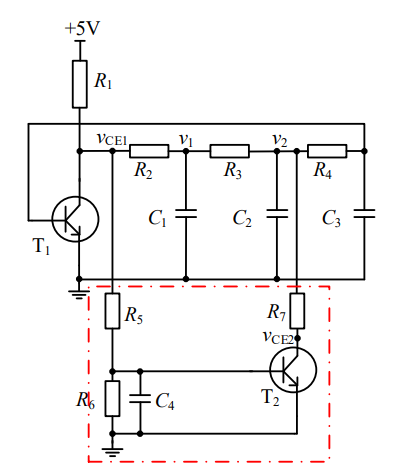
\includegraphics[width=0.40\textwidth]{1-电路图.png}
    \caption{电路图}
\end{figure}
电路参数:R1,R2: $5k \Omega$;R3,R4: $10k \Omega$;R5: $31k \Omega$(
用 50$k \Omega$ 可调);R6: 47$k \Omega$;R7: 15$k \Omega$;
C1-C3: 1nF;C4:360pF;
T1,T2:BC547B

\subsubsection*{(1)不接入图中虚线框内的电路,测量电路中各点电压波形图,并与理论
及仿真结果比较。}

先对电路进行仿真:
\begin{figure}[htbp]
  \centering
  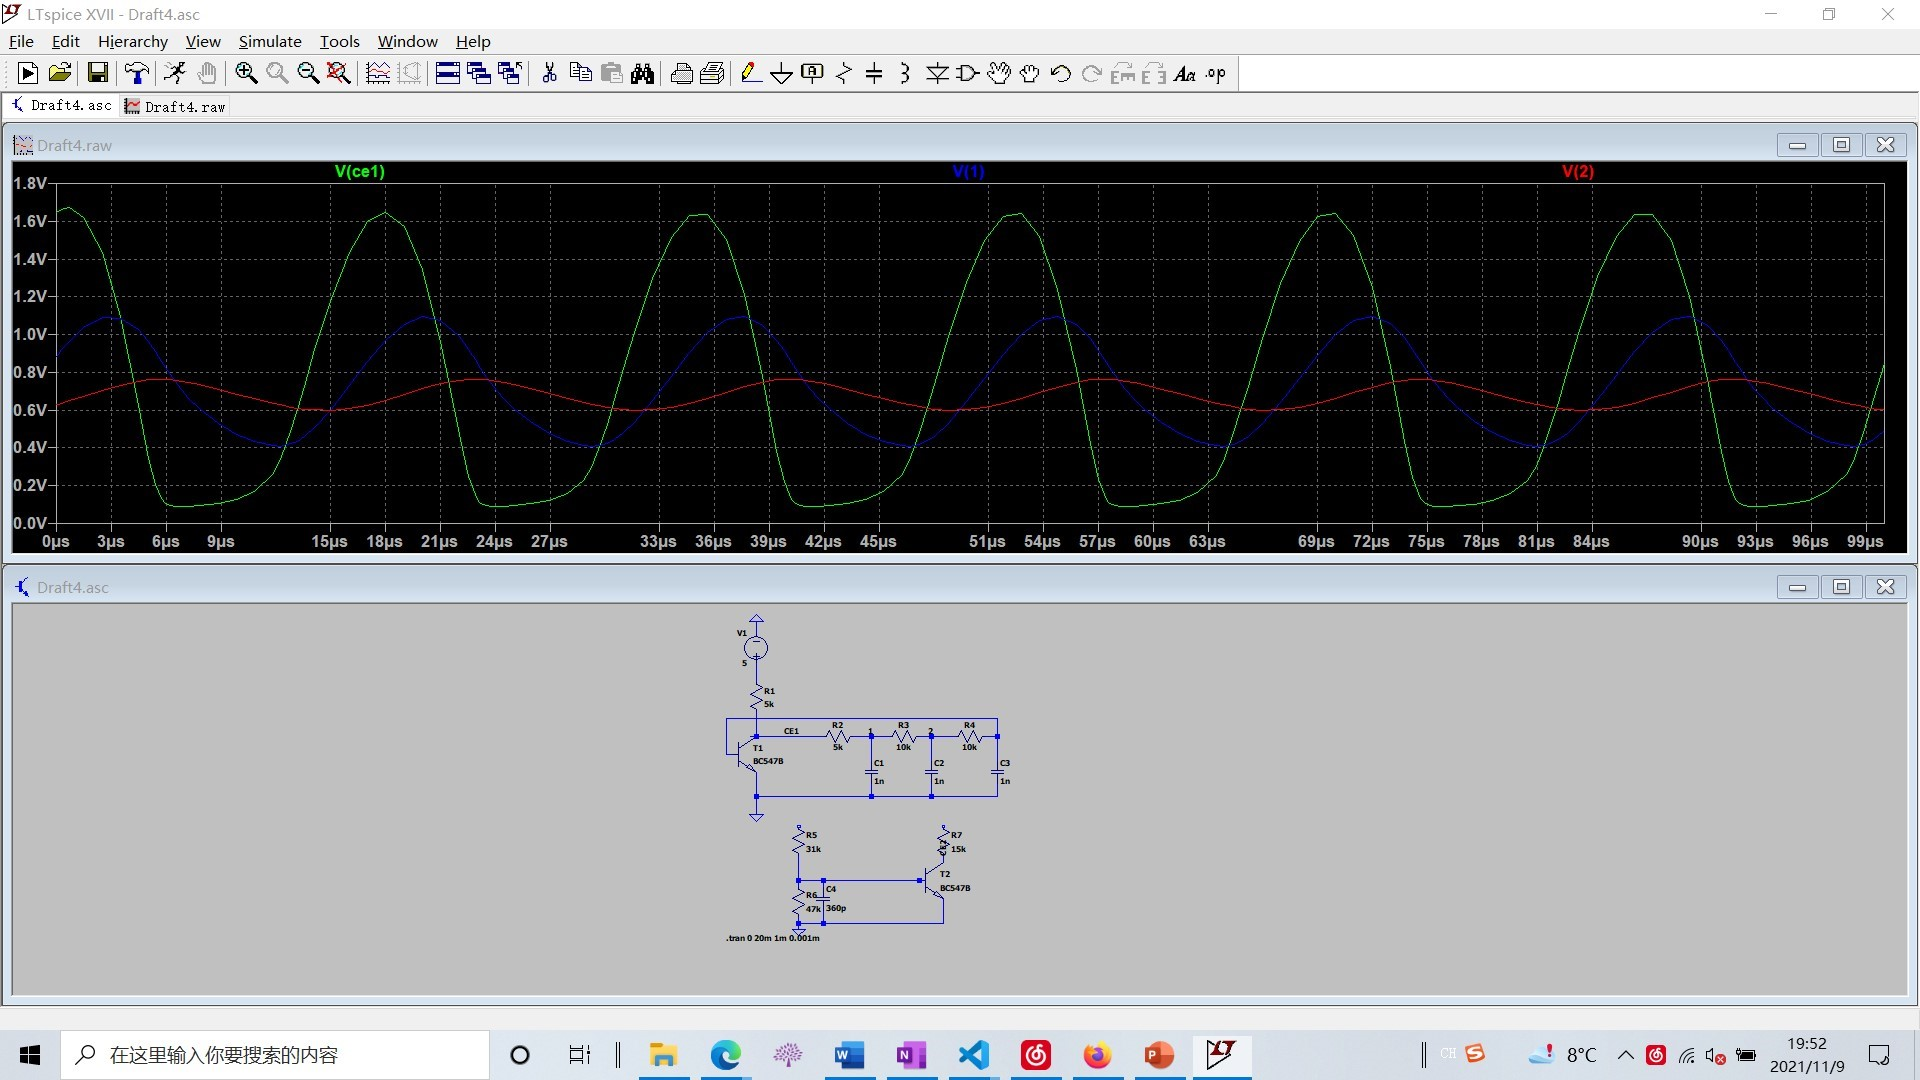
\includegraphics[width=0.60\textwidth]{1-1.jpg}
  \caption{1-1-仿真}
\end{figure}

接入电路图上方电路,可以测量$v_{CE1},v_1,v_2$的值,
记录实验波形如下图:
\begin{figure}[htbp]
    \centering
      \subfigure{
      \begin{minipage}[t]{0.50\linewidth}
      \centering
      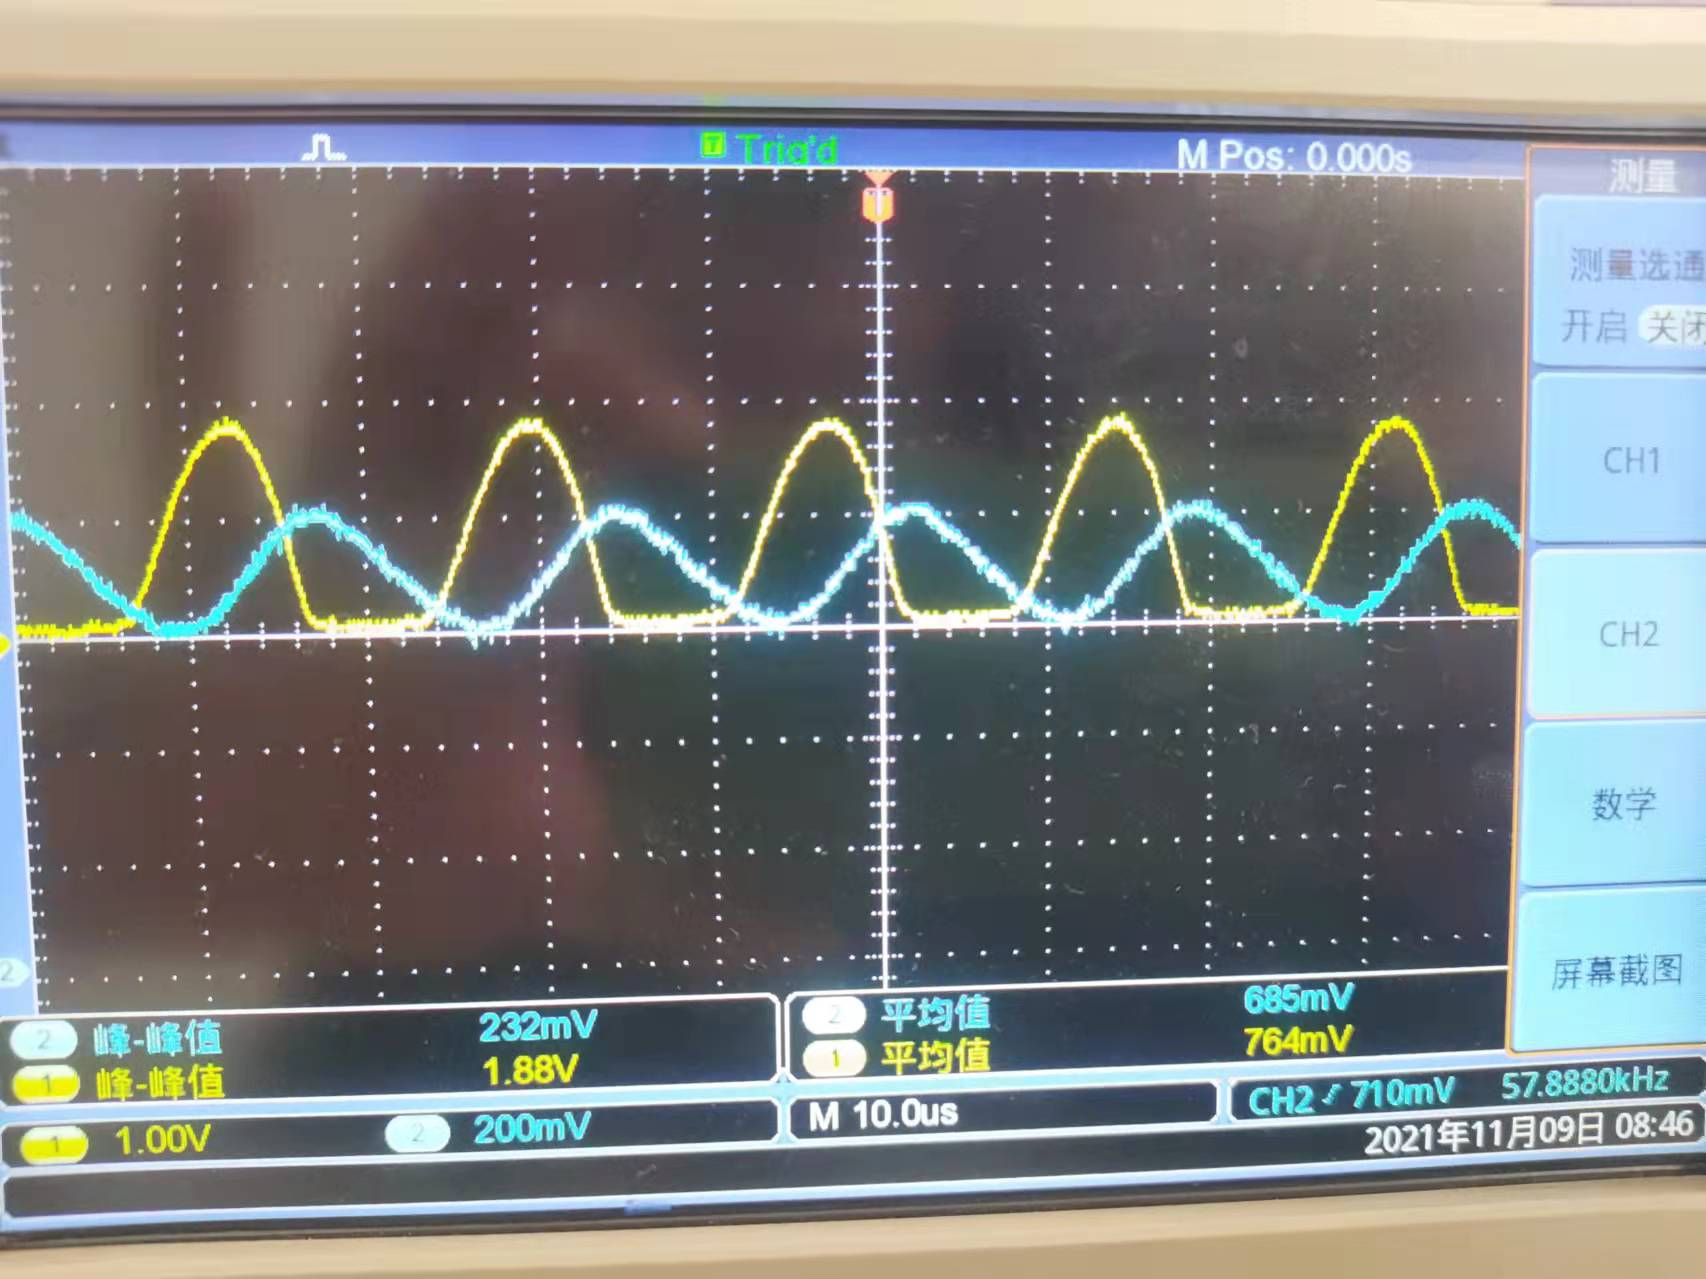
\includegraphics[width=3in]{1-1-ce1-1-r.jpg}
      \caption{$u_{ce1}(yellow),u_{1}(blue)$}
      \end{minipage}%
    }%
      \subfigure{
      \begin{minipage}[t]{0.50\linewidth}
      \centering
      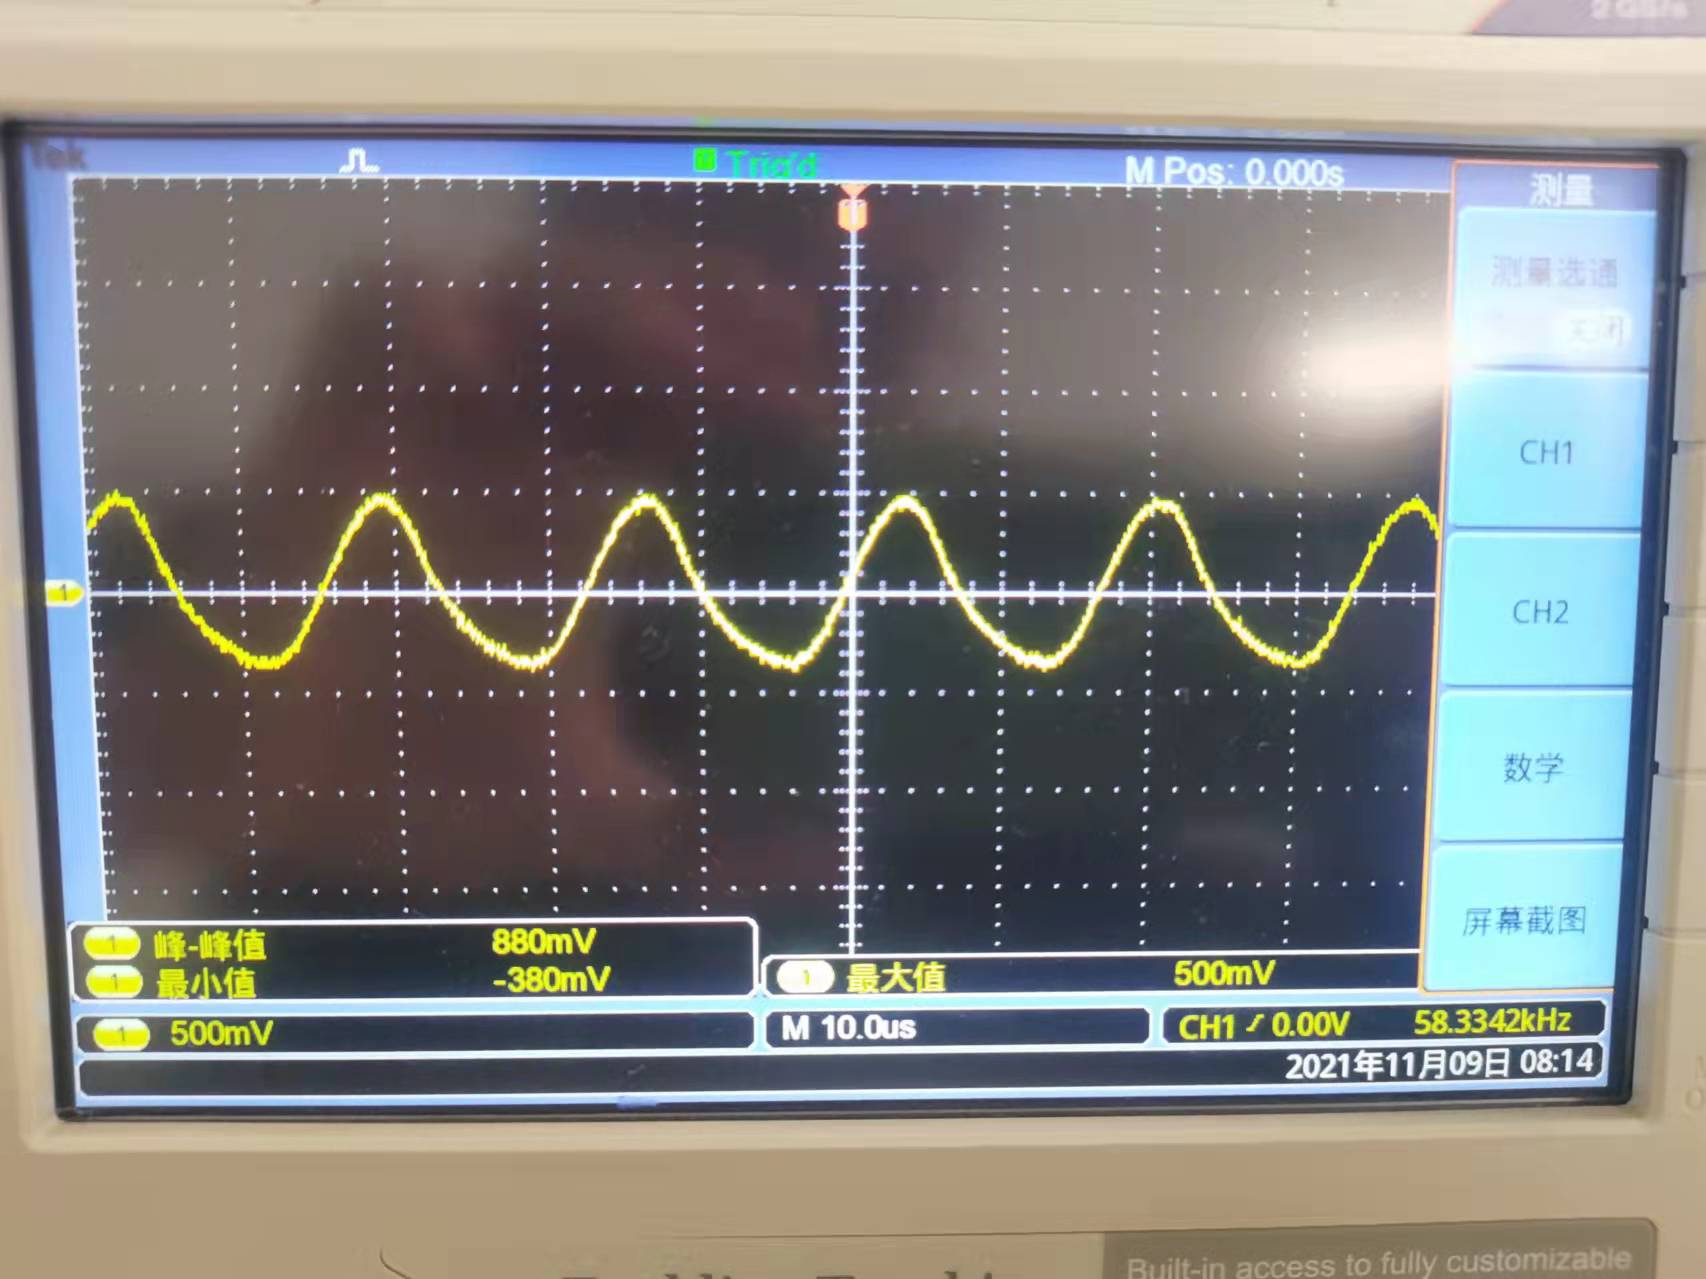
\includegraphics[width=3in]{1-1-2-r.jpg}
      \caption{$u_2$}
      \end{minipage}%
    }%
  
  \end{figure}

波形与仿真结果相近。

\subsubsection*{(2)接入虚线框内电路,调节 $R_5$,测量 $v_{CE1}$ 和 $v_{CE2}$ 波形,观察当 $R_5$ 约在
$31k \Omega$ 上下时的波形变化,并与仿真结果比较。}

对电路进行仿真,分别调整$R_5$从$29k \Omega$变化到$32k \Omega$,观察$u_{CE1},
u_{CE2}$的波形。
\begin{figure}[htbp]
  \centering
    \subfigure{
    \begin{minipage}[t]{0.33\linewidth}
    \centering
    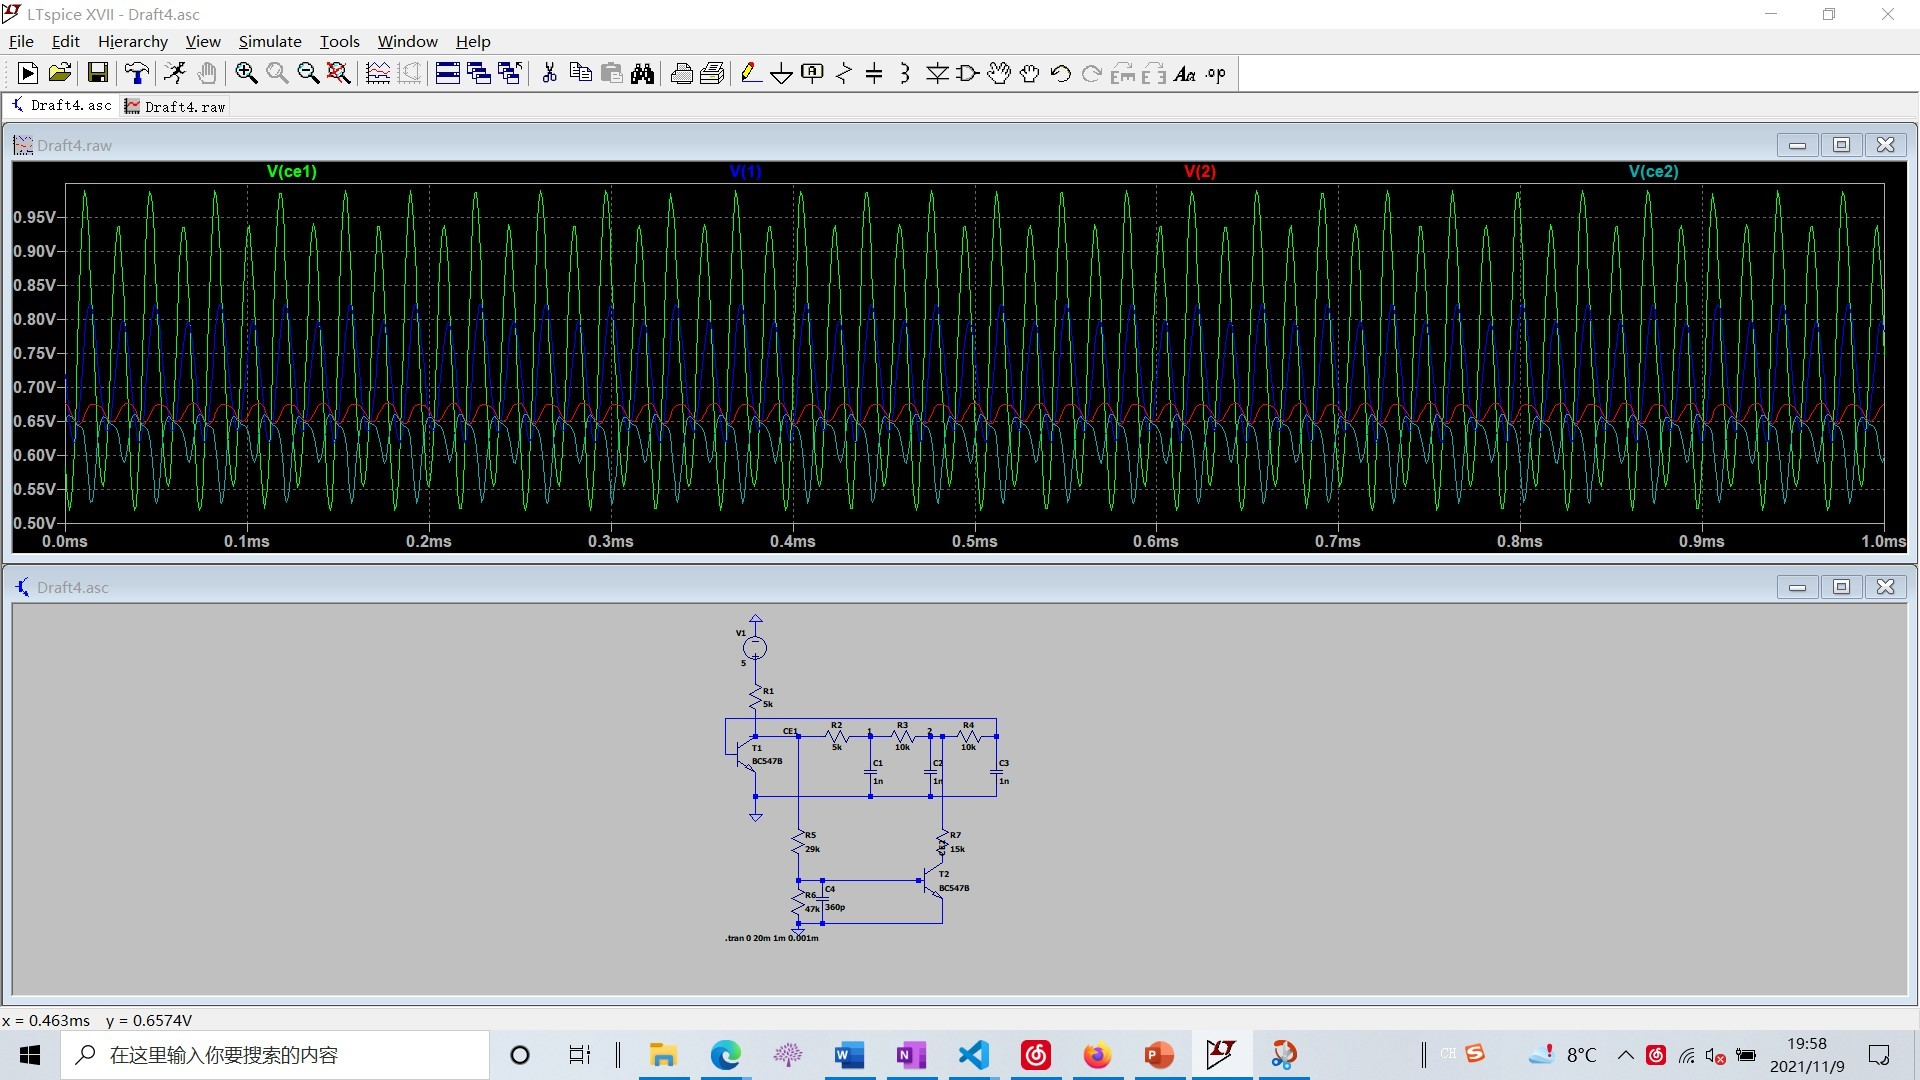
\includegraphics[width=2in]{1-2-29k.jpg}
    \caption{R5=29k}
    \end{minipage}%
  }%
    \subfigure{
    \begin{minipage}[t]{0.33\linewidth}
    \centering
    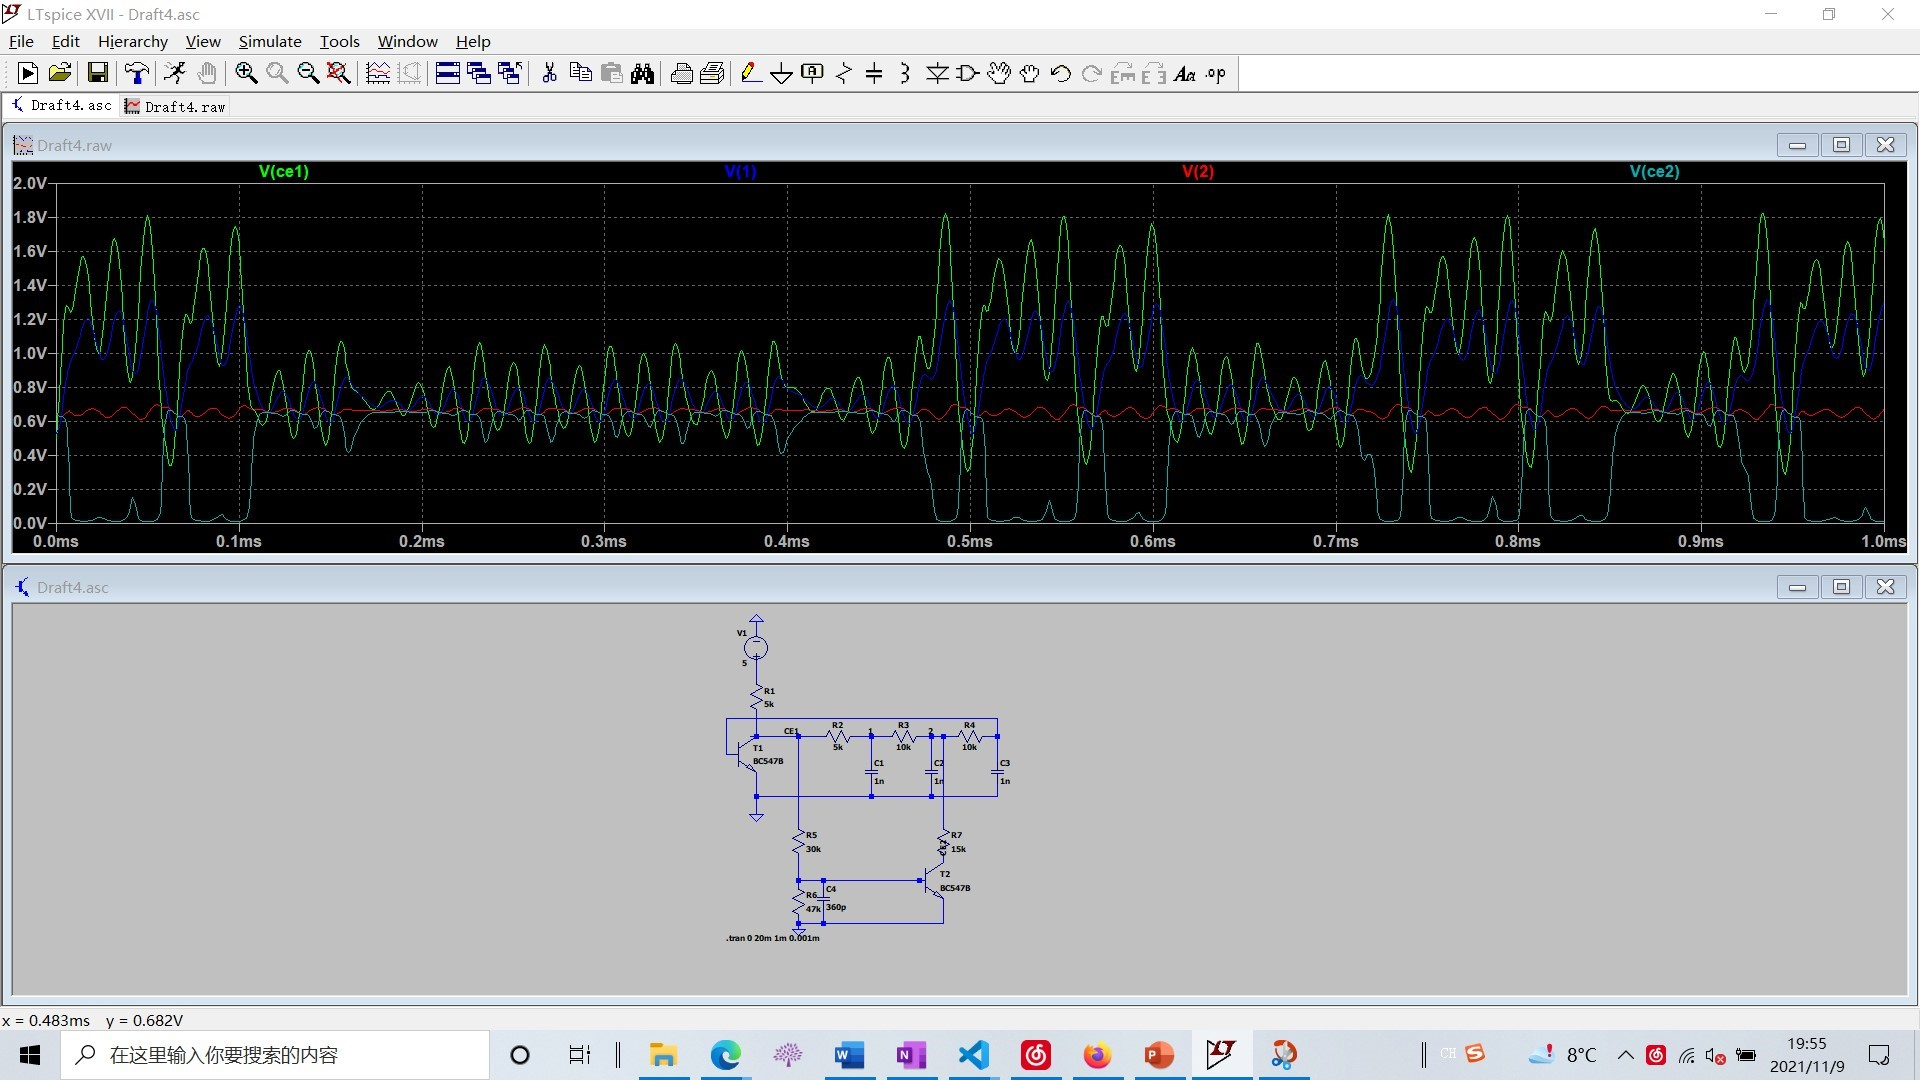
\includegraphics[width=2in]{1-2-30k.jpg}
    \caption{R5=30k}
    \end{minipage}%
  }%
  \subfigure{
    \begin{minipage}[t]{0.33\linewidth}
    \centering
    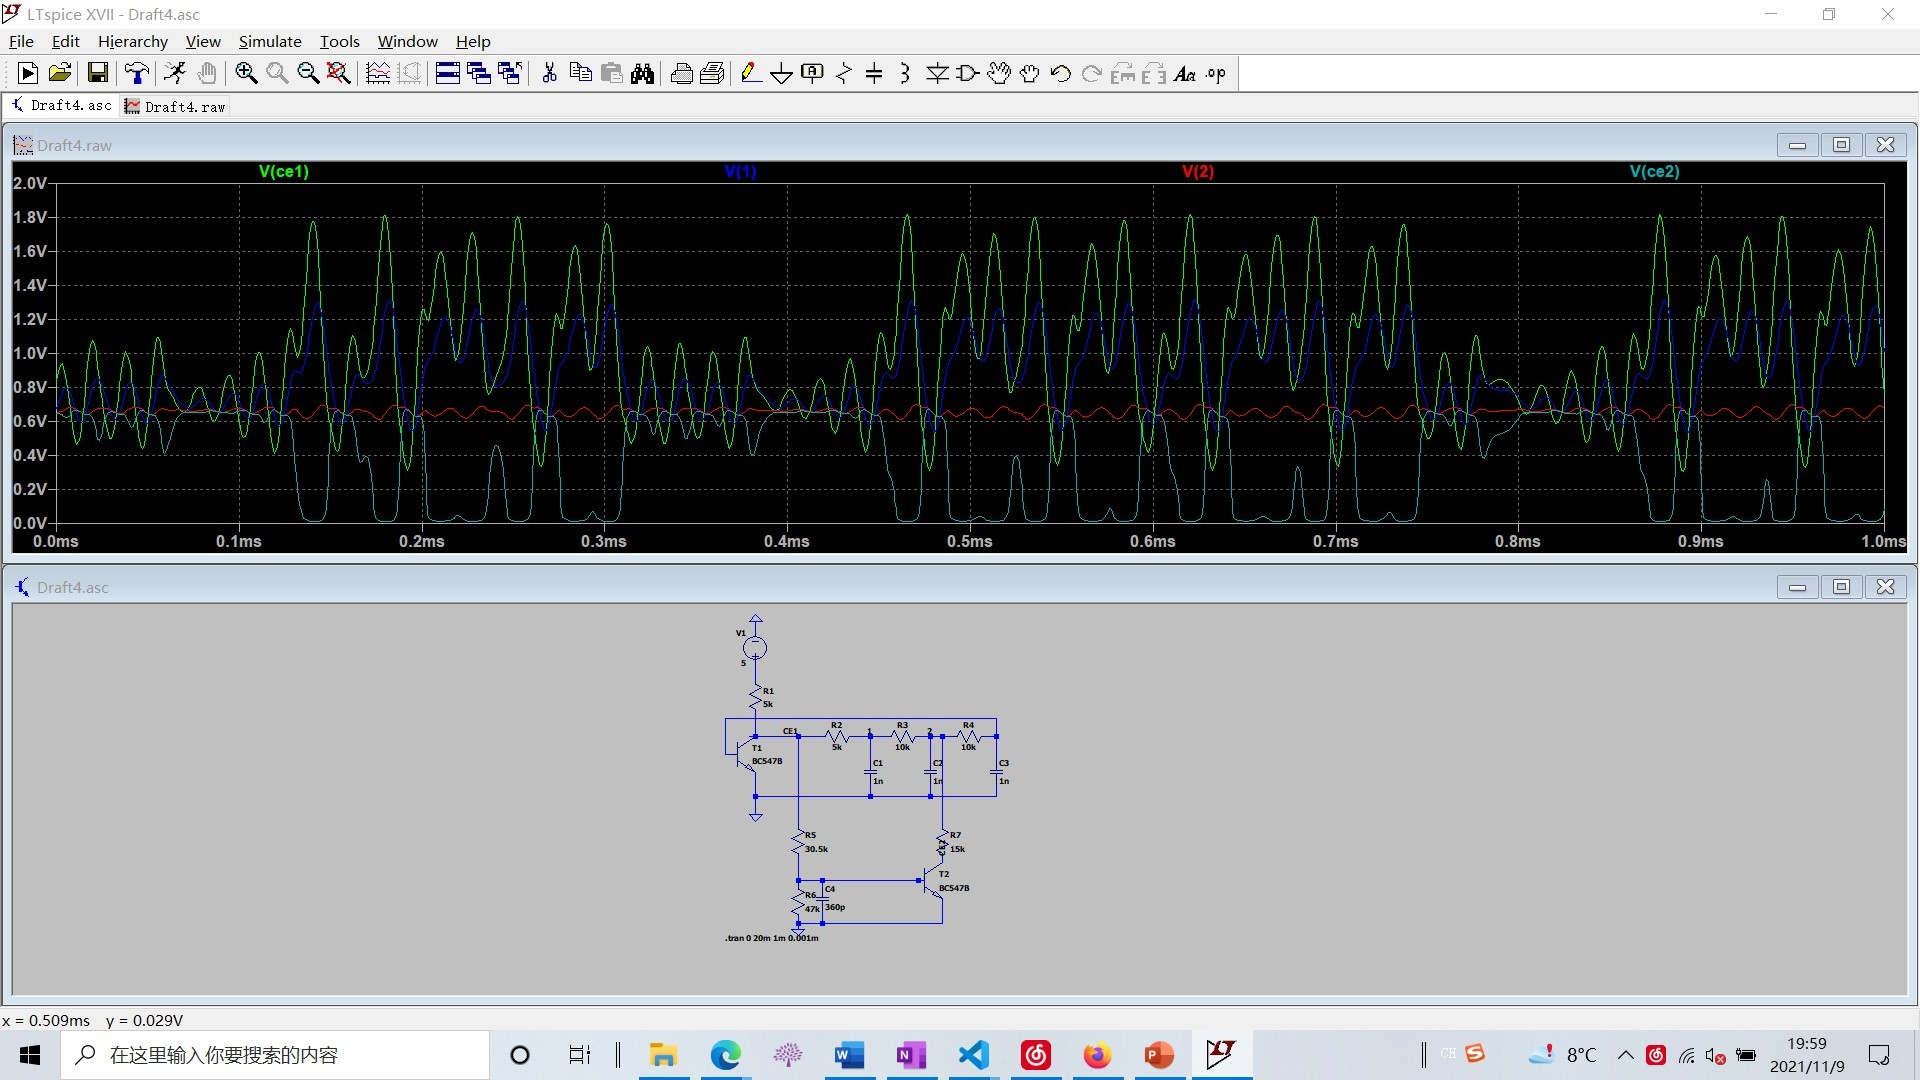
\includegraphics[width=2in]{1-2-30.5k.jpg}
    \caption{R5=30.5k}
    \end{minipage}%
  }%
\end{figure}

\begin{figure}[htbp]
  \centering
    \subfigure{
    \begin{minipage}[t]{0.33\linewidth}
    \centering
    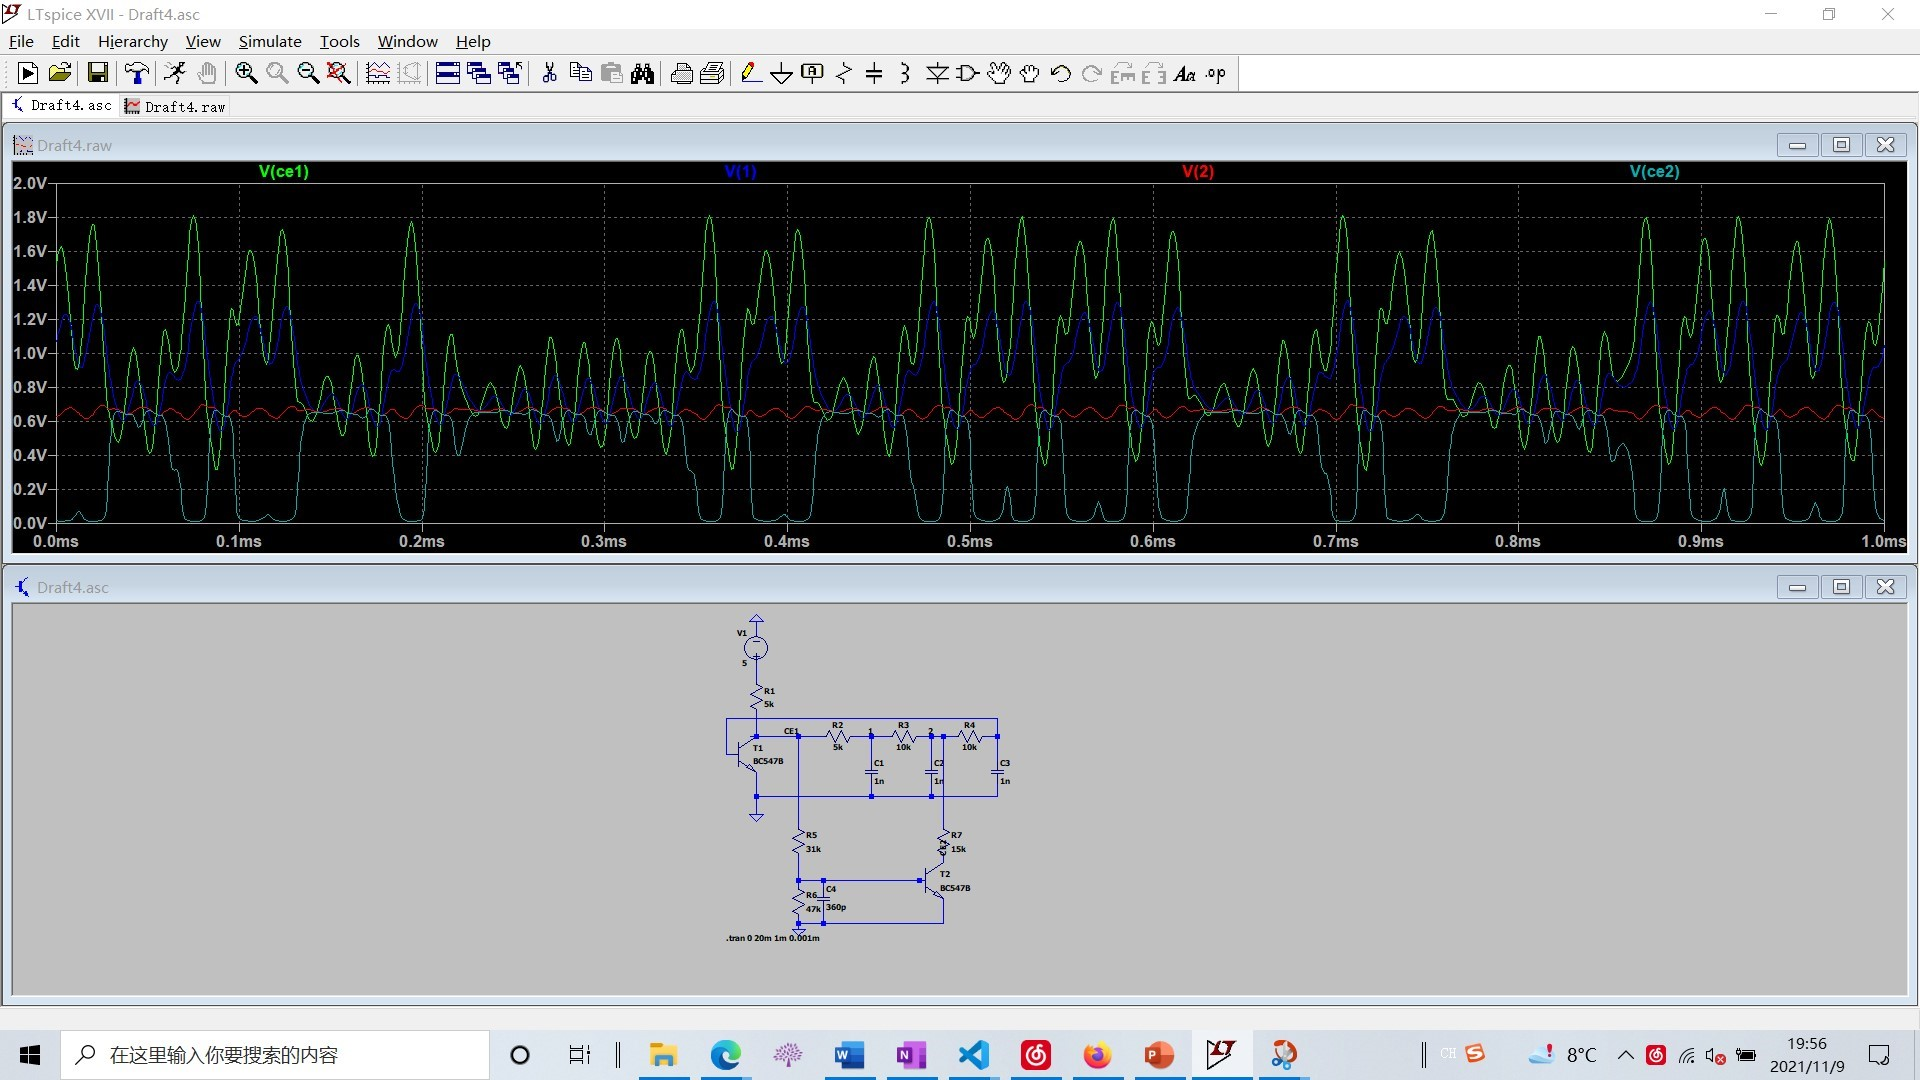
\includegraphics[width=2in]{1-2-31k.jpg}
    \caption{R5=31k}
    \end{minipage}%
  }%
    \subfigure{
    \begin{minipage}[t]{0.33\linewidth}
    \centering
    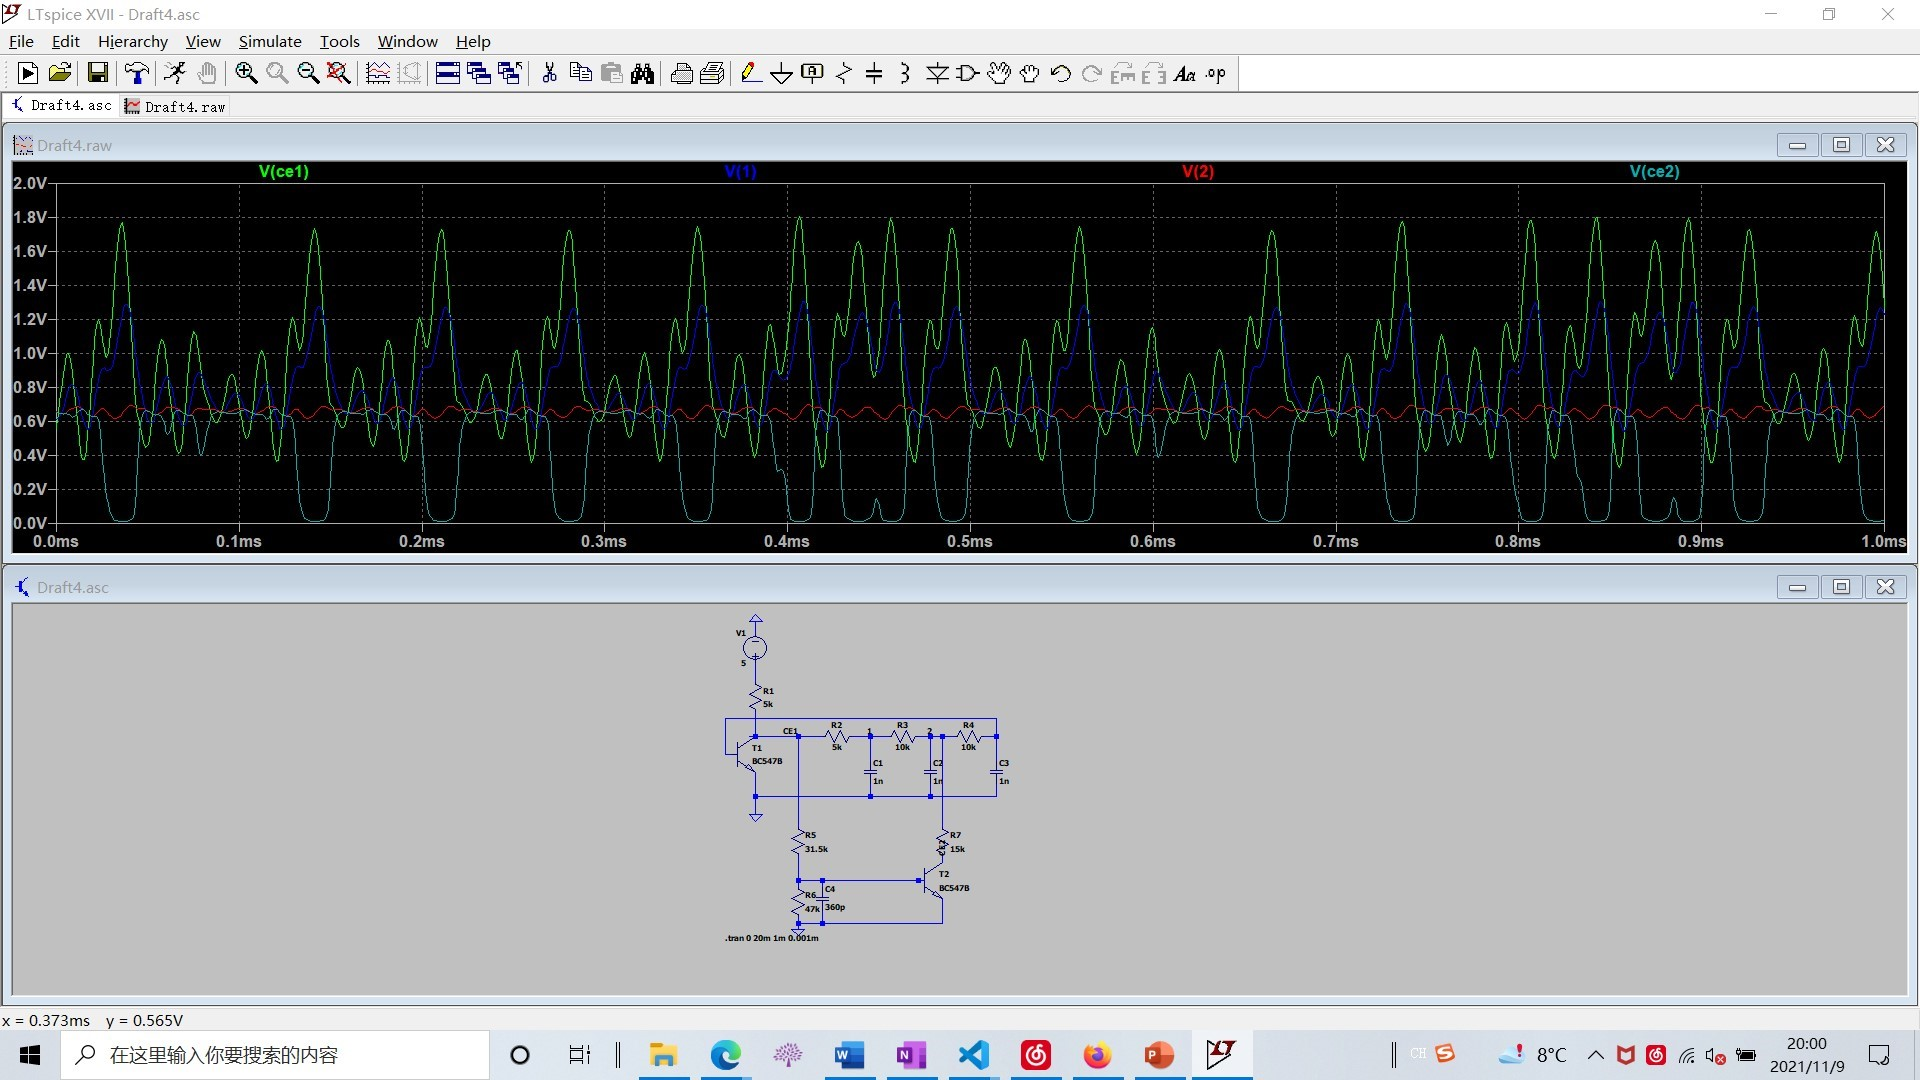
\includegraphics[width=2in]{1-2-31.5k.jpg}
    \caption{R5=31.5k}
    \end{minipage}%
  }%
  \subfigure{
    \begin{minipage}[t]{0.33\linewidth}
    \centering
    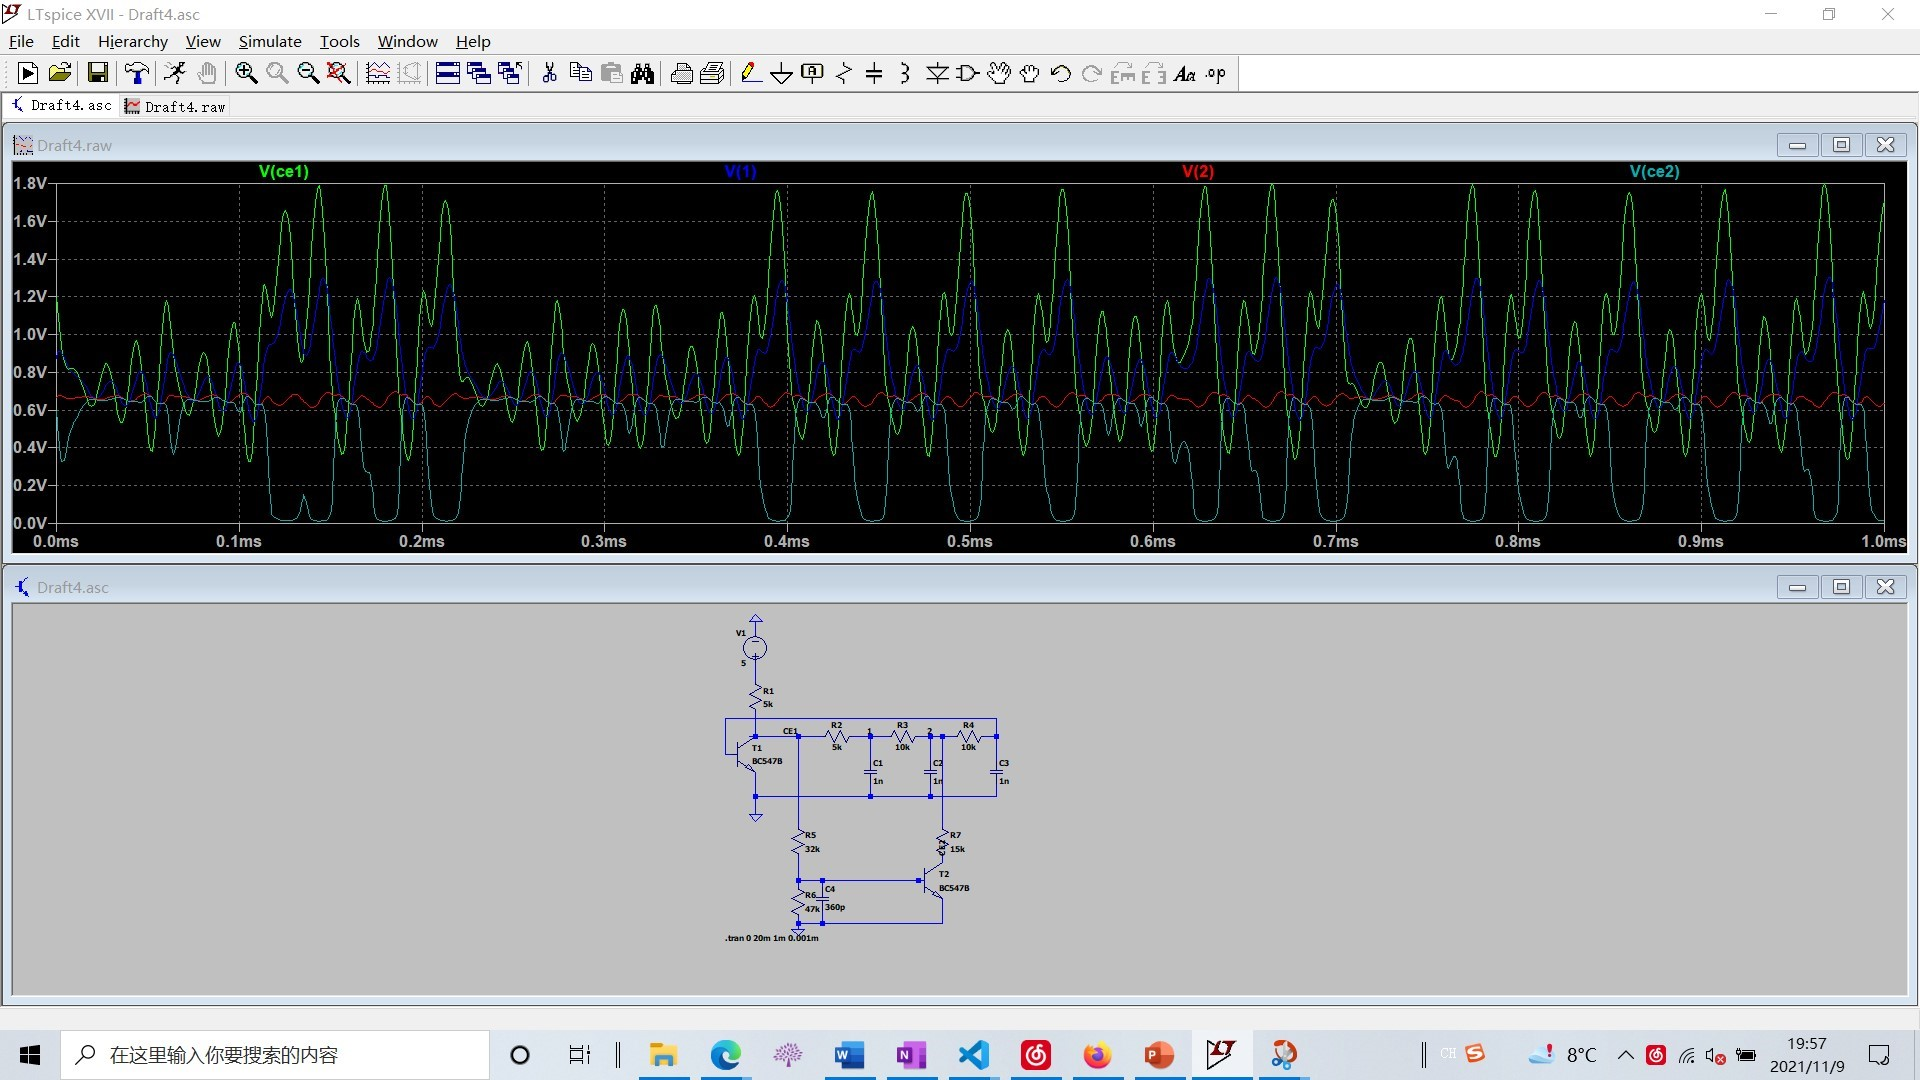
\includegraphics[width=2in]{1-2-32k.jpg}
    \caption{R5=32k}
    \end{minipage}%
  }%
\end{figure}

\newpage
实际搭建电路,调整可变电阻$R_5$从 $30 k \Omega$ 到 $32 k \Omega$,
记录示波器中$v_{CE1}$ 和 $v_{CE2}$的波形。

\begin{figure}[htbp]
  \centering
    \subfigure{
    \begin{minipage}[t]{0.33\linewidth}
    \centering
    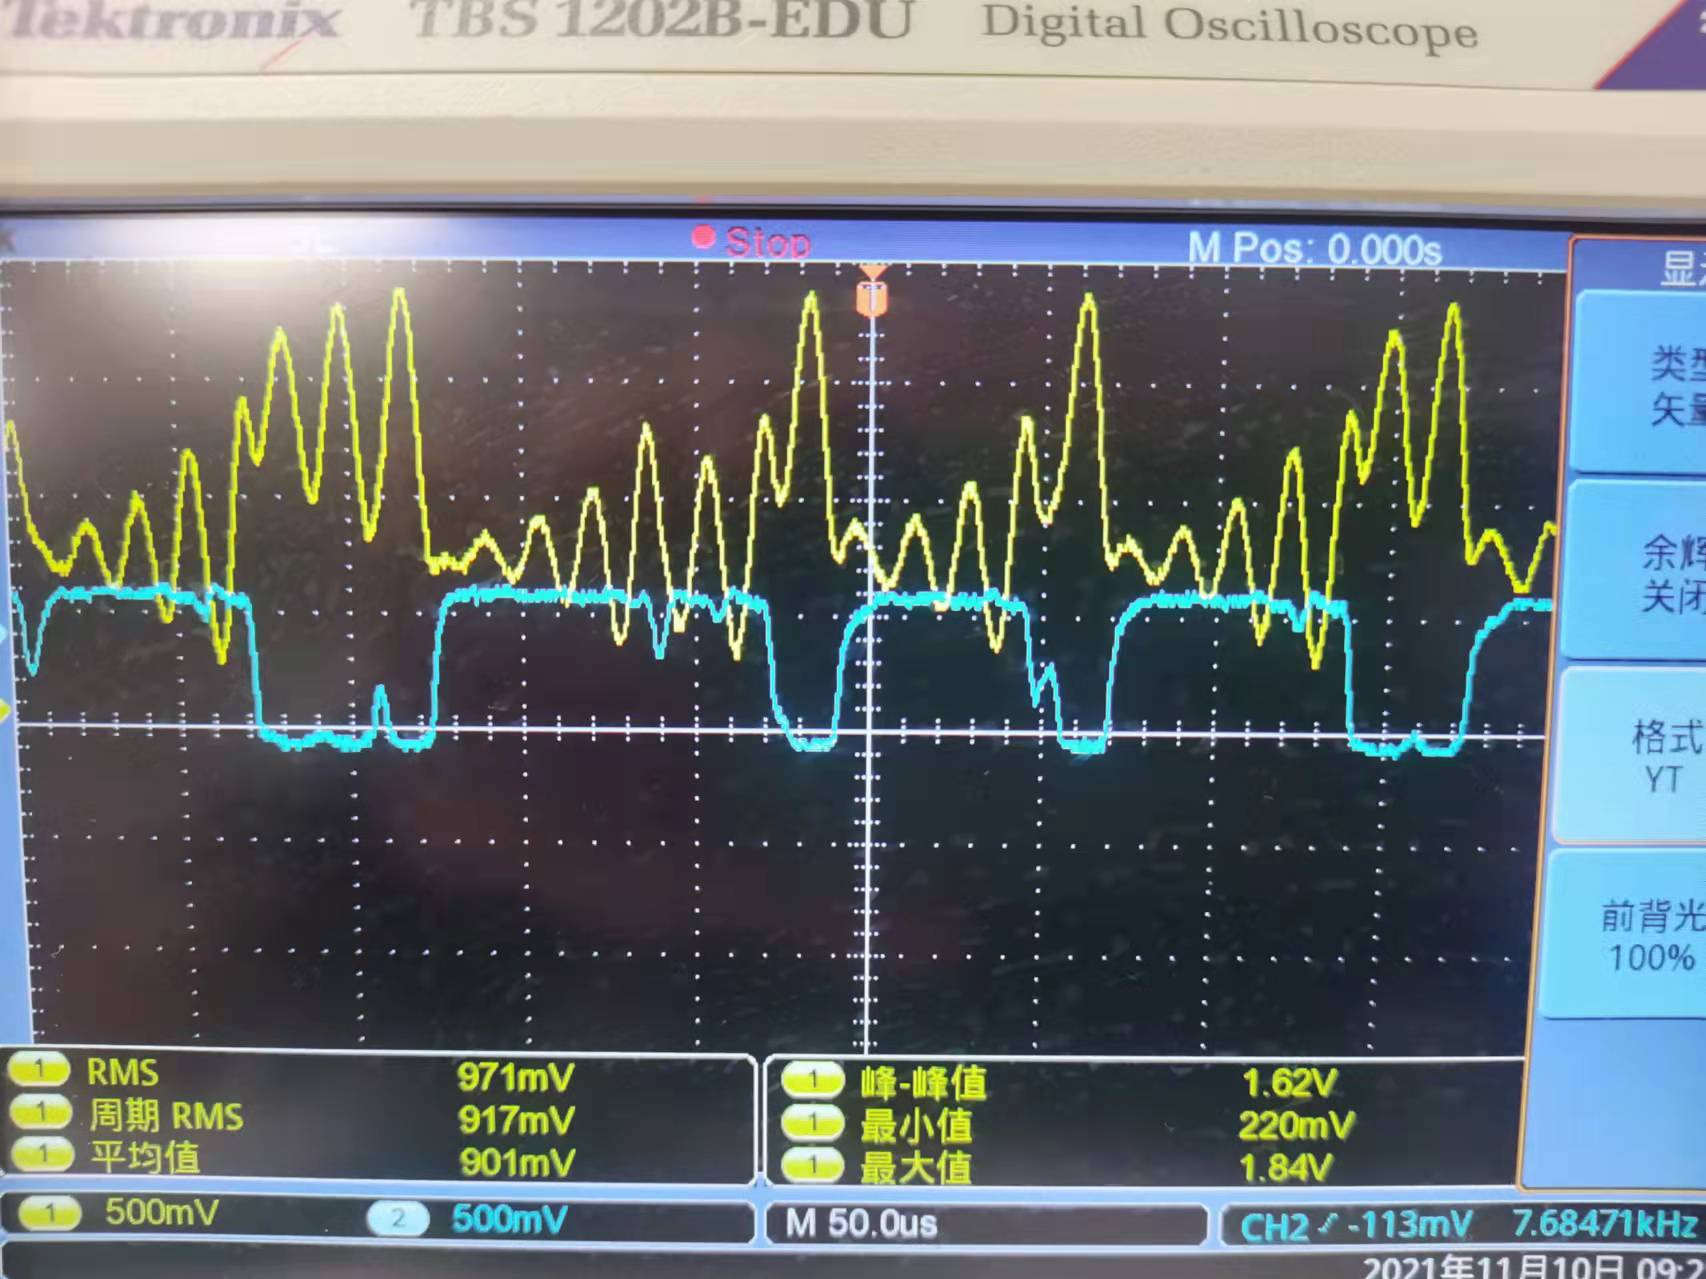
\includegraphics[width=2in]{1-2-30k-r.jpg}
    \caption{R5=30k}
    \end{minipage}%
  }%
  \subfigure{
    \begin{minipage}[t]{0.33\linewidth}
    \centering
    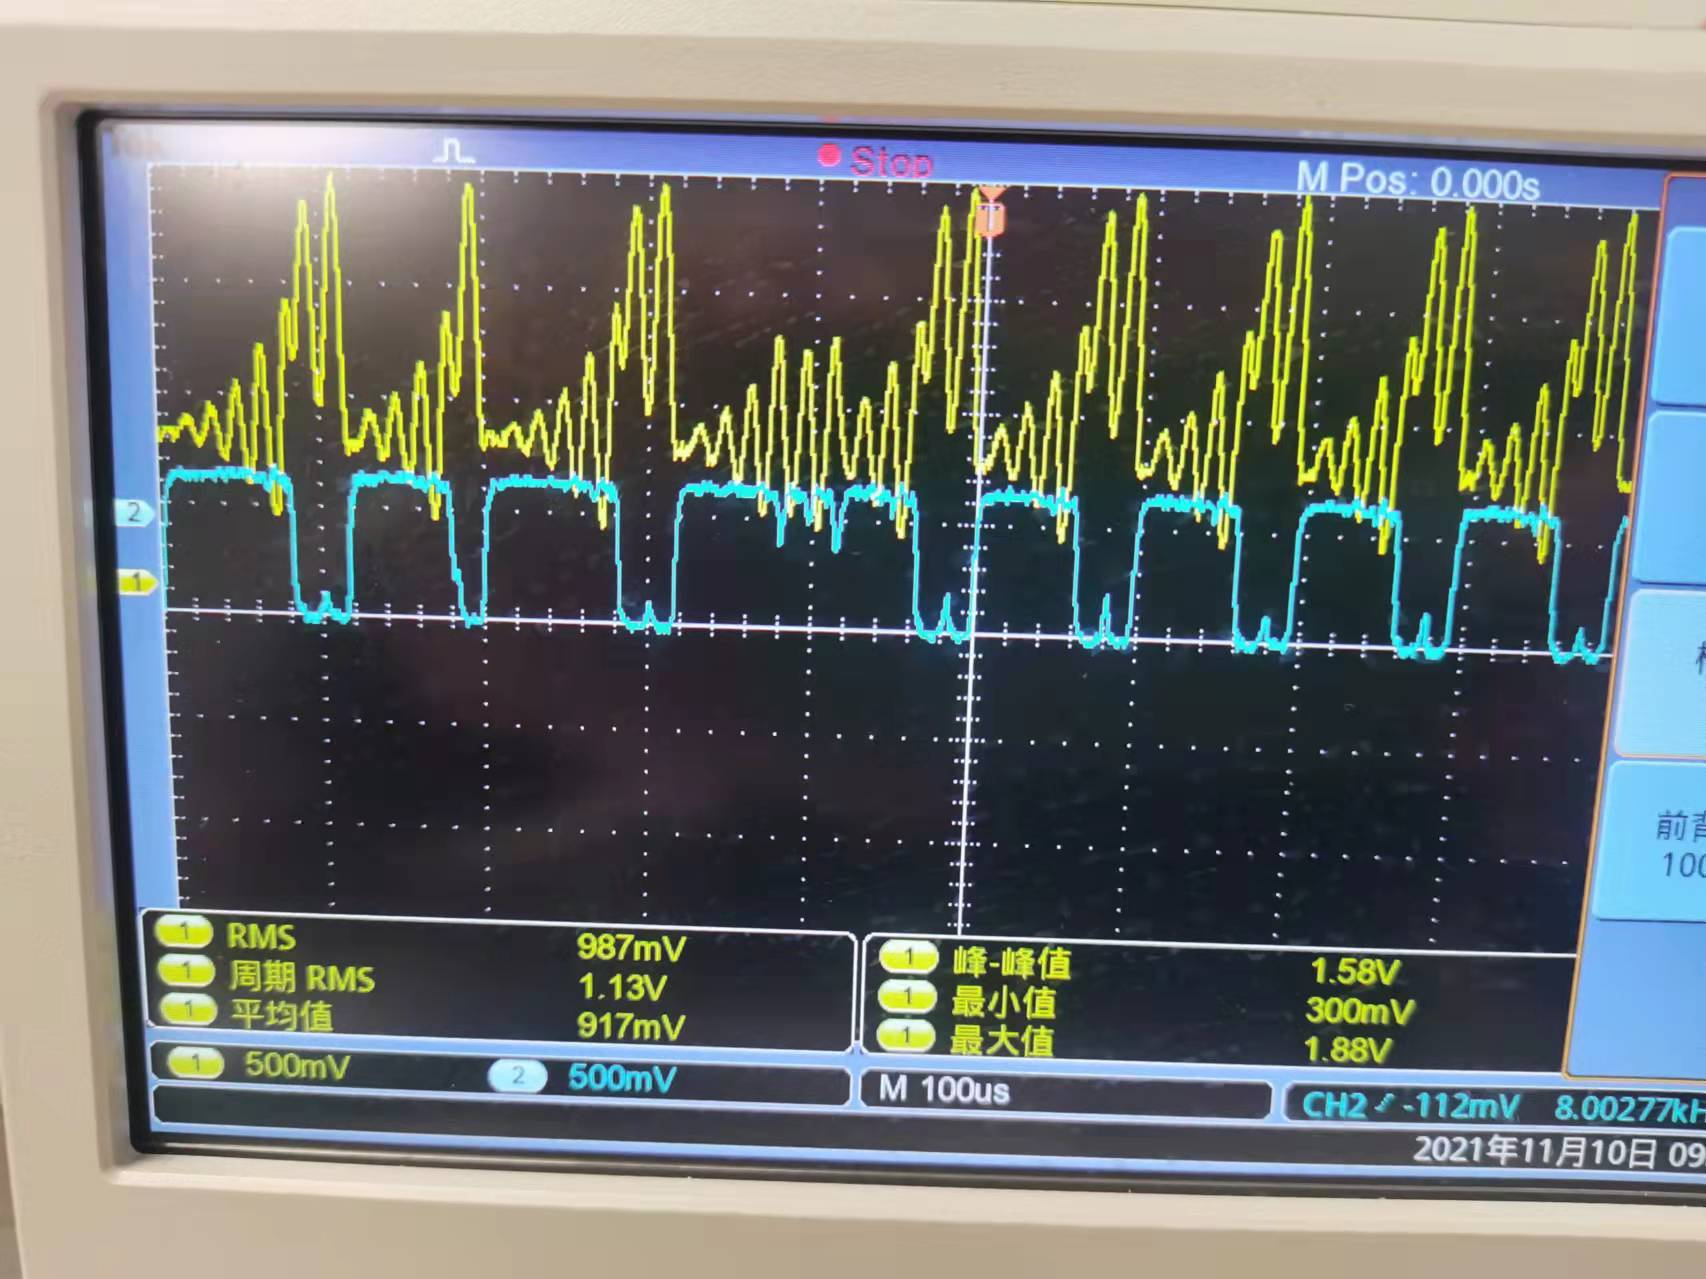
\includegraphics[width=2in]{1-2-30.5k-r.jpg}
    \caption{R5=30.5k}
    \end{minipage}%
  }%
\end{figure}
\begin{figure}[htbp]
  \centering
    \subfigure{
    \begin{minipage}[t]{0.33\linewidth}
    \centering
    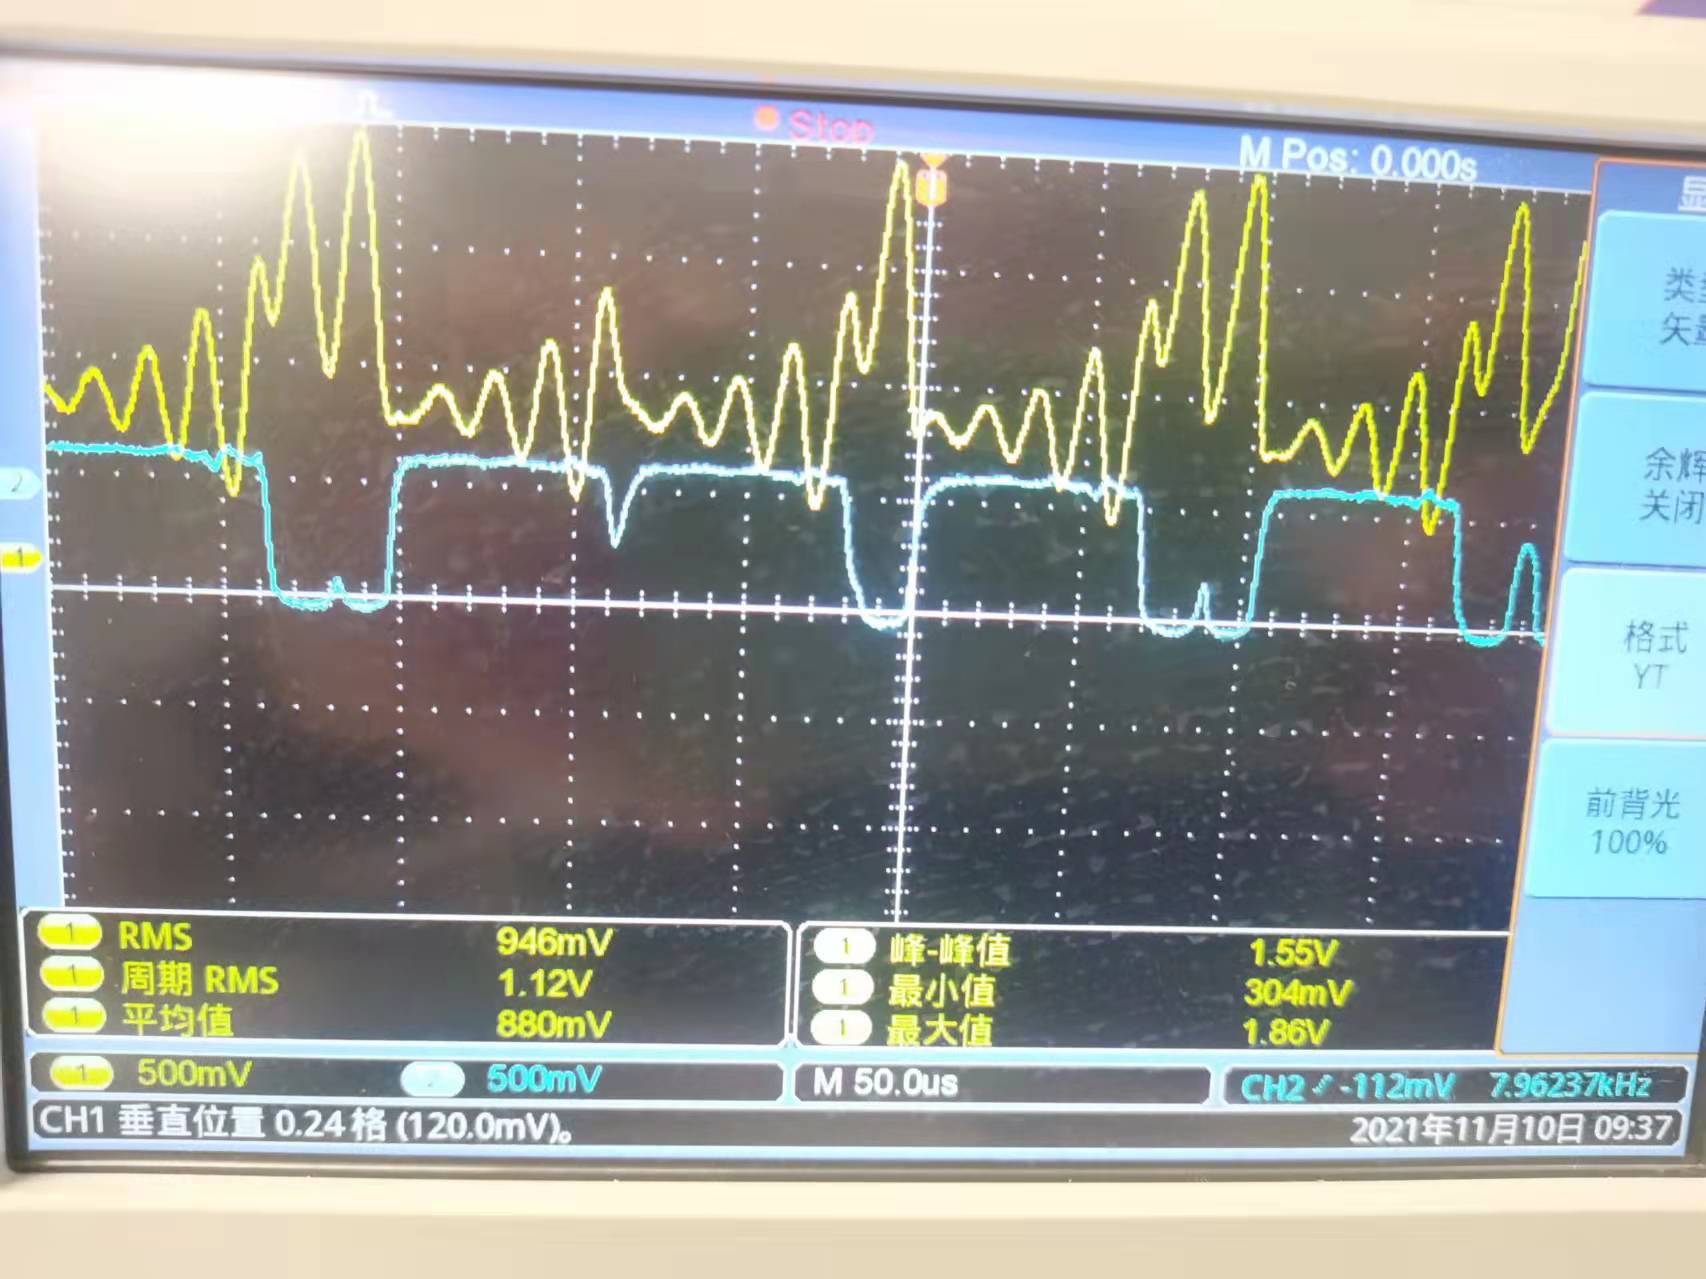
\includegraphics[width=2in]{1-2-31-r.jpg}
    \caption{R5=31k}
    \end{minipage}%
  }%
    \subfigure{
    \begin{minipage}[t]{0.33\linewidth}
    \centering
    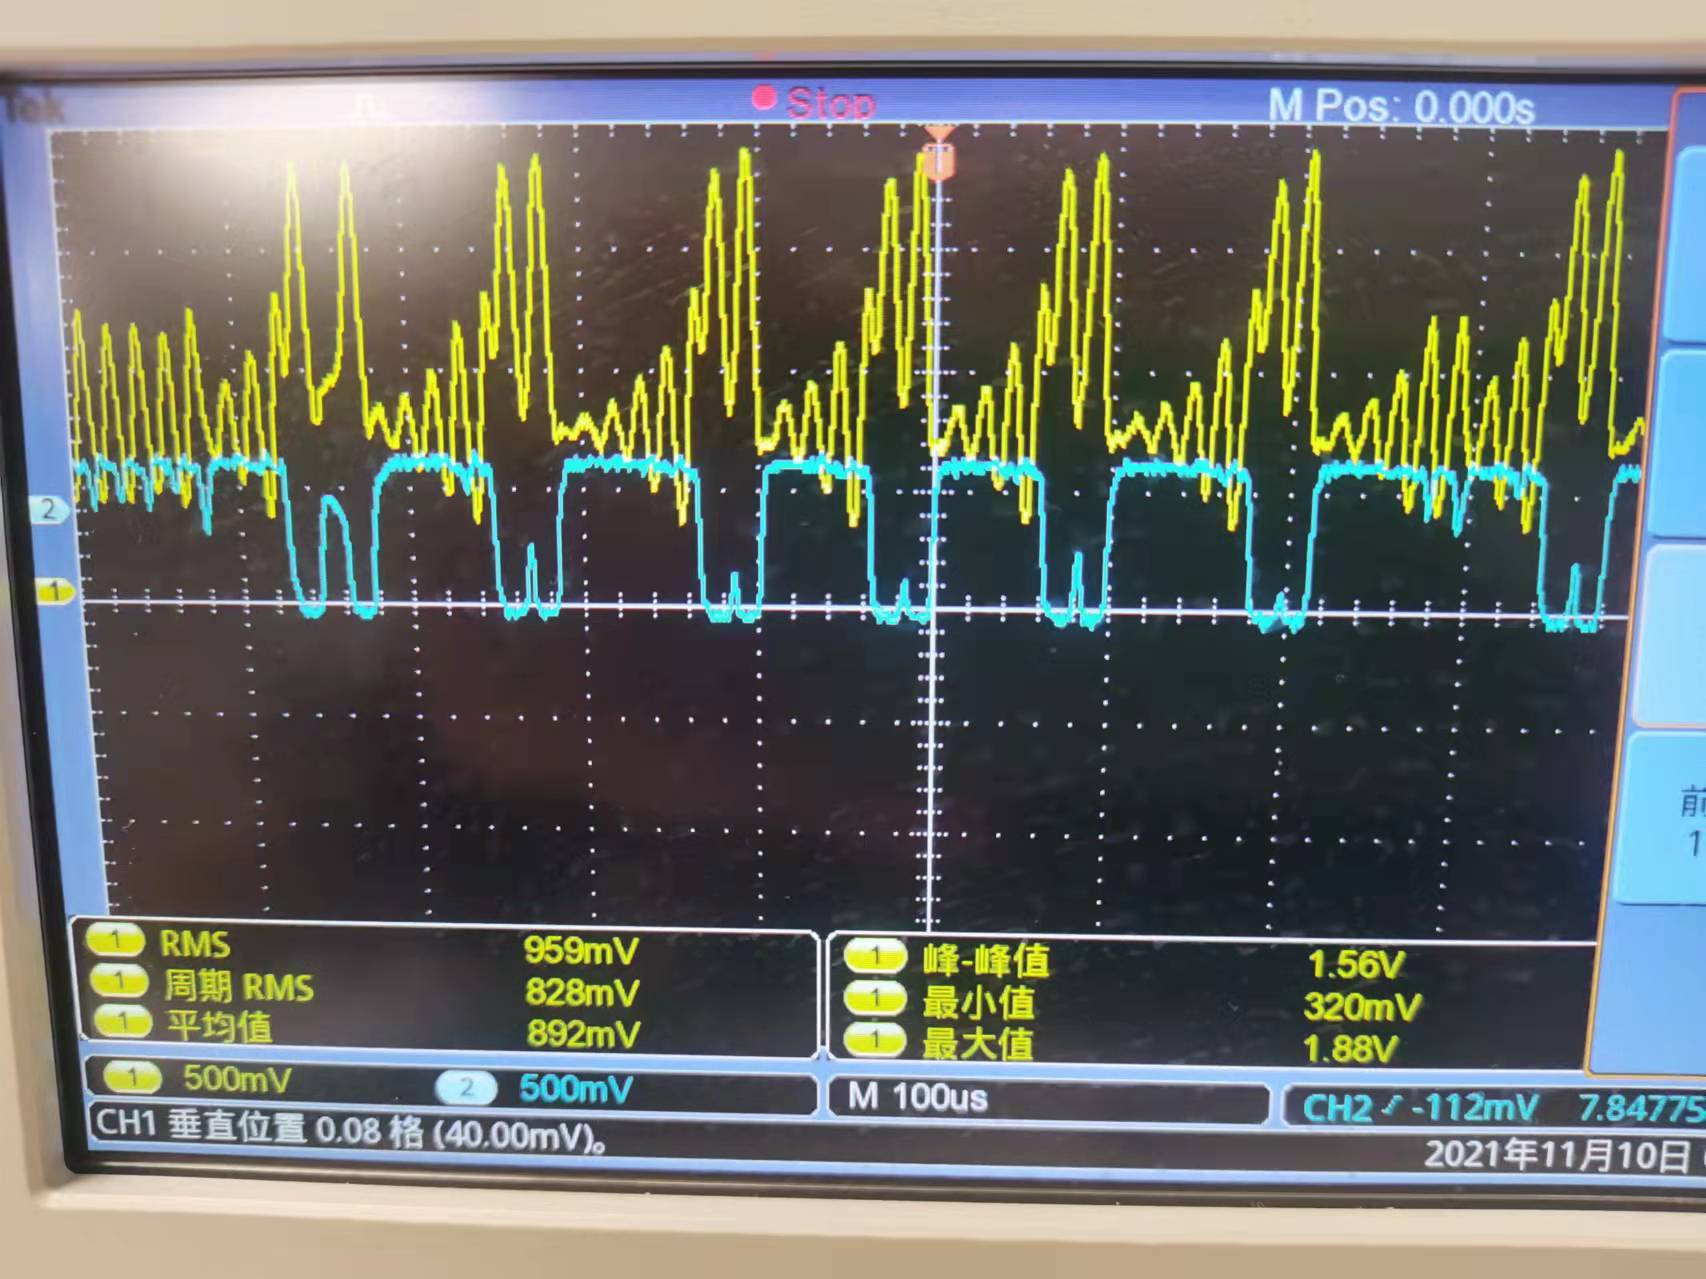
\includegraphics[width=2in]{1-2-31.5k-r.jpg}
    \caption{R5=31.5k}
    \end{minipage}%
  }%
  \subfigure{
    \begin{minipage}[t]{0.33\linewidth}
    \centering
    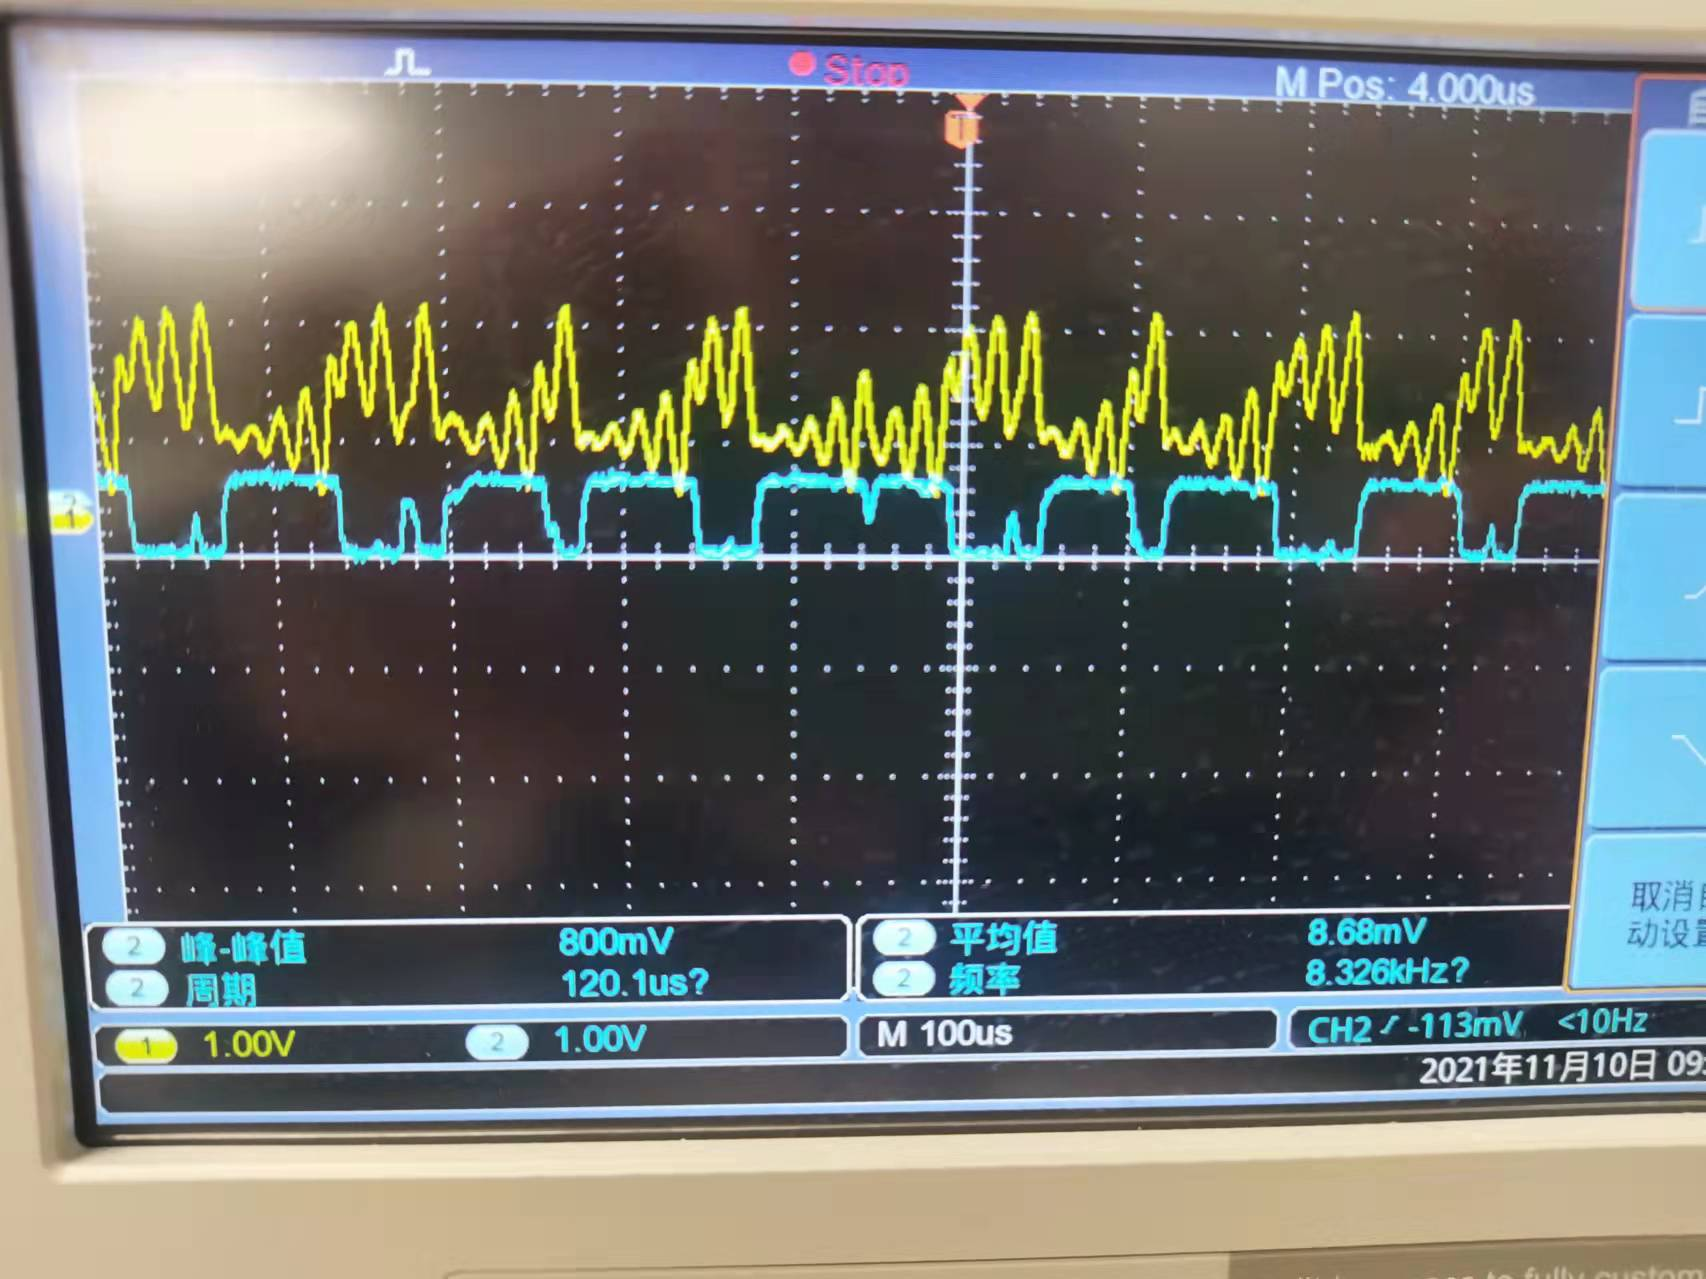
\includegraphics[width=2in]{1-2-32k-r.jpg}
    \caption{R5=32k}
    \end{minipage}%
  }%
\end{figure}

与仿真结果相比,$u_{CE2}$多了一部分负直流偏置,这可能是由
三极管的工作特性决定的。

\subsubsection*{
(3)用示波器 XY 显示模式(Utility->显示->格式->XY),调节 $R_5$ 阻值($31k \Omega$
上下),测量 $v_{CE1}$ 与 $v_{CE2}$,$v_{CE1}$ 与 v2,v1 与 v2的波形图,并与仿真结果比较。
}

先对电路进行仿真。

$R_5 = 30k \Omega$:

\begin{figure}[H]
  \centering
    \subfigure{
    \begin{minipage}[t]{0.33\linewidth}
    \centering
    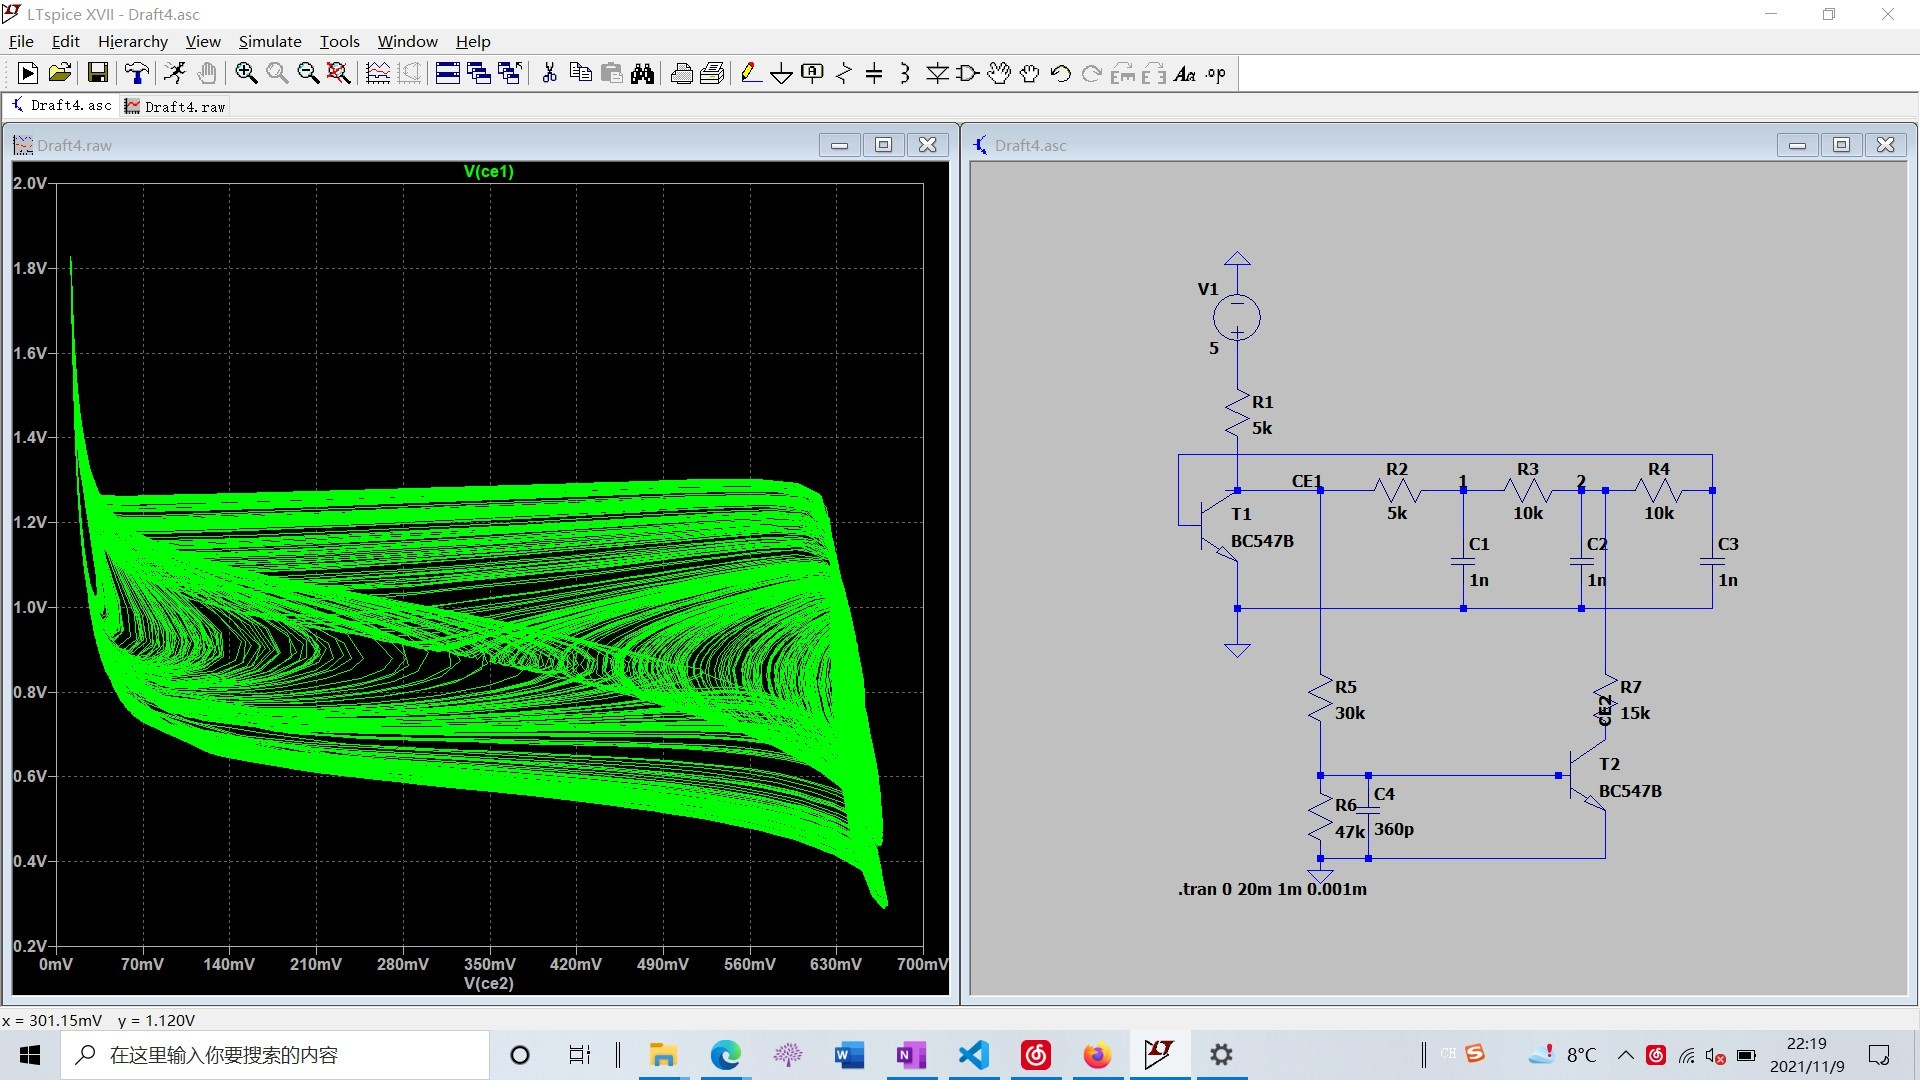
\includegraphics[width=2in]{1-3-30k-ce1ce2.jpg}
    \caption{$v_{CE1} - v_{CE2}$}
    \end{minipage}%
  }%
  \subfigure{
    \begin{minipage}[t]{0.33\linewidth}
    \centering
    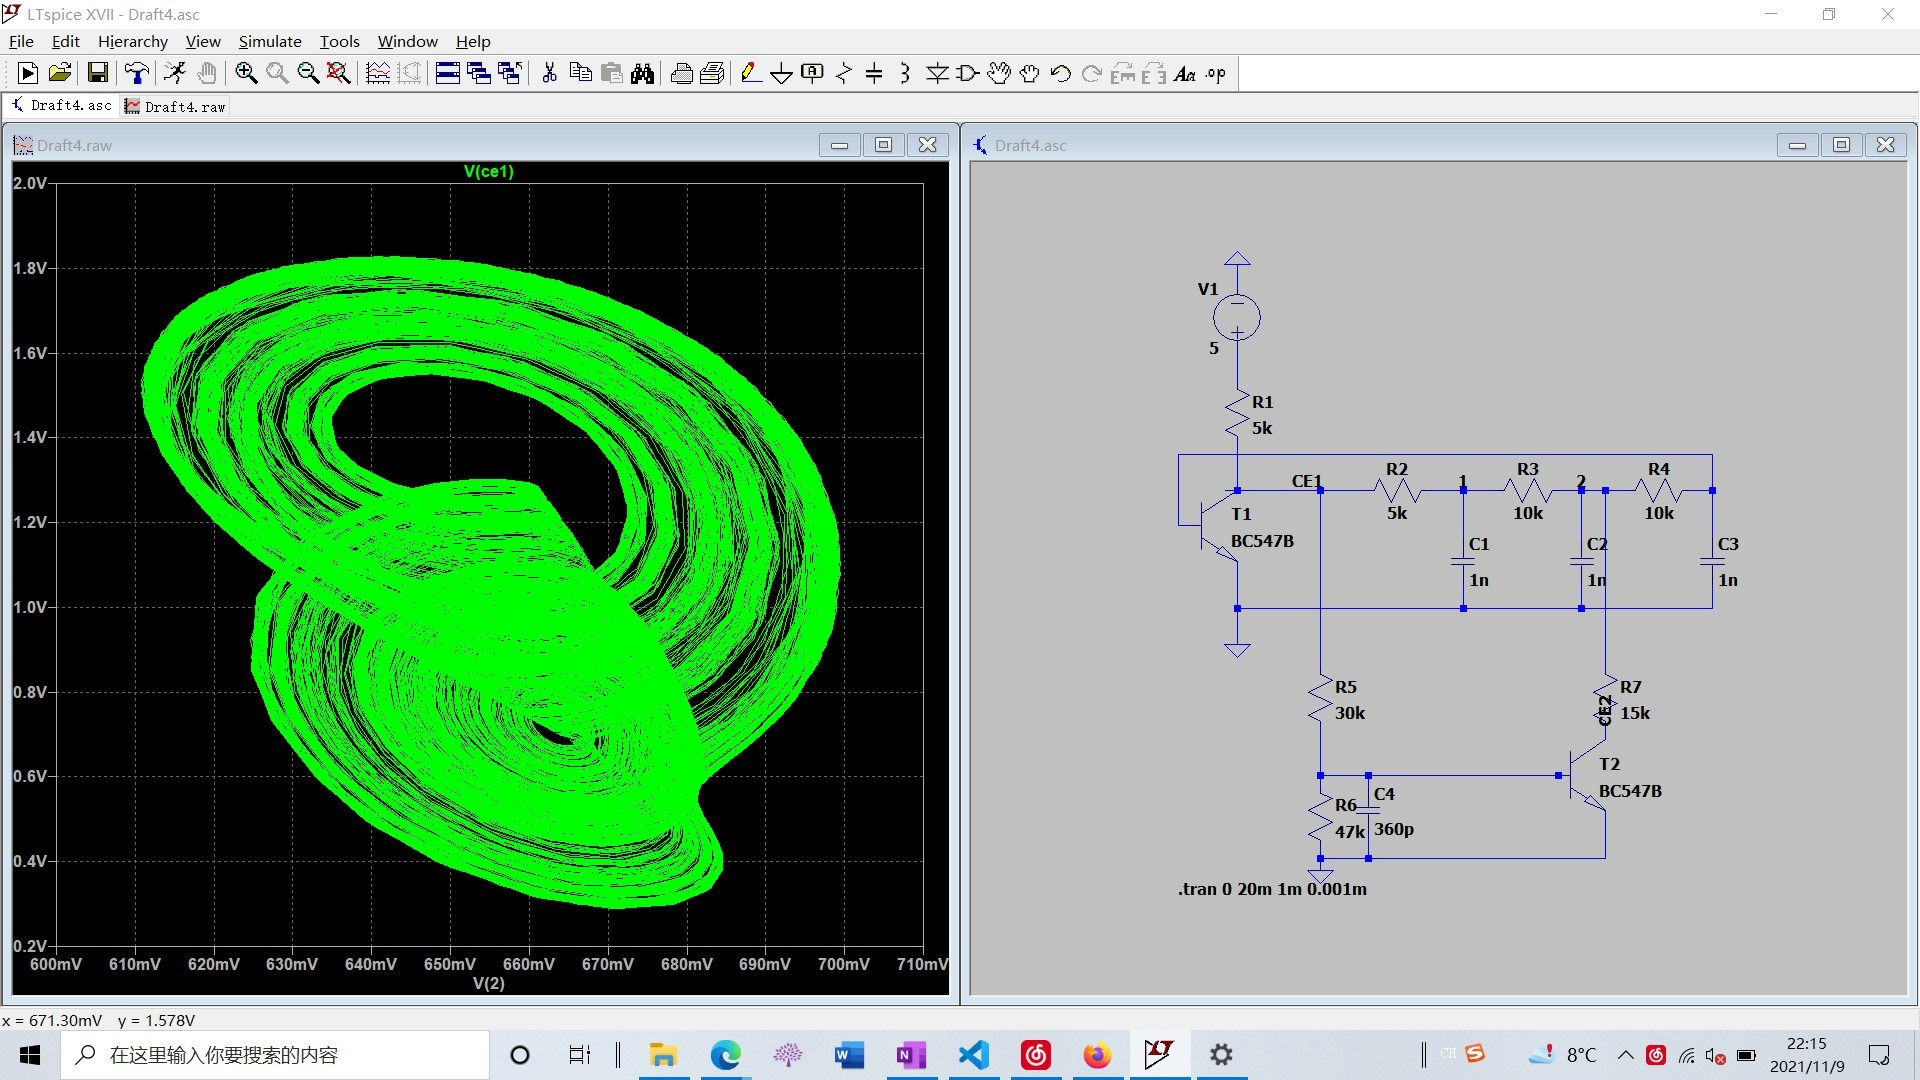
\includegraphics[width=2in]{1-3-30k-ce1-2.jpg}
    \caption{$v_{CE1} - v_{2}$}
    \end{minipage}%
  }%
  \subfigure{
    \begin{minipage}[t]{0.33\linewidth}
    \centering
    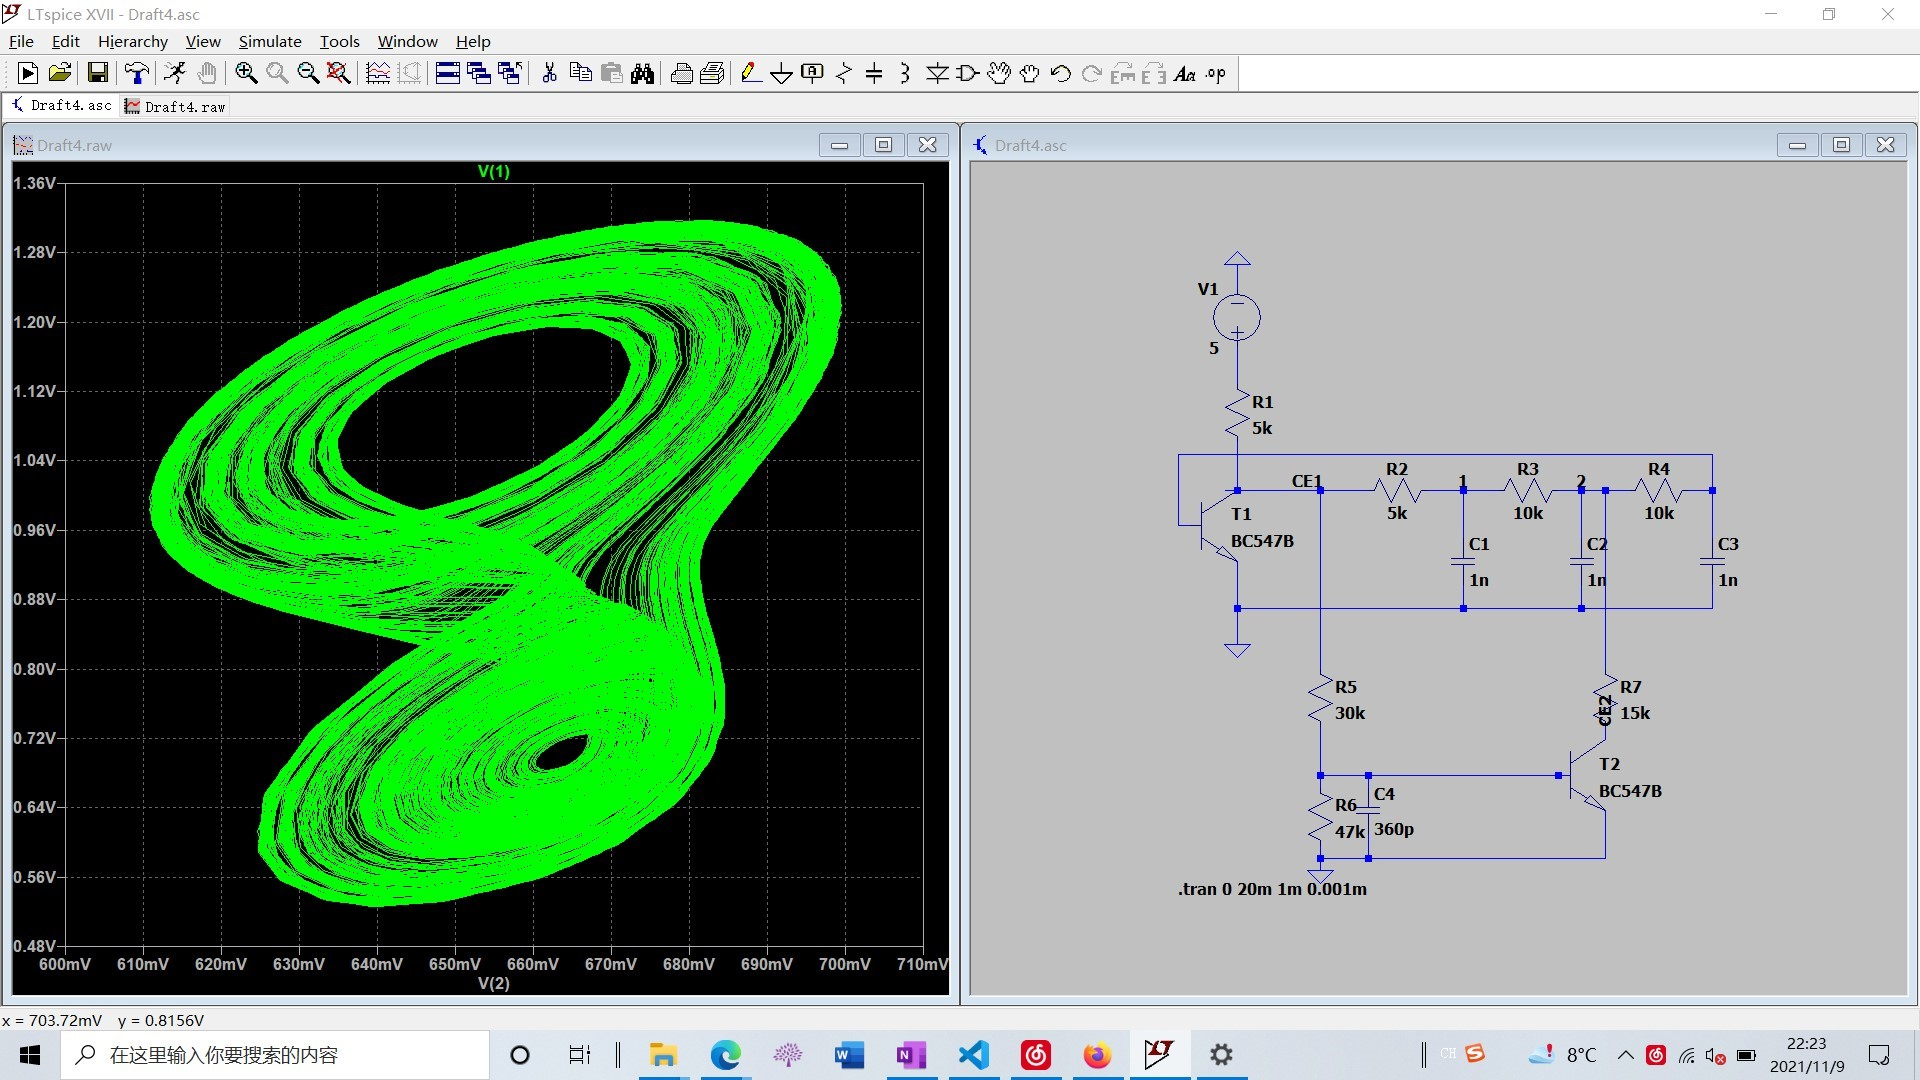
\includegraphics[width=2in]{1-3-30k-12.jpg}
    \caption{$v_{1} - v_{2}$}
    \end{minipage}%
  }%
  \end{figure}

  $R_5 = 30.5k \Omega$:

  \begin{figure}[H]
    \centering
      \subfigure{
      \begin{minipage}[t]{0.33\linewidth}
      \centering
      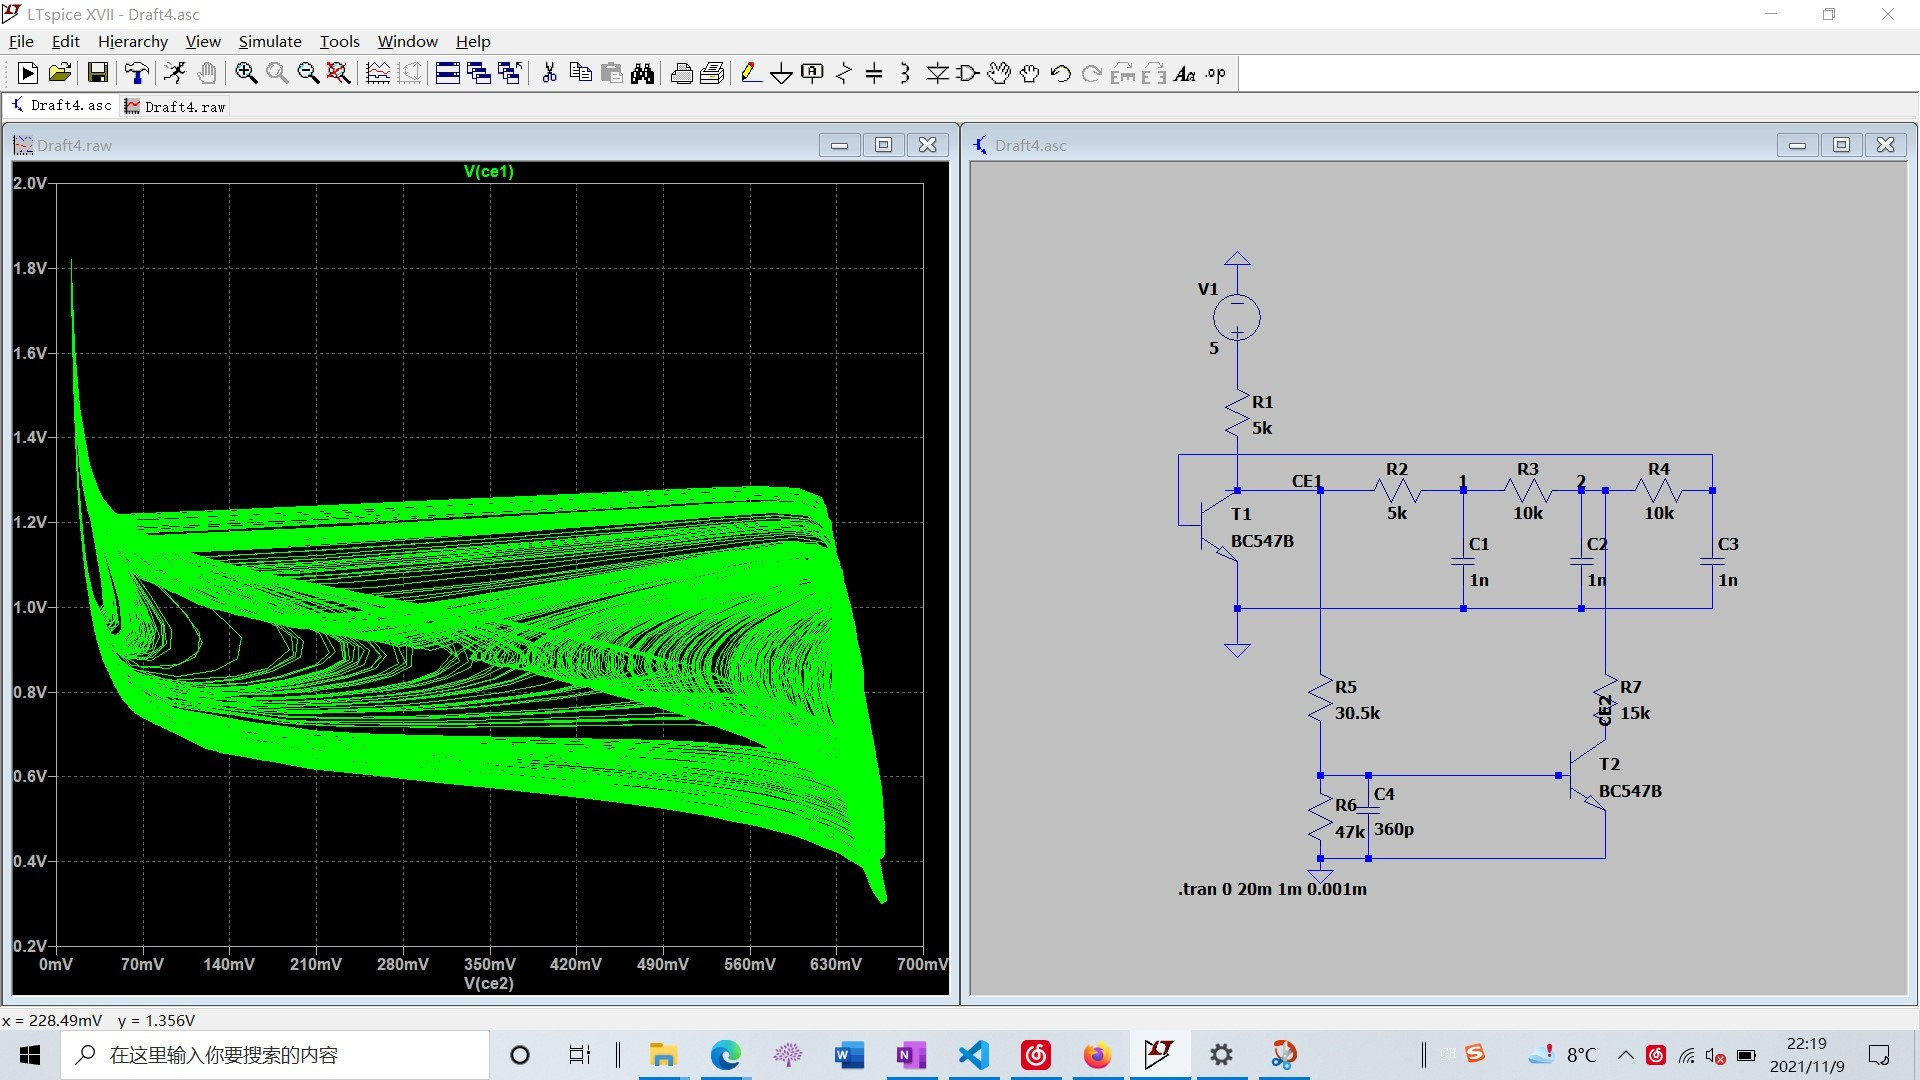
\includegraphics[width=2in]{1-3-30.5k-ce1ce2.jpg}
      \caption{$v_{CE1} - v_{CE2}$}
      \end{minipage}%
    }%
    \subfigure{
      \begin{minipage}[t]{0.33\linewidth}
      \centering
      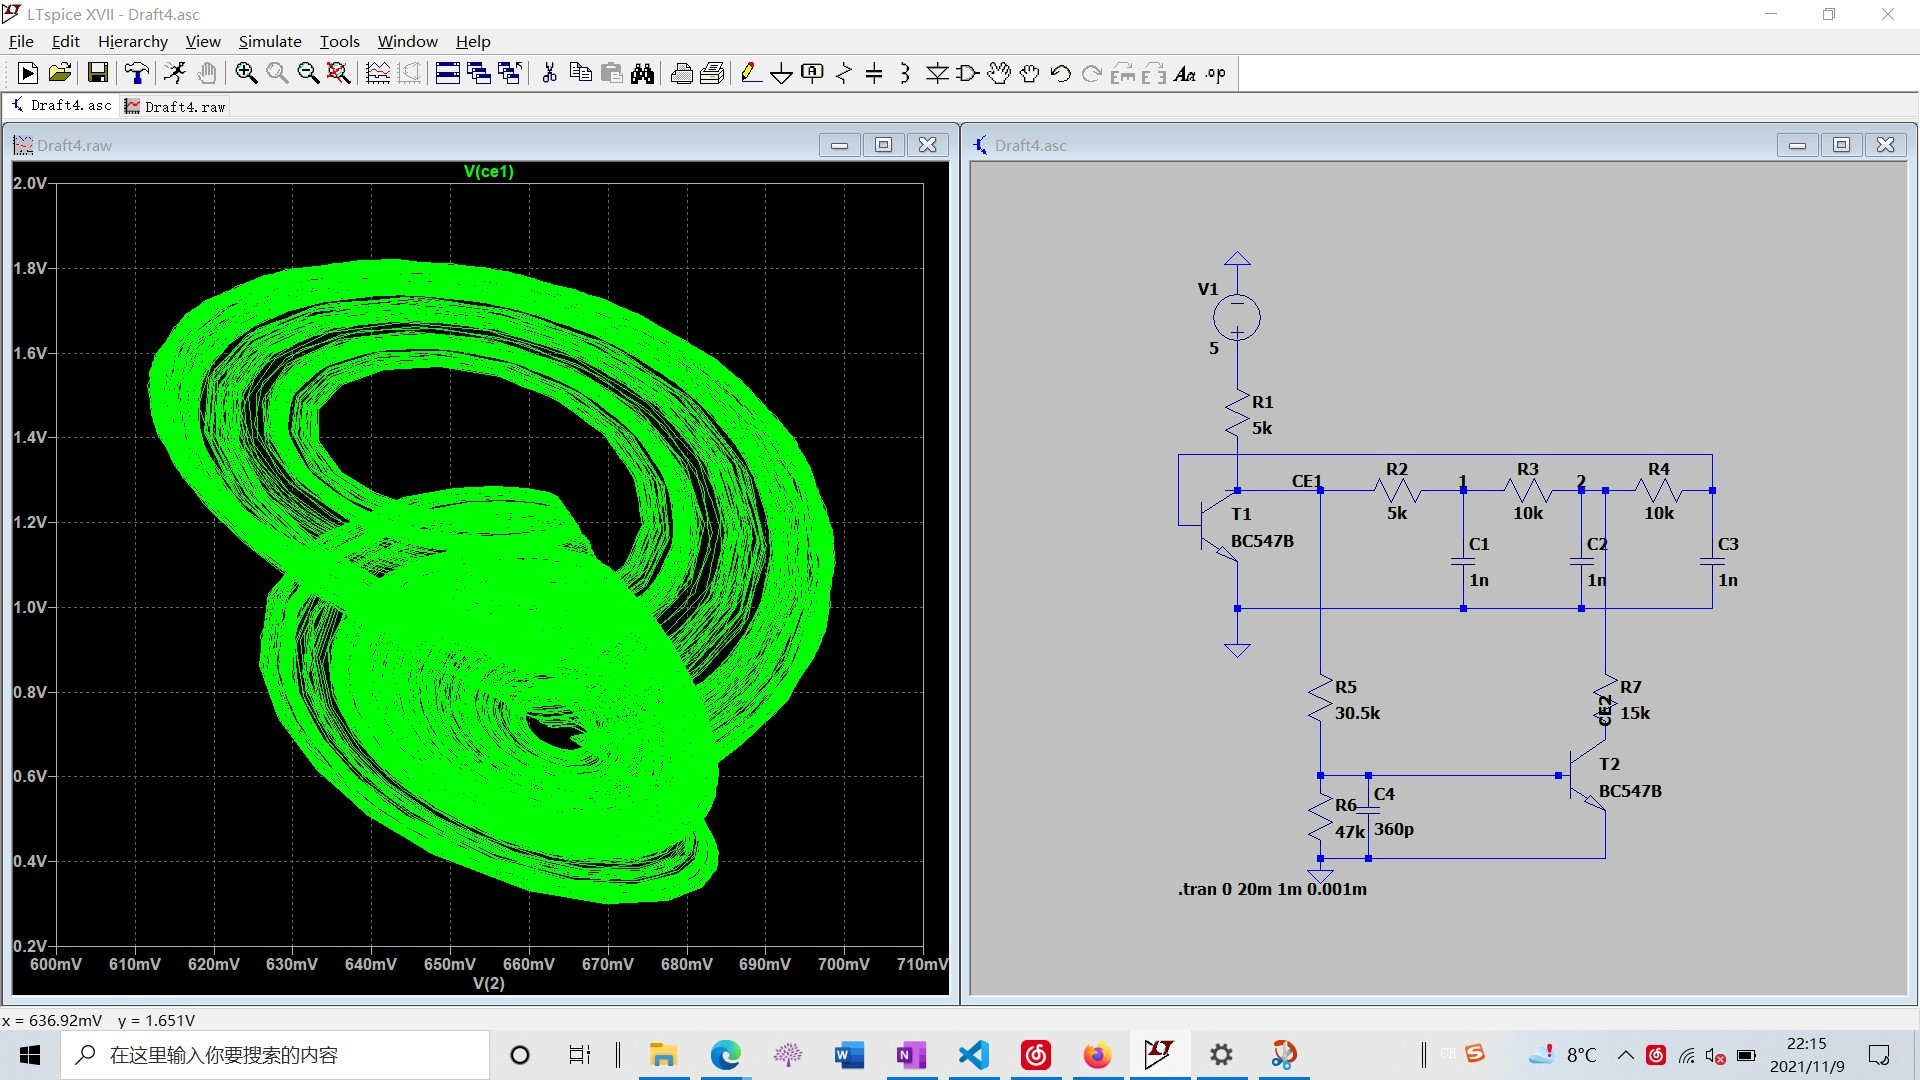
\includegraphics[width=2in]{1-3-30.5k-ce1-2.jpg}
      \caption{$v_{CE1} - v_{2}$}
      \end{minipage}%
    }%
    \subfigure{
      \begin{minipage}[t]{0.33\linewidth}
      \centering
      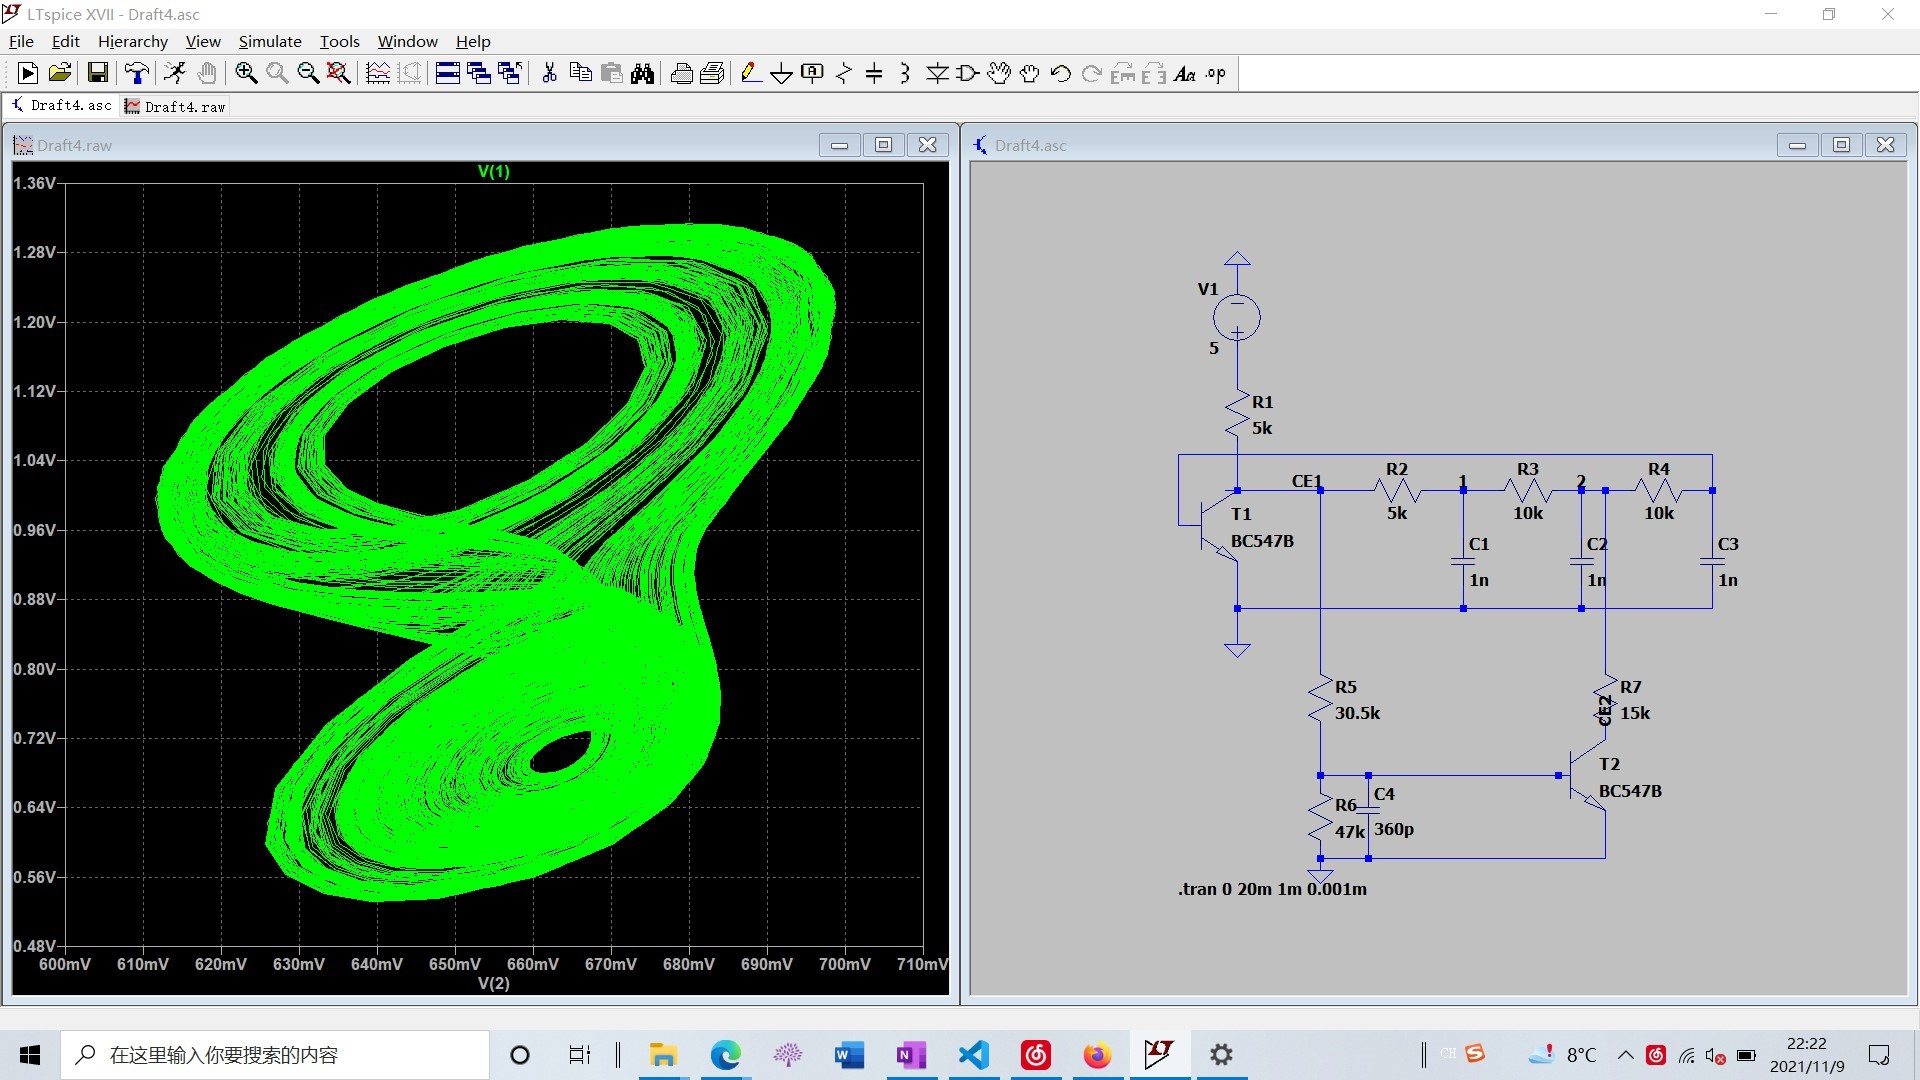
\includegraphics[width=2in]{1-3-30.5k-12.jpg}
      \caption{$v_{1} - v_{2}$}
      \end{minipage}%
    }%
  \end{figure}

 $R_5 = 31k \Omega$:

\begin{figure}[H]
  \centering
    \subfigure{
    \begin{minipage}[t]{0.33\linewidth}
    \centering
    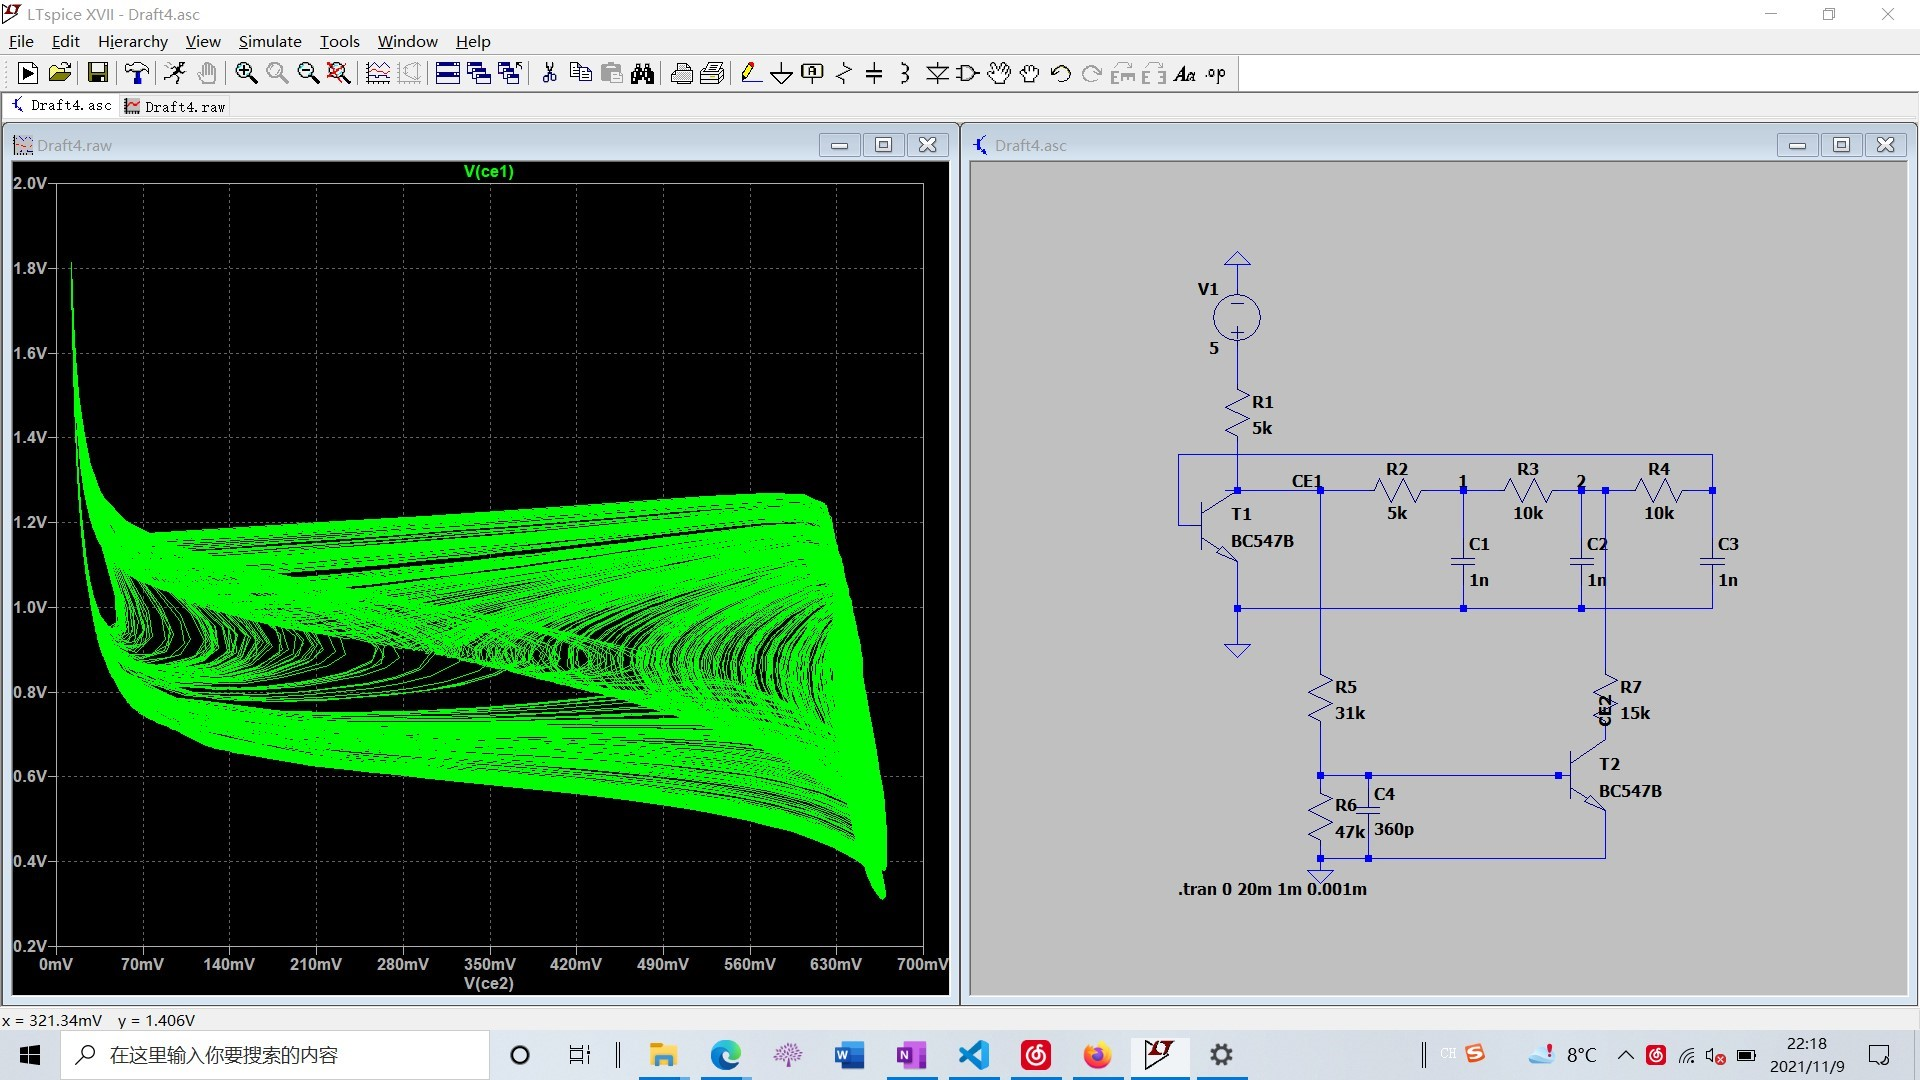
\includegraphics[width=2in]{1-3-31k-ce1ce2.jpg}
    \caption{$v_{CE1} - v_{CE2}$}
    \end{minipage}%
  }%
  \subfigure{
    \begin{minipage}[t]{0.33\linewidth}
    \centering
    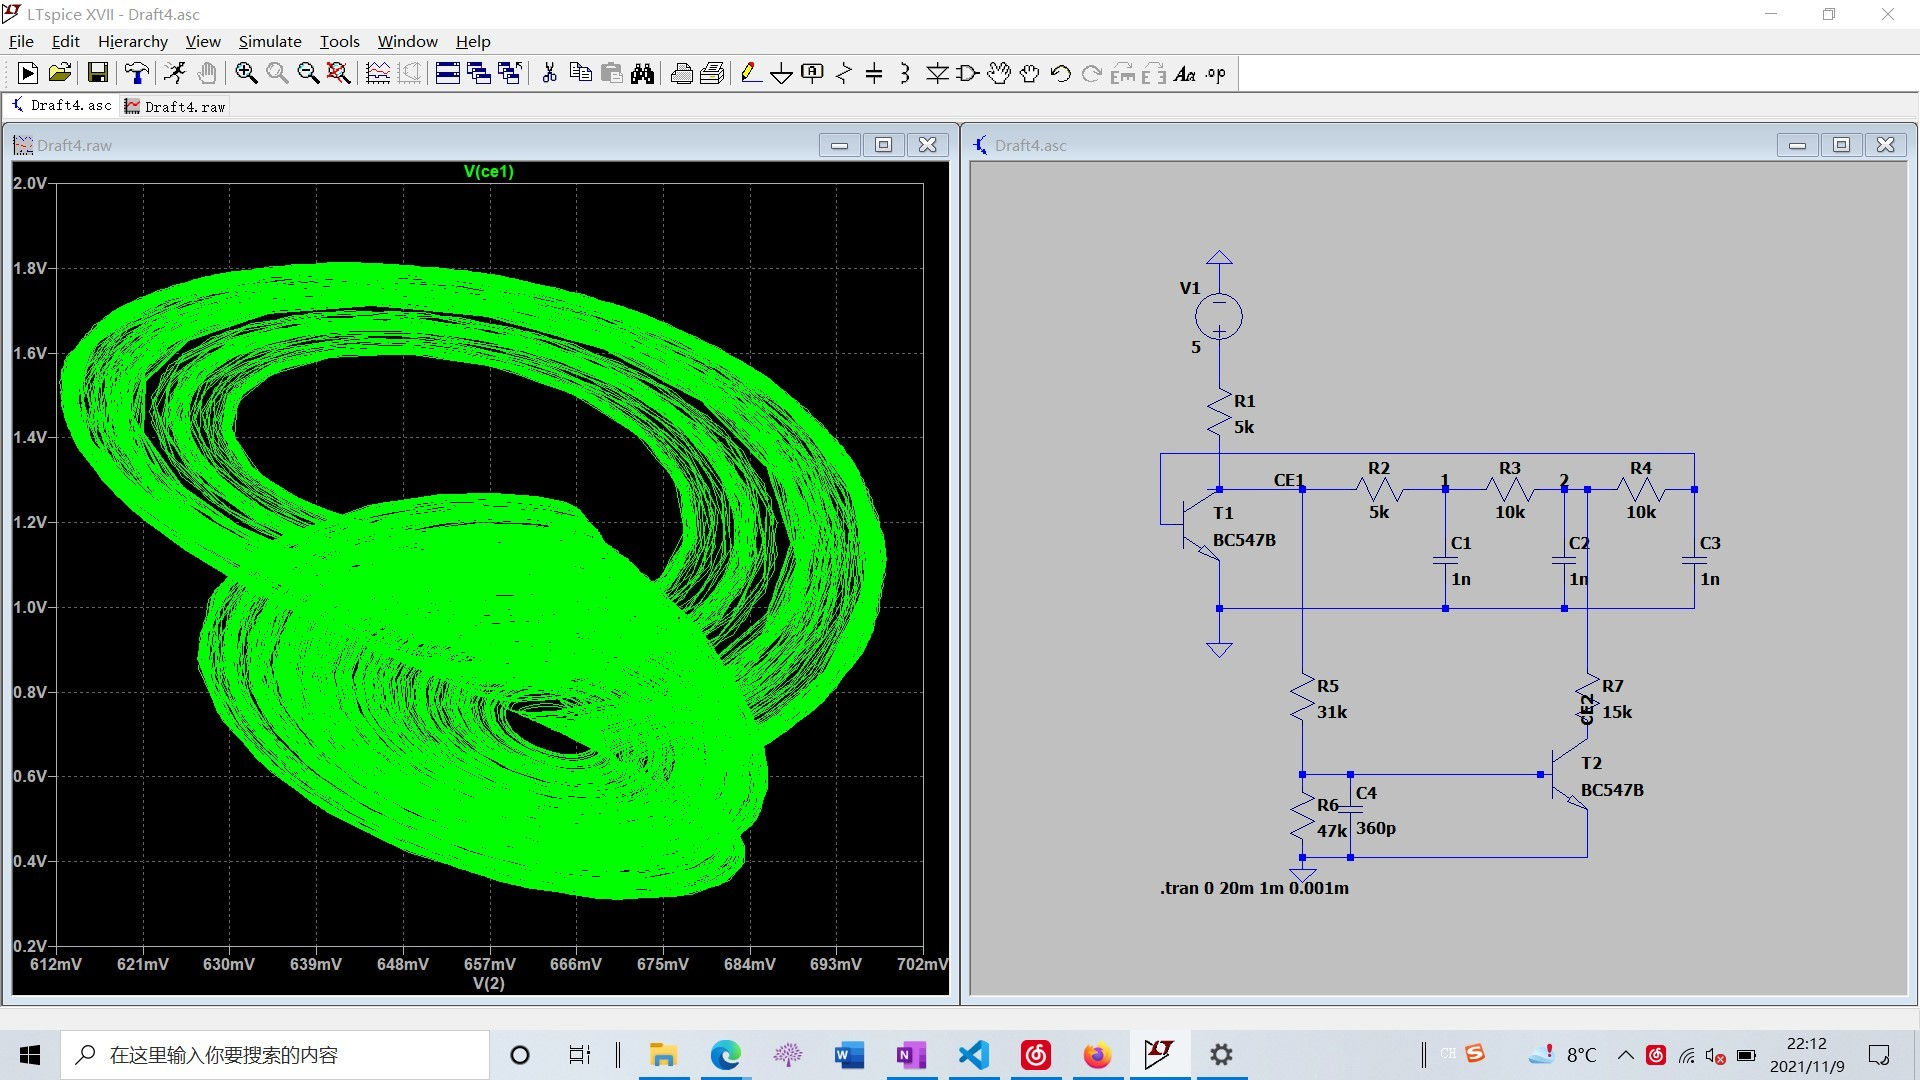
\includegraphics[width=2in]{1-3-31k-ce1-2.jpg}
    \caption{$v_{CE1} - v_{2}$}
    \end{minipage}%
  }%
  \subfigure{
    \begin{minipage}[t]{0.33\linewidth}
    \centering
    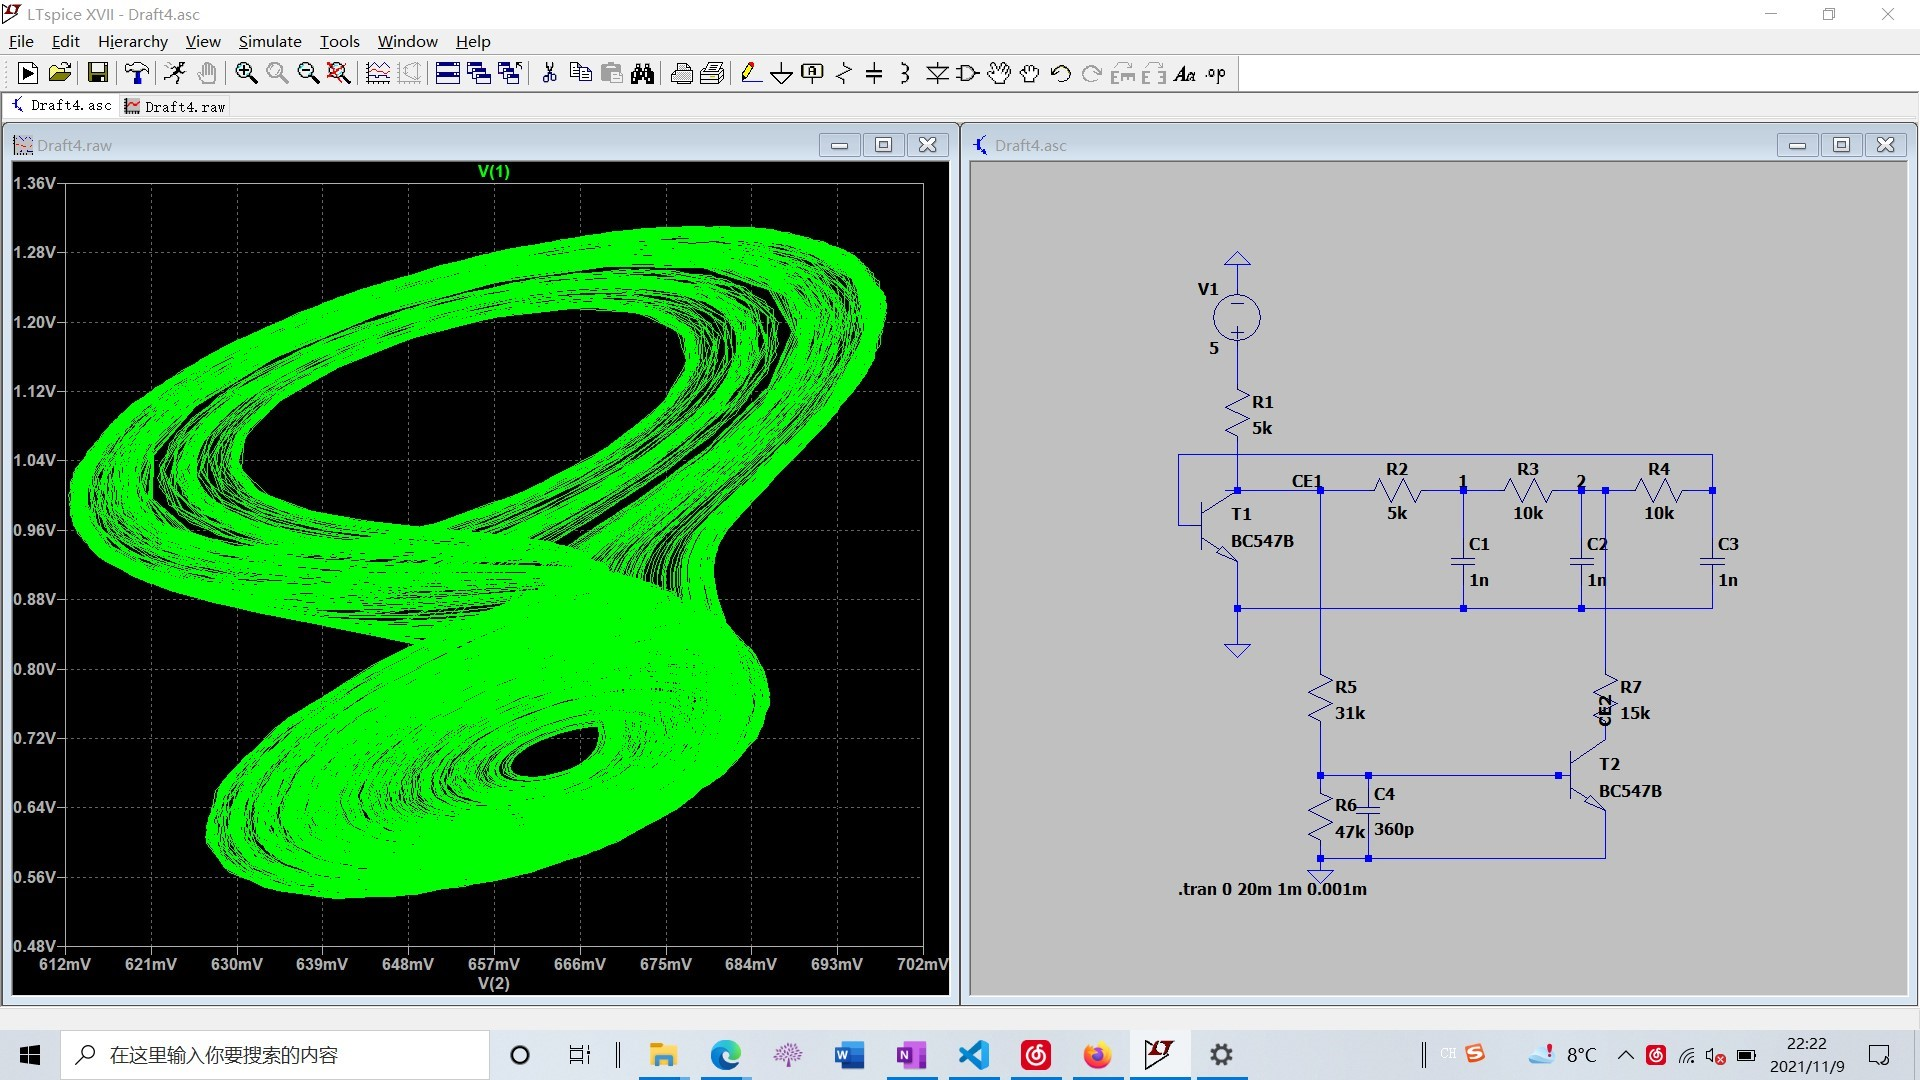
\includegraphics[width=2in]{1-3-31k-12.jpg}
    \caption{$v_{1} - v_{2}$}
    \end{minipage}%
  }%
\end{figure}
  $R_5 = 31.5k \Omega$:

  \begin{figure}[H]
    \centering
      \subfigure{
      \begin{minipage}[t]{0.33\linewidth}
      \centering
      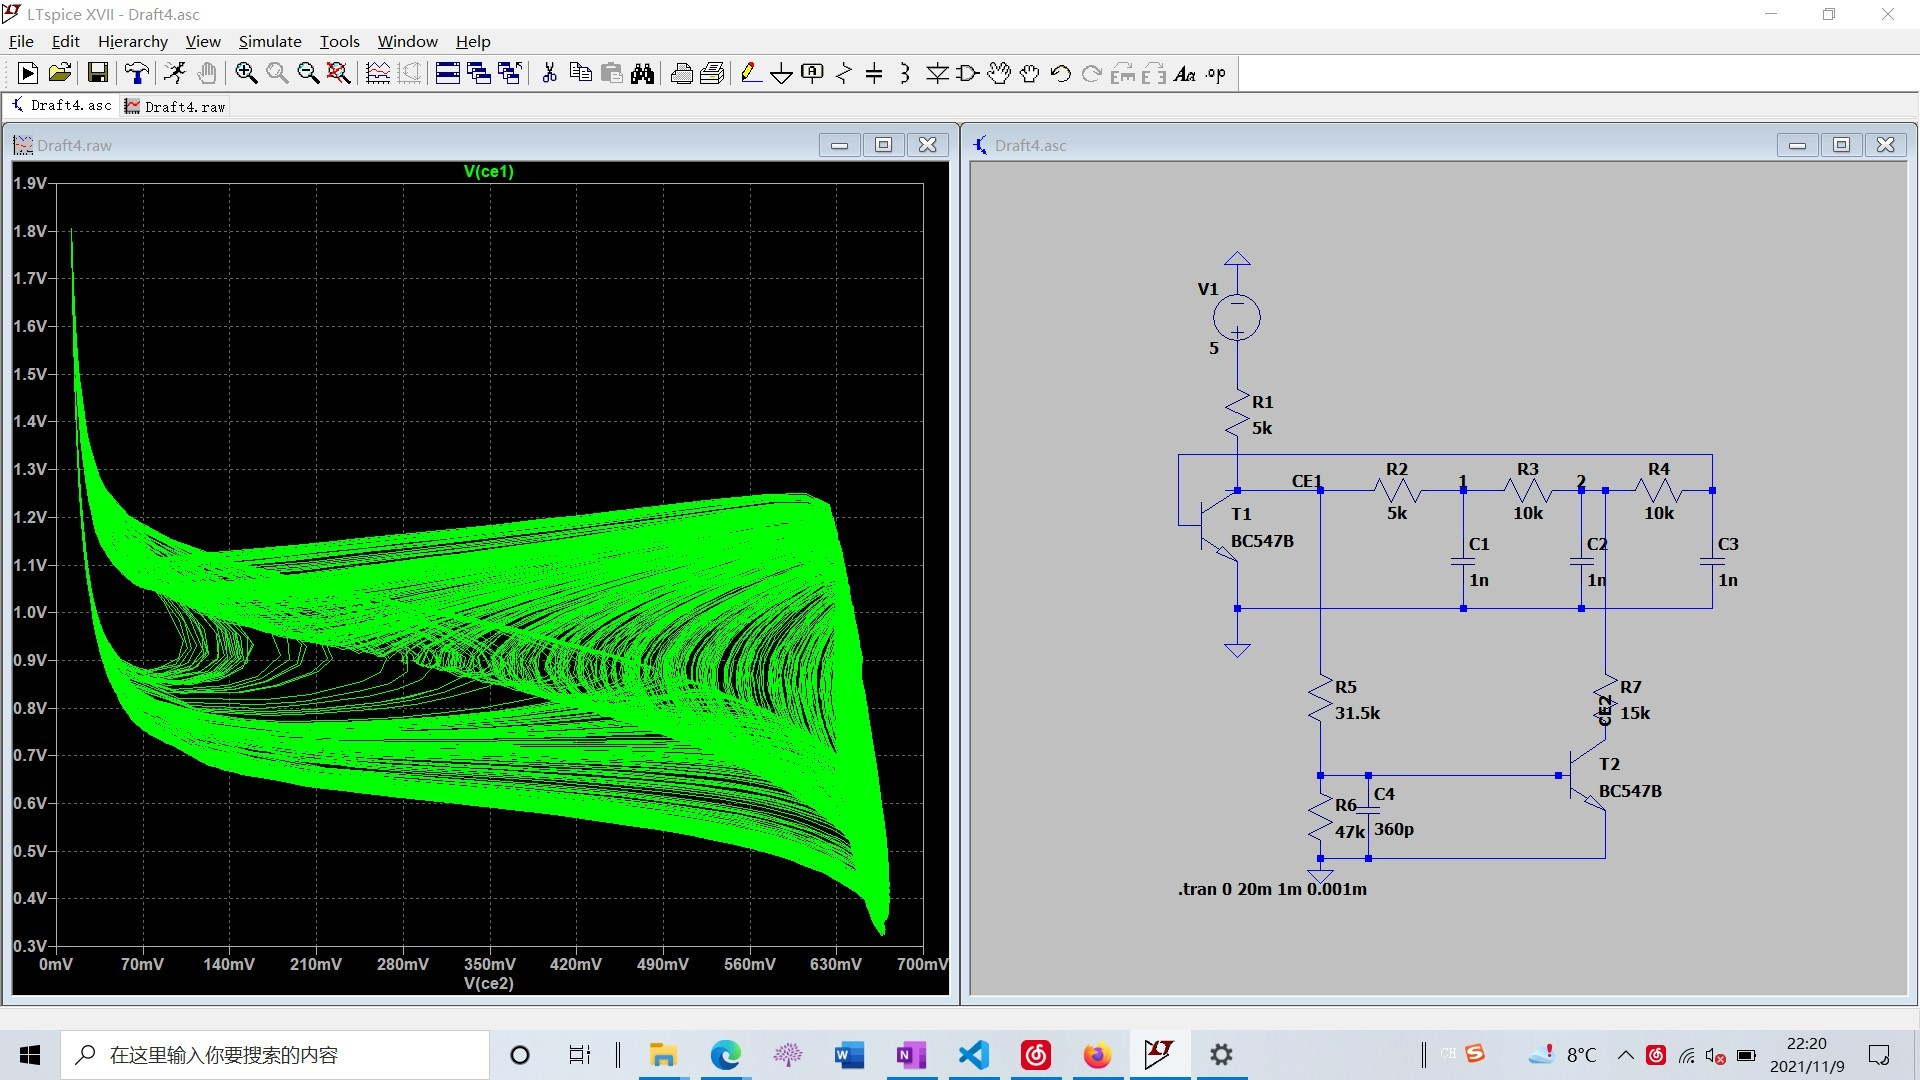
\includegraphics[width=2in]{1-3-31.5k-ce1ce2.jpg}
      \caption{$v_{CE1} - v_{CE2}$}
      \end{minipage}%
    }%
    \subfigure{
      \begin{minipage}[t]{0.33\linewidth}
      \centering
      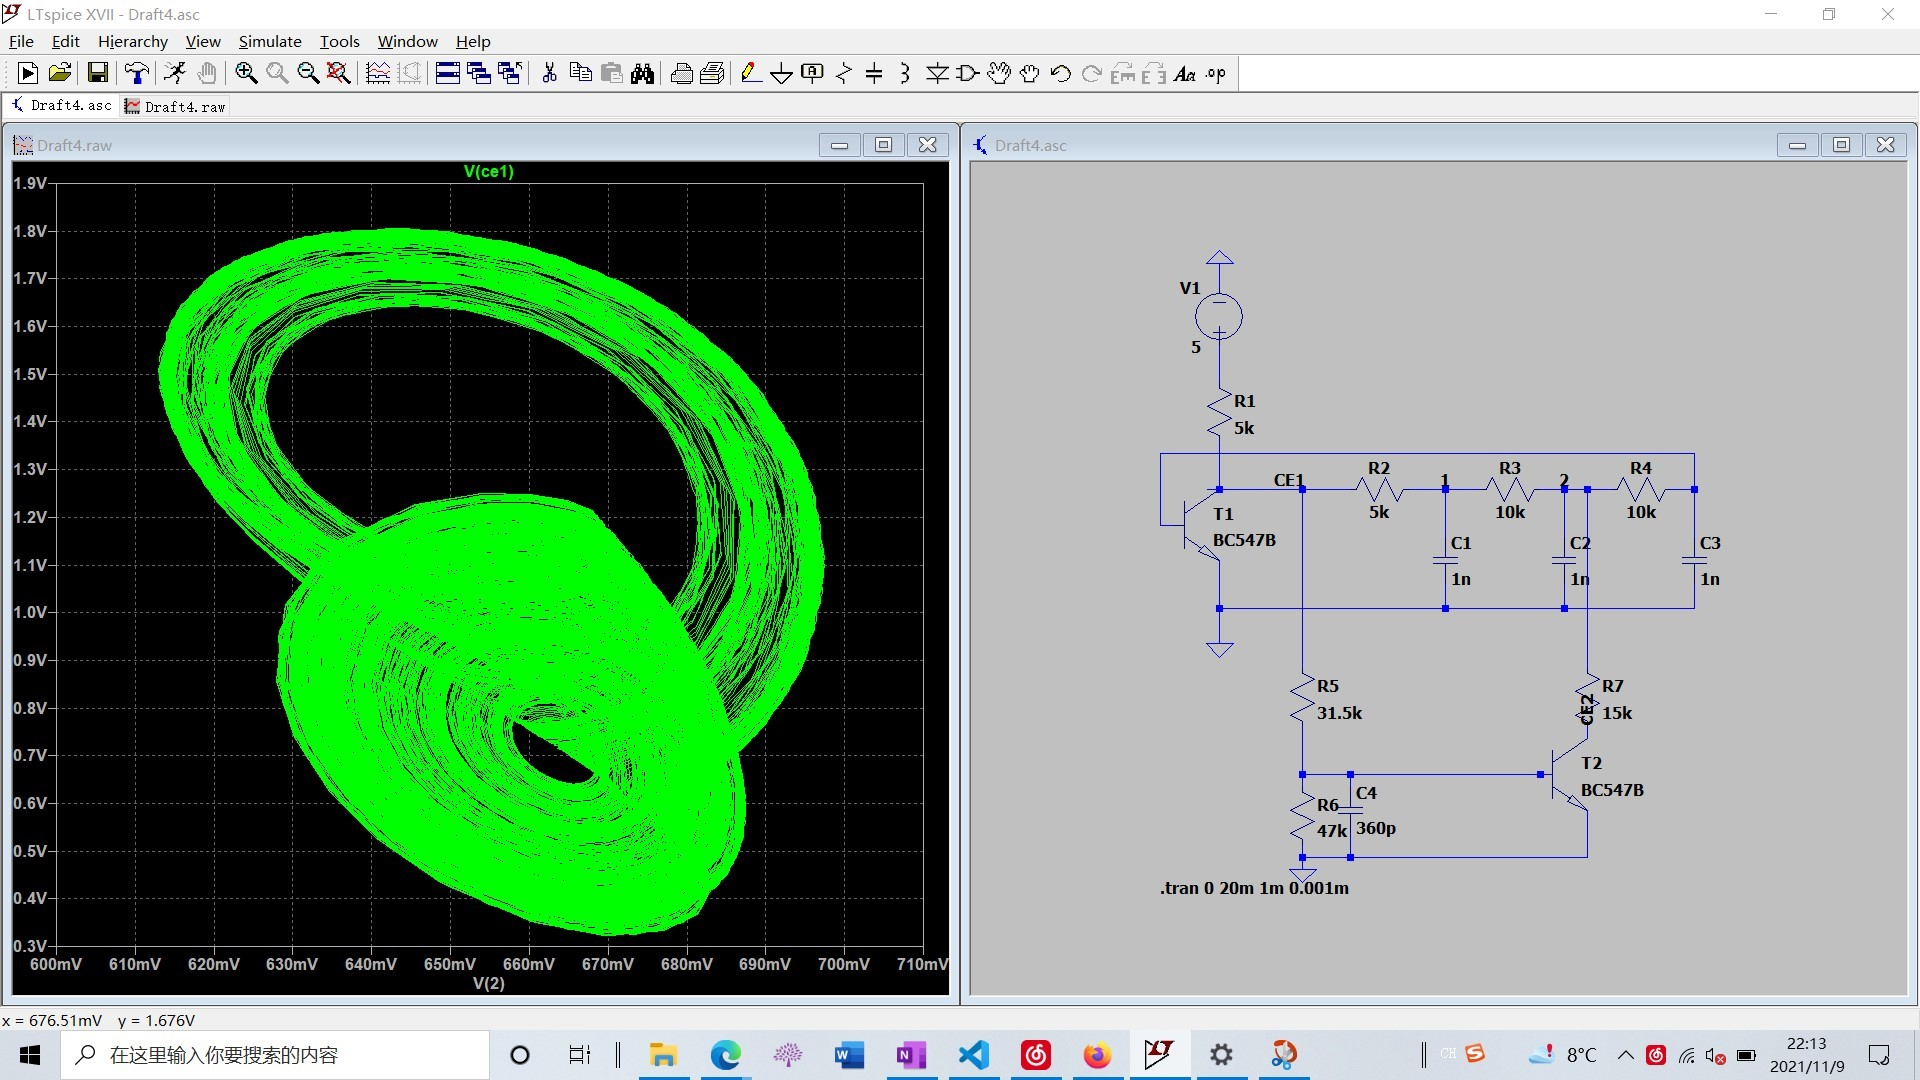
\includegraphics[width=2in]{1-3-31.5k-ce1-2.jpg}
      \caption{$v_{CE1} - v_{2}$}
      \end{minipage}%
    }%
    \subfigure{
      \begin{minipage}[t]{0.33\linewidth}
      \centering
      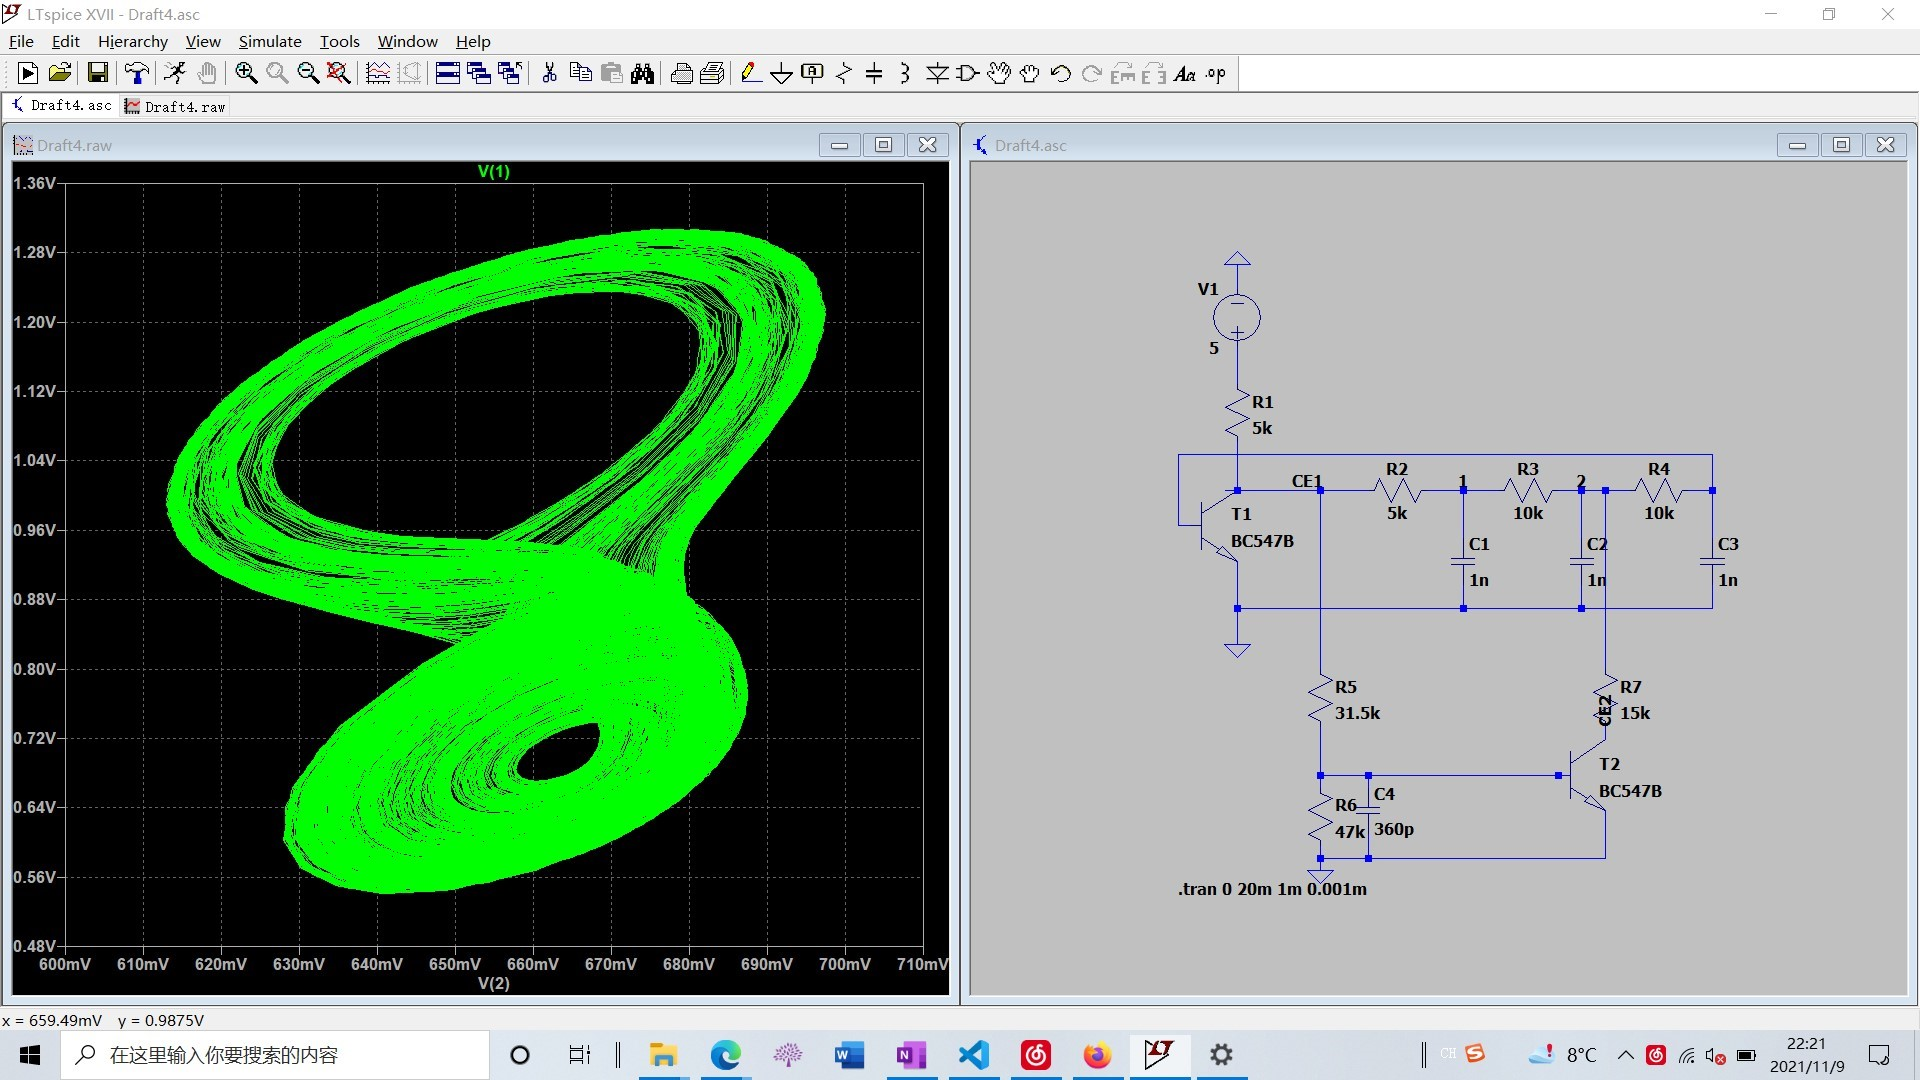
\includegraphics[width=2in]{1-3-31.5k-12.jpg}
      \caption{$v_{1} - v_{2}$}
      \end{minipage}%
    }%
  \end{figure}
    $R_5 = 32k \Omega$:

    \begin{figure}[H]
      \centering
        \subfigure{
        \begin{minipage}[t]{0.33\linewidth}
        \centering
        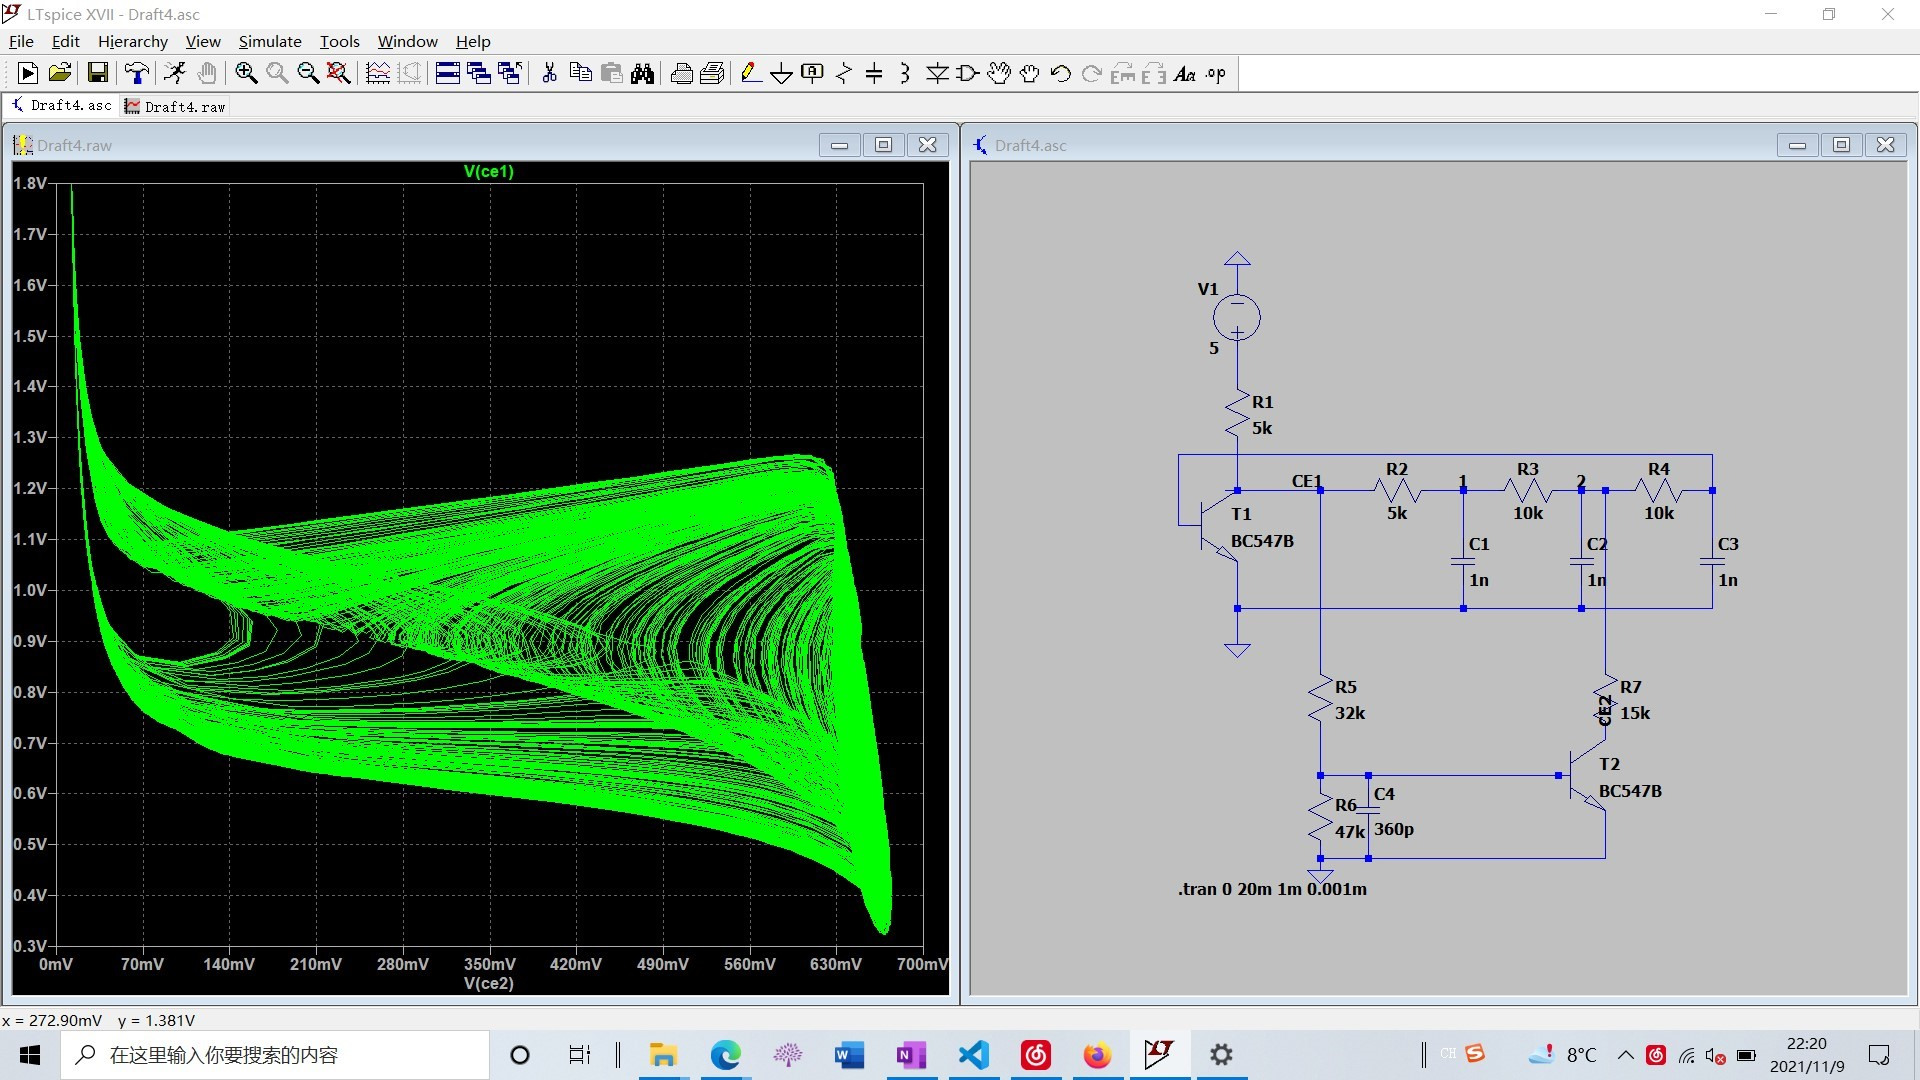
\includegraphics[width=2in]{1-3-32k-ce1ce2.jpg}
        \caption{$v_{CE1} - v_{CE2}$}
        \end{minipage}%
      }%
      \subfigure{
        \begin{minipage}[t]{0.33\linewidth}
        \centering
        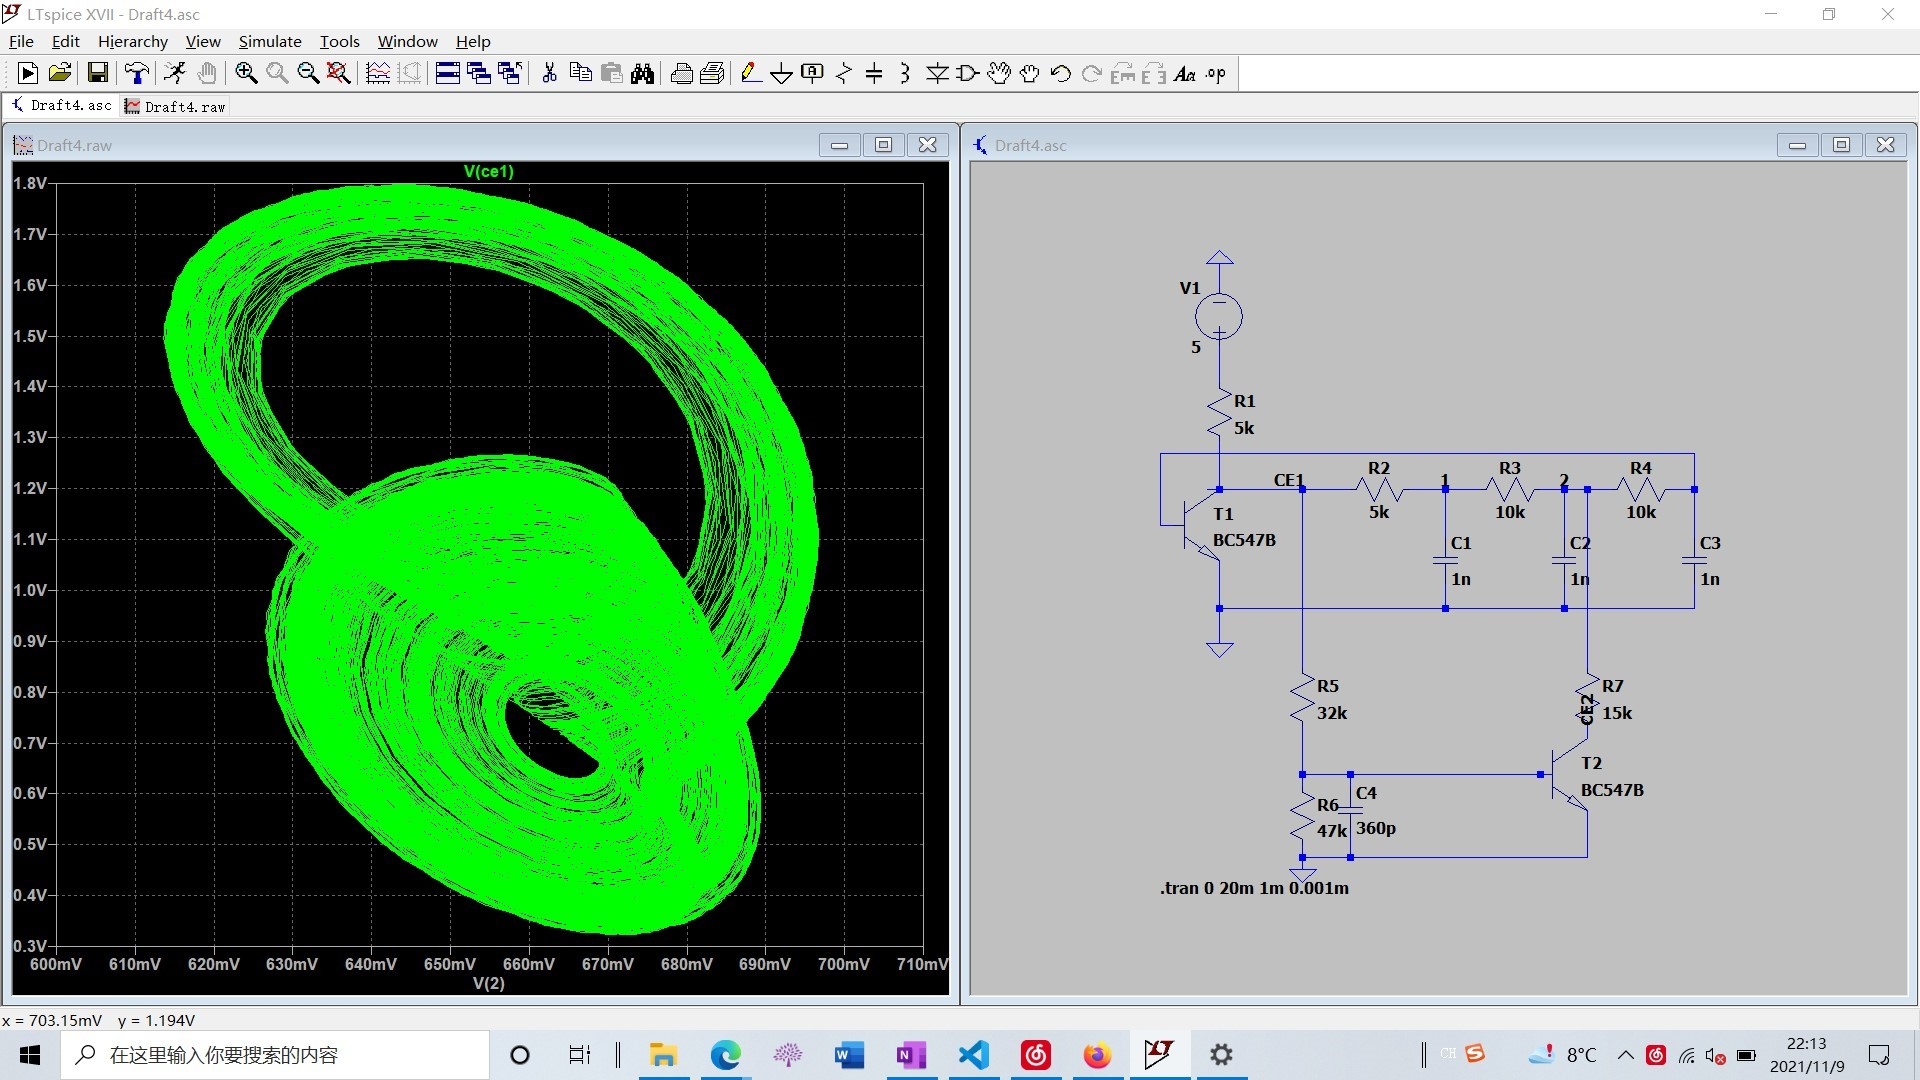
\includegraphics[width=2in]{1-3-32k-ce1-2.jpg}
        \caption{$v_{CE1} - v_{2}$}
        \end{minipage}%
      }%
      \subfigure{
        \begin{minipage}[t]{0.33\linewidth}
        \centering
        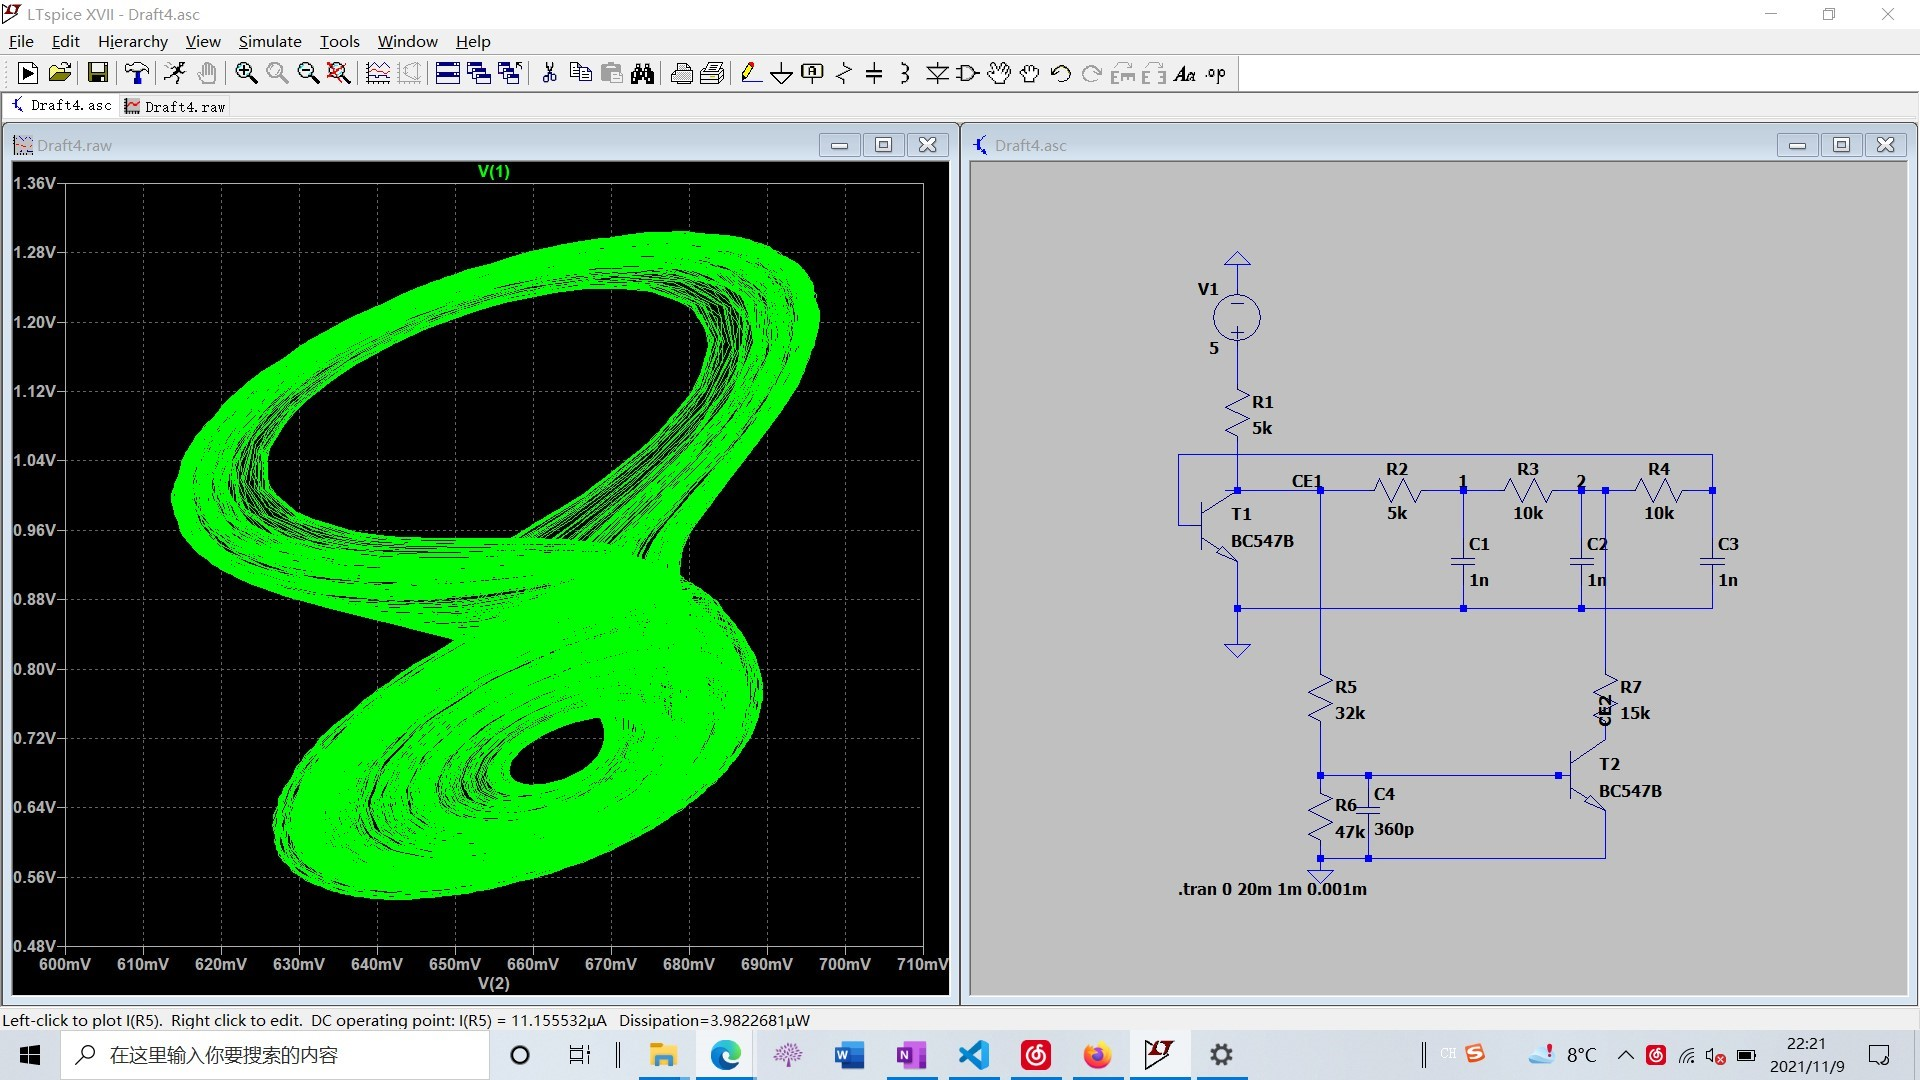
\includegraphics[width=2in]{1-3-32k-12.jpg}
        \caption{$v_{1} - v_{2}$}
        \end{minipage}%
      }%
  
\end{figure}


%%%%%%%%%%%%%%%%%%%%%%%%%%%%%%%%%%%%%%%%%%%%%%%%%%%%%%%%%
%%%%%%%%%%%%%%%%%%%%%%%%%%%%%%%%%%%%%%%%%%%%%%%%%%%%%%%%%%


$R_5 = 30k \Omega$:

\begin{figure}[H]
  \centering
    \subfigure{
    \begin{minipage}[t]{0.33\linewidth}
    \centering
    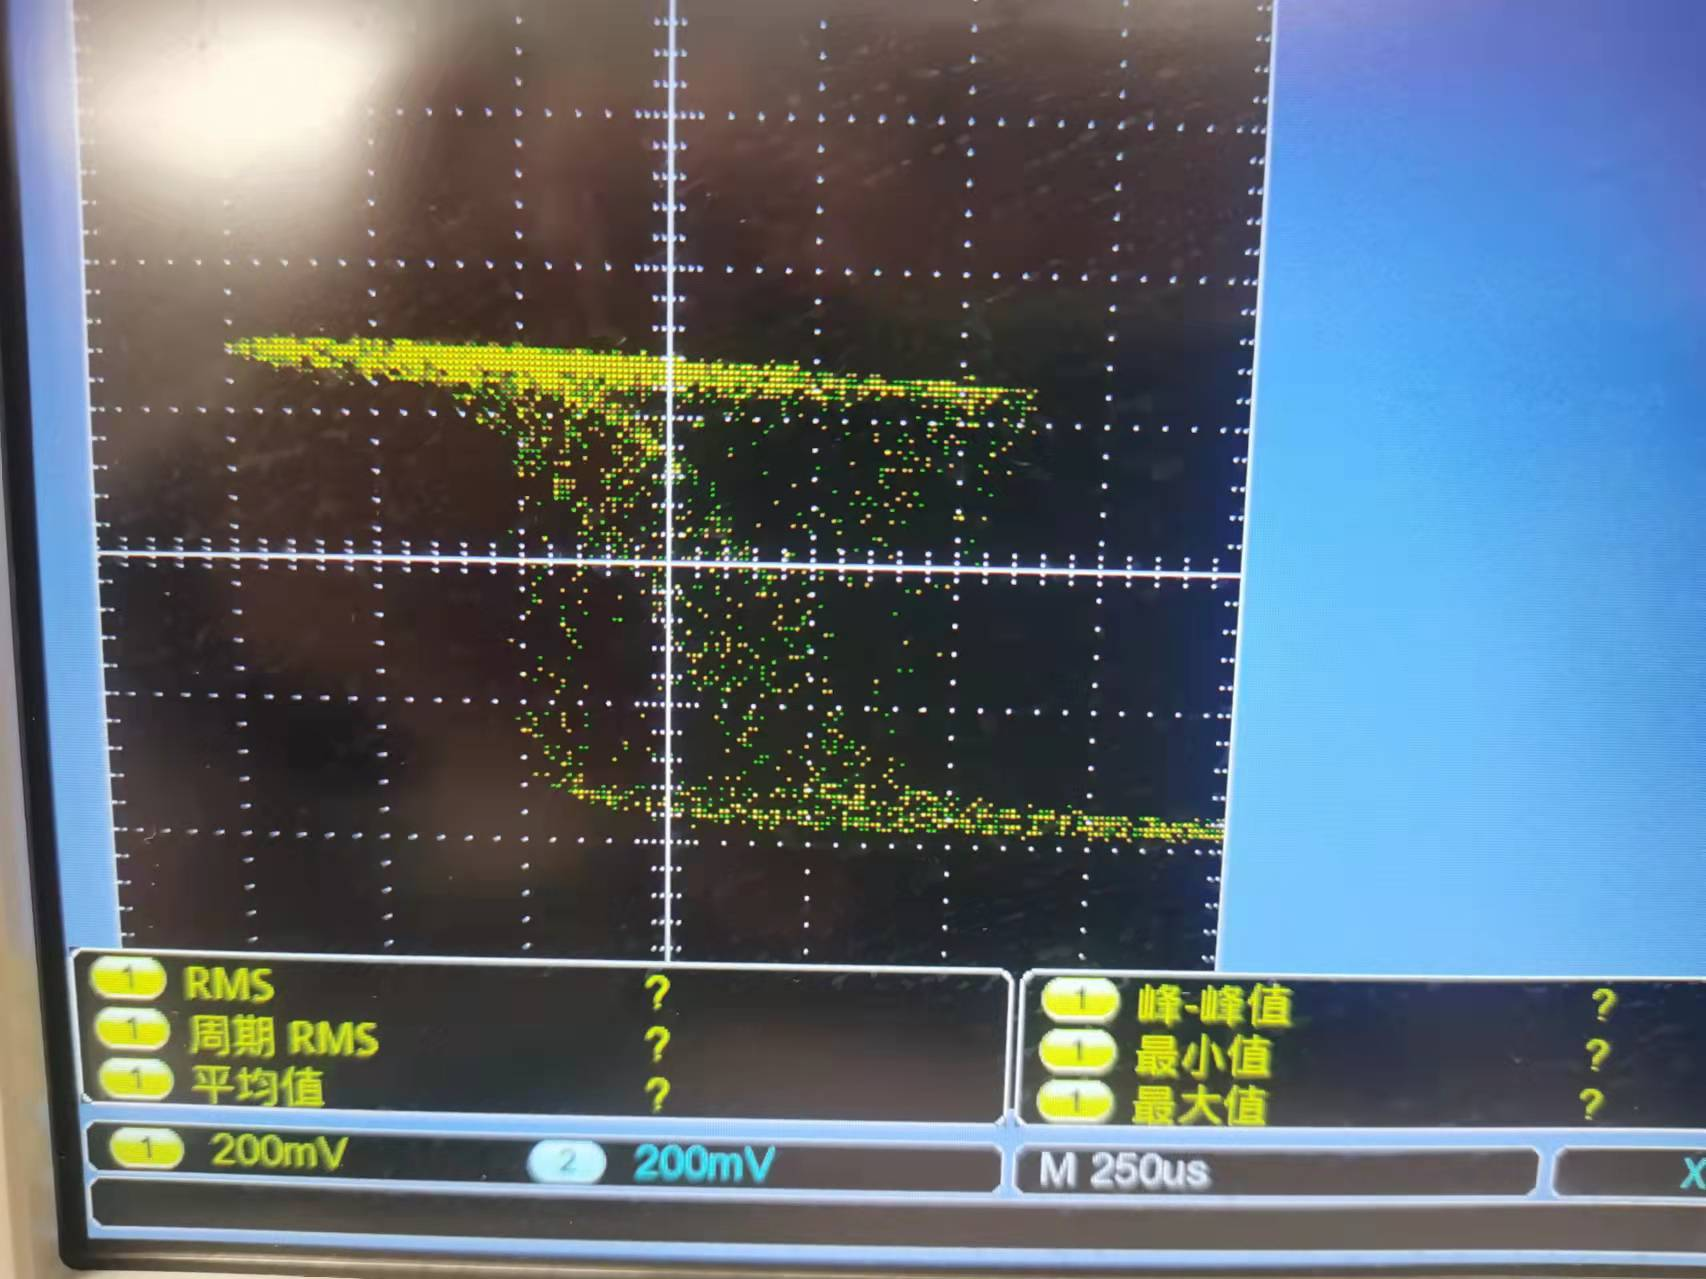
\includegraphics[width=2in]{1-3-30k-ce1ce2-r.jpg}
    \caption{$v_{CE1} - v_{CE2}$}
    \end{minipage}%
  }%
  \subfigure{
    \begin{minipage}[t]{0.33\linewidth}
    \centering
    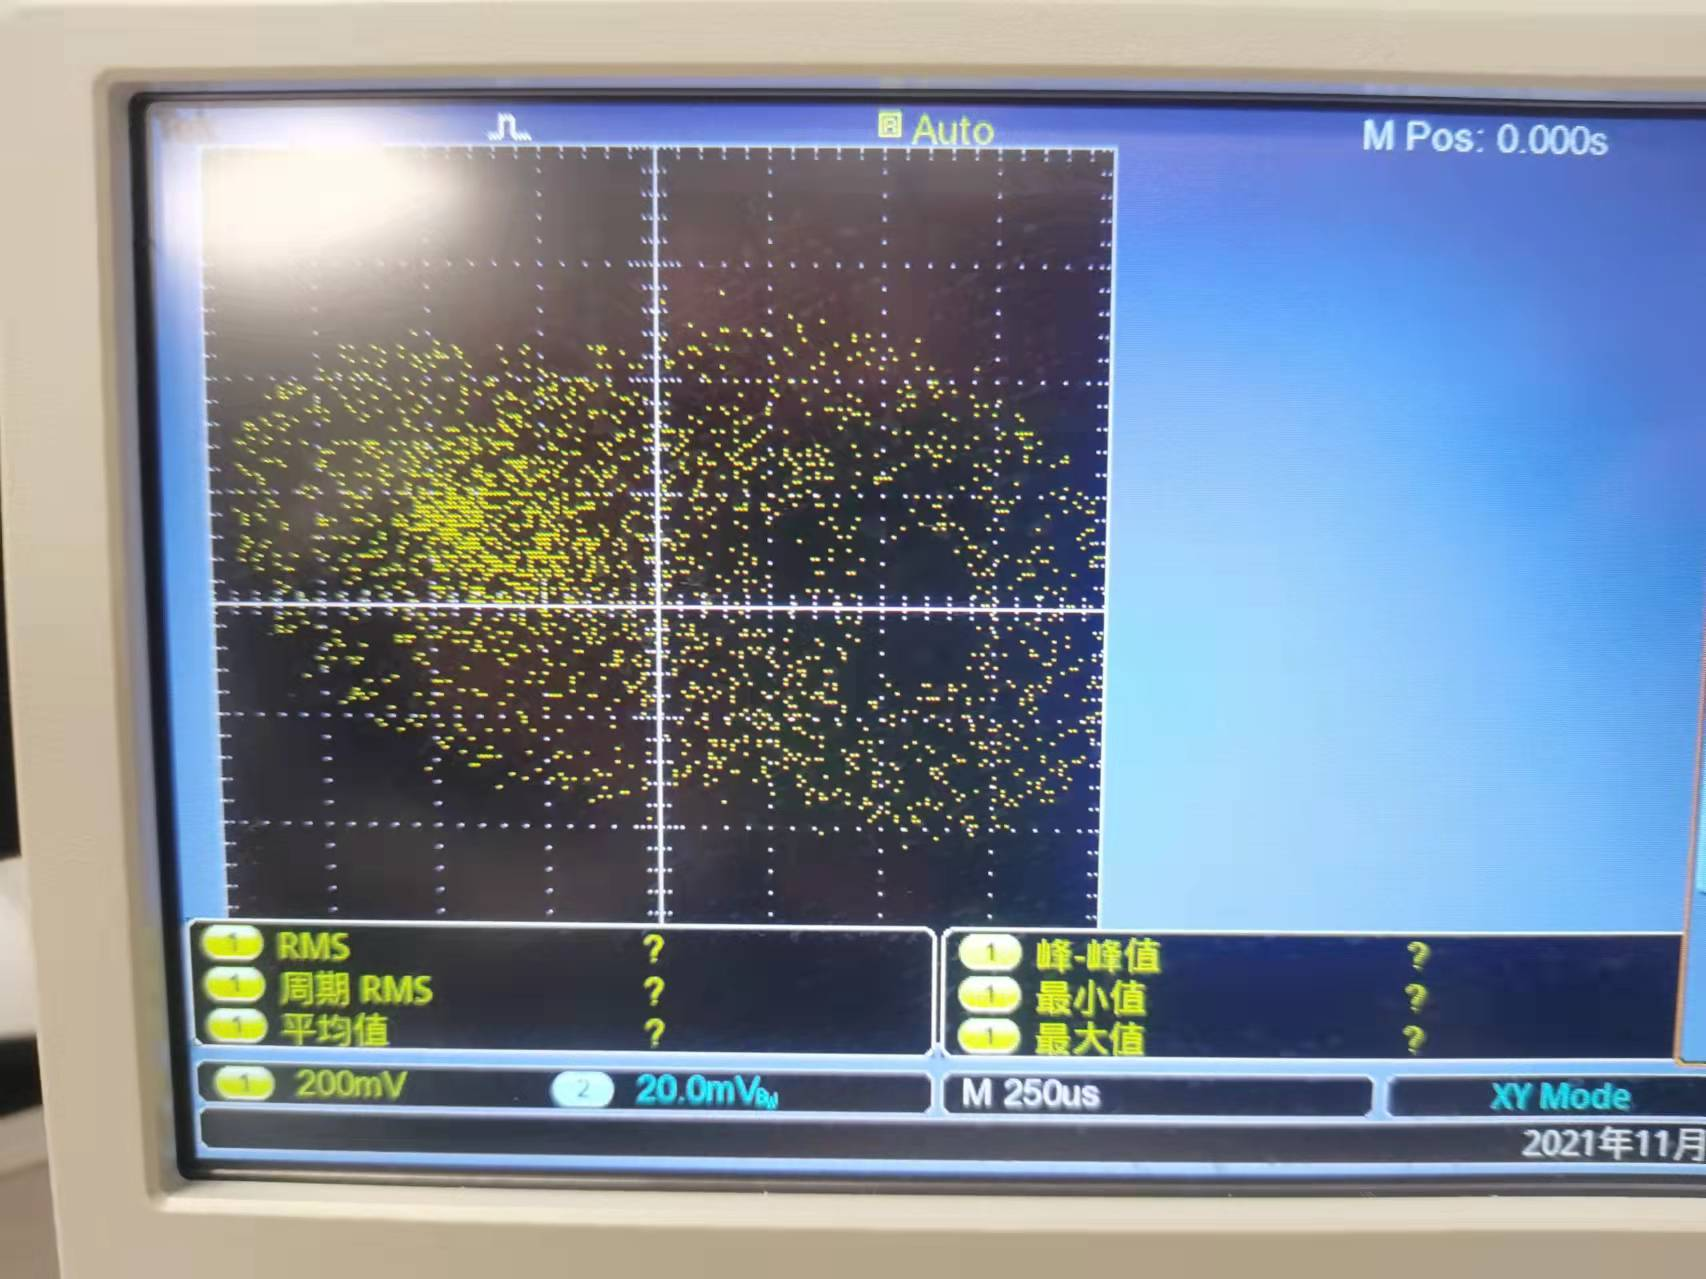
\includegraphics[width=2in]{1-3-30k-ce1-2-r.jpg}
    \caption{$v_{CE1} - v_{2}$}
    \end{minipage}%
  }%
  \subfigure{
    \begin{minipage}[t]{0.33\linewidth}
    \centering
    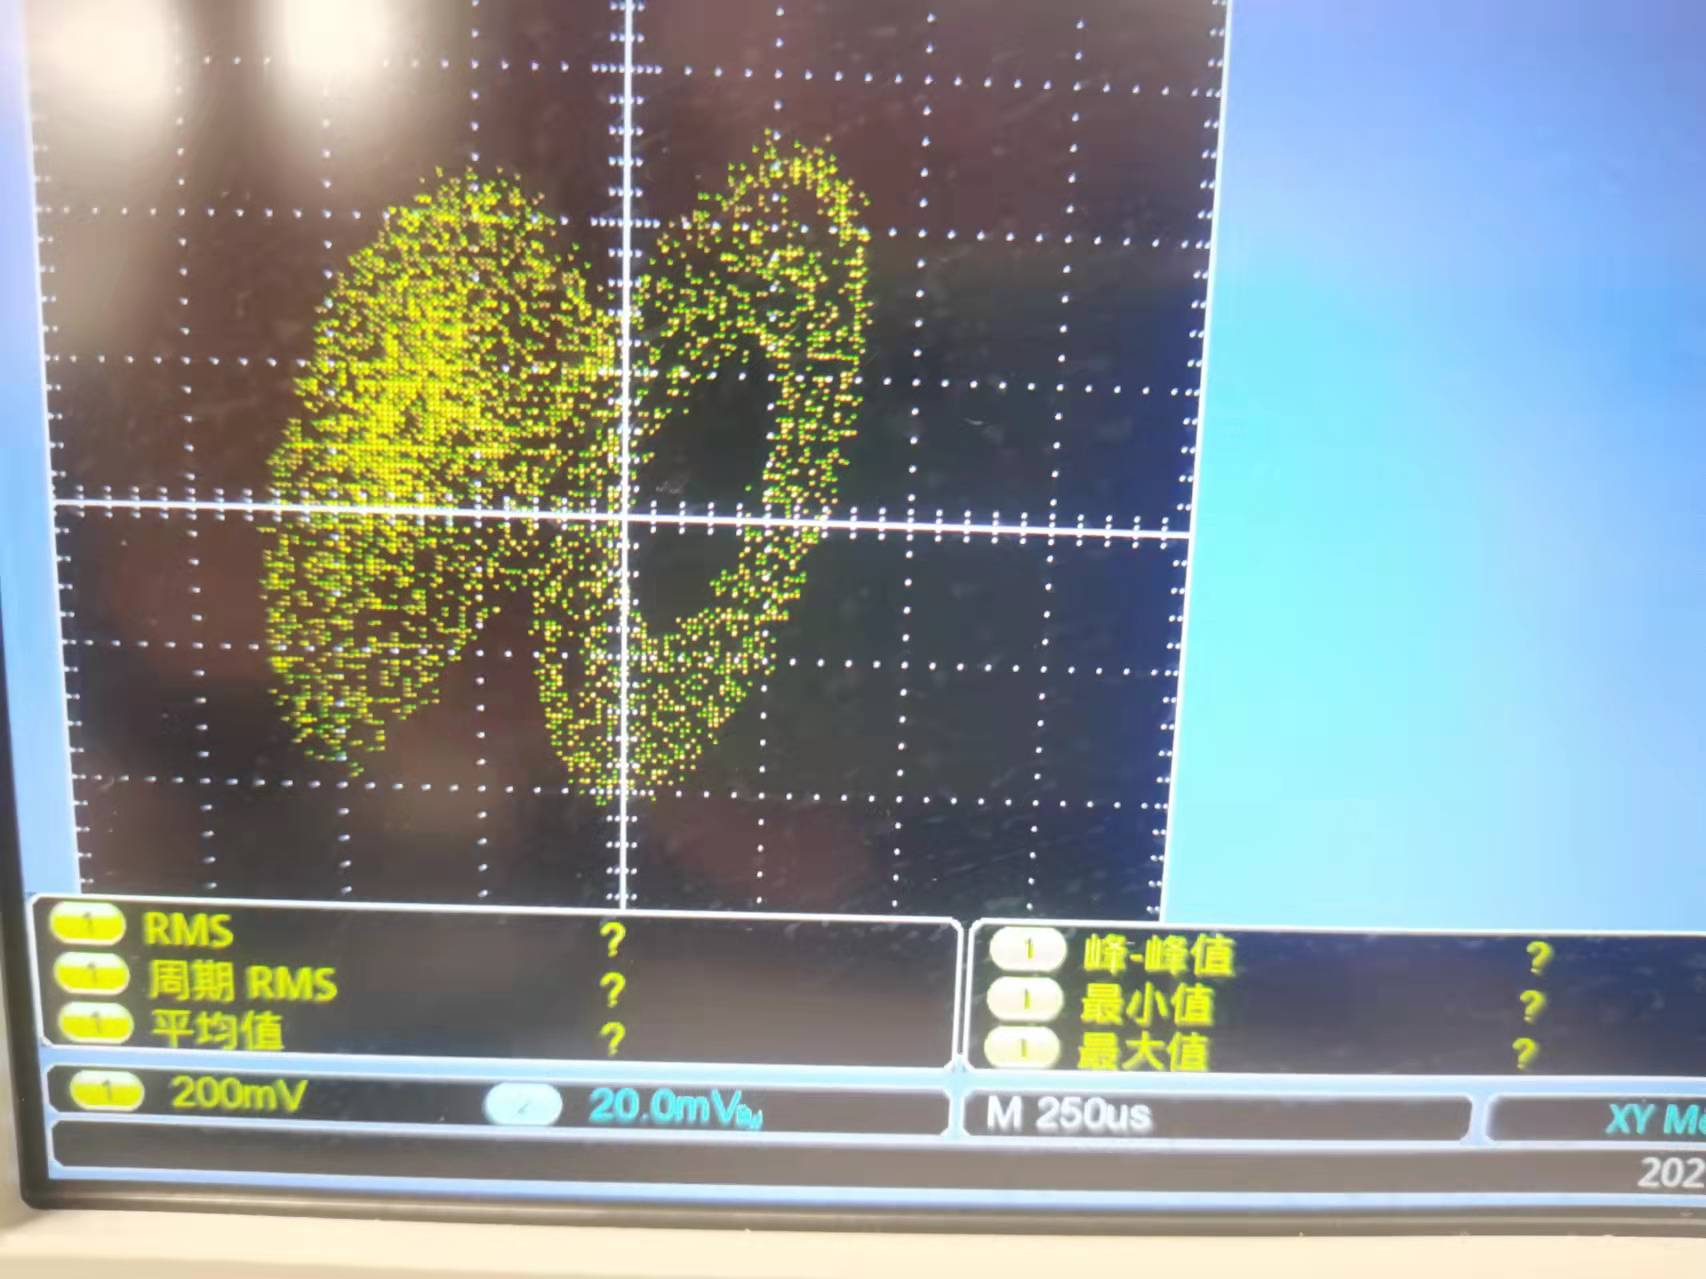
\includegraphics[width=2in]{1-3-30k-1-2-r.jpg}
    \caption{$v_{1} - v_{2}$}
    \end{minipage}%
  }%
  \end{figure}

  $R_5 = 30.5k \Omega$:

  \begin{figure}[H]
    \centering
      \subfigure{
      \begin{minipage}[t]{0.33\linewidth}
      \centering
      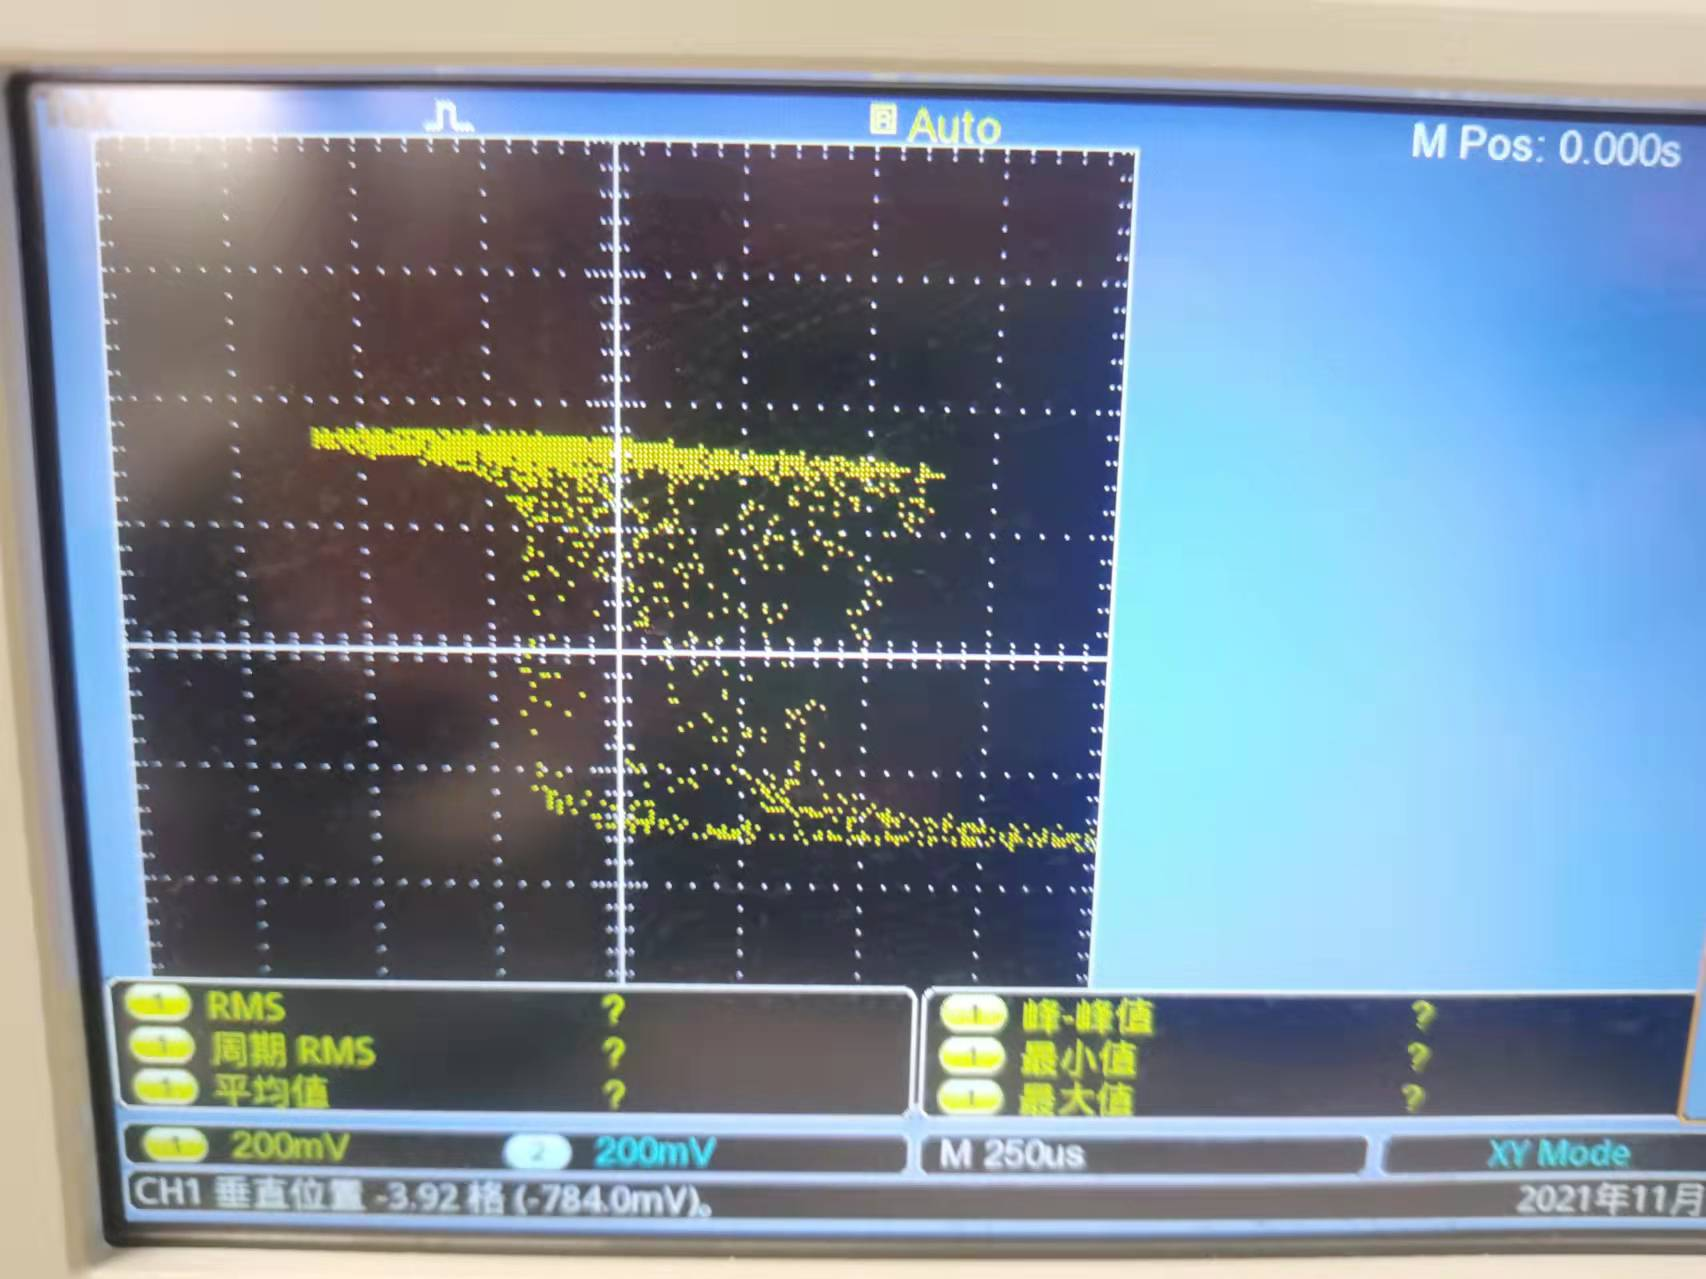
\includegraphics[width=2in]{1-3-30.5k-ce1ce2-r.jpg}
      \caption{$v_{CE1} - v_{CE2}$}
      \end{minipage}%
    }%
    \subfigure{
      \begin{minipage}[t]{0.33\linewidth}
      \centering
      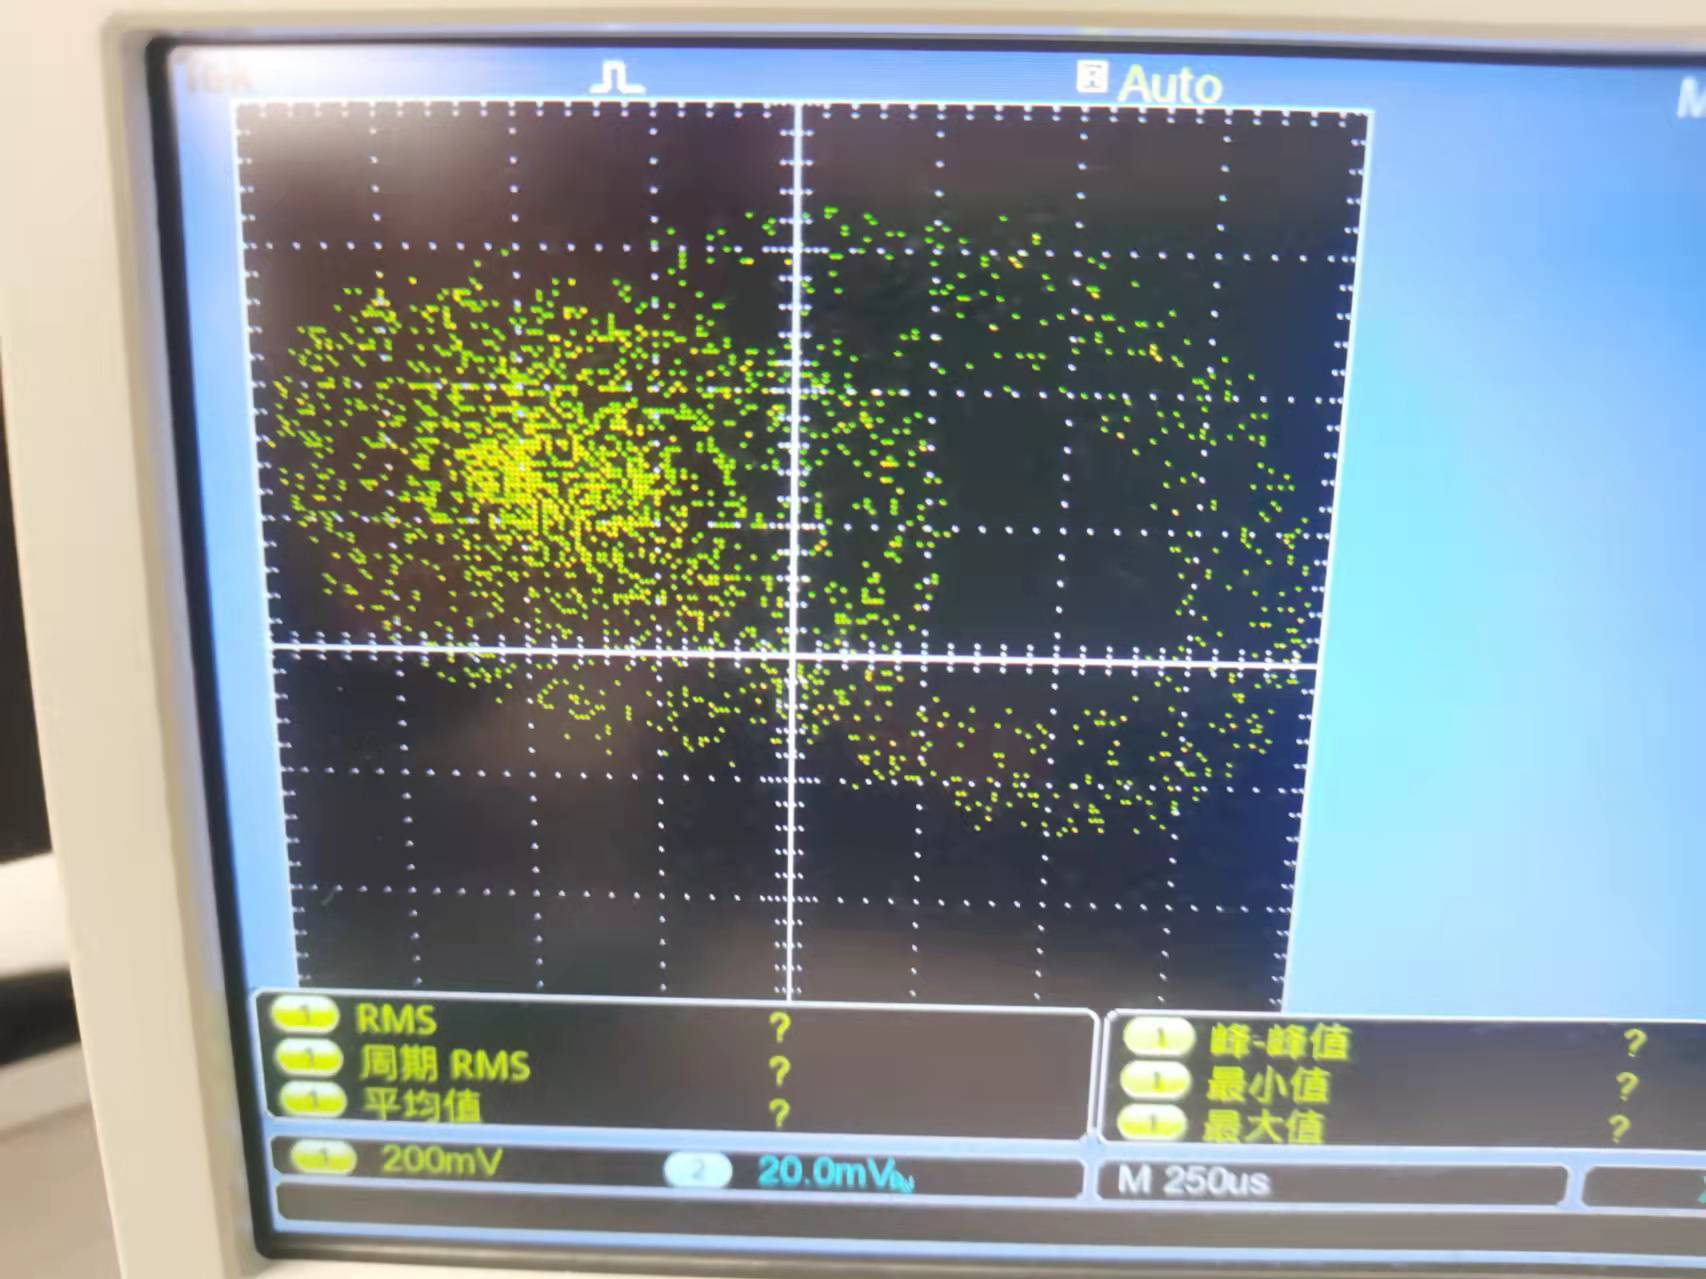
\includegraphics[width=2in]{1-3-30.5k-ce1-2-r.jpg}
      \caption{$v_{CE1} - v_{2}$}
      \end{minipage}%
    }%
    \subfigure{
      \begin{minipage}[t]{0.33\linewidth}
      \centering
      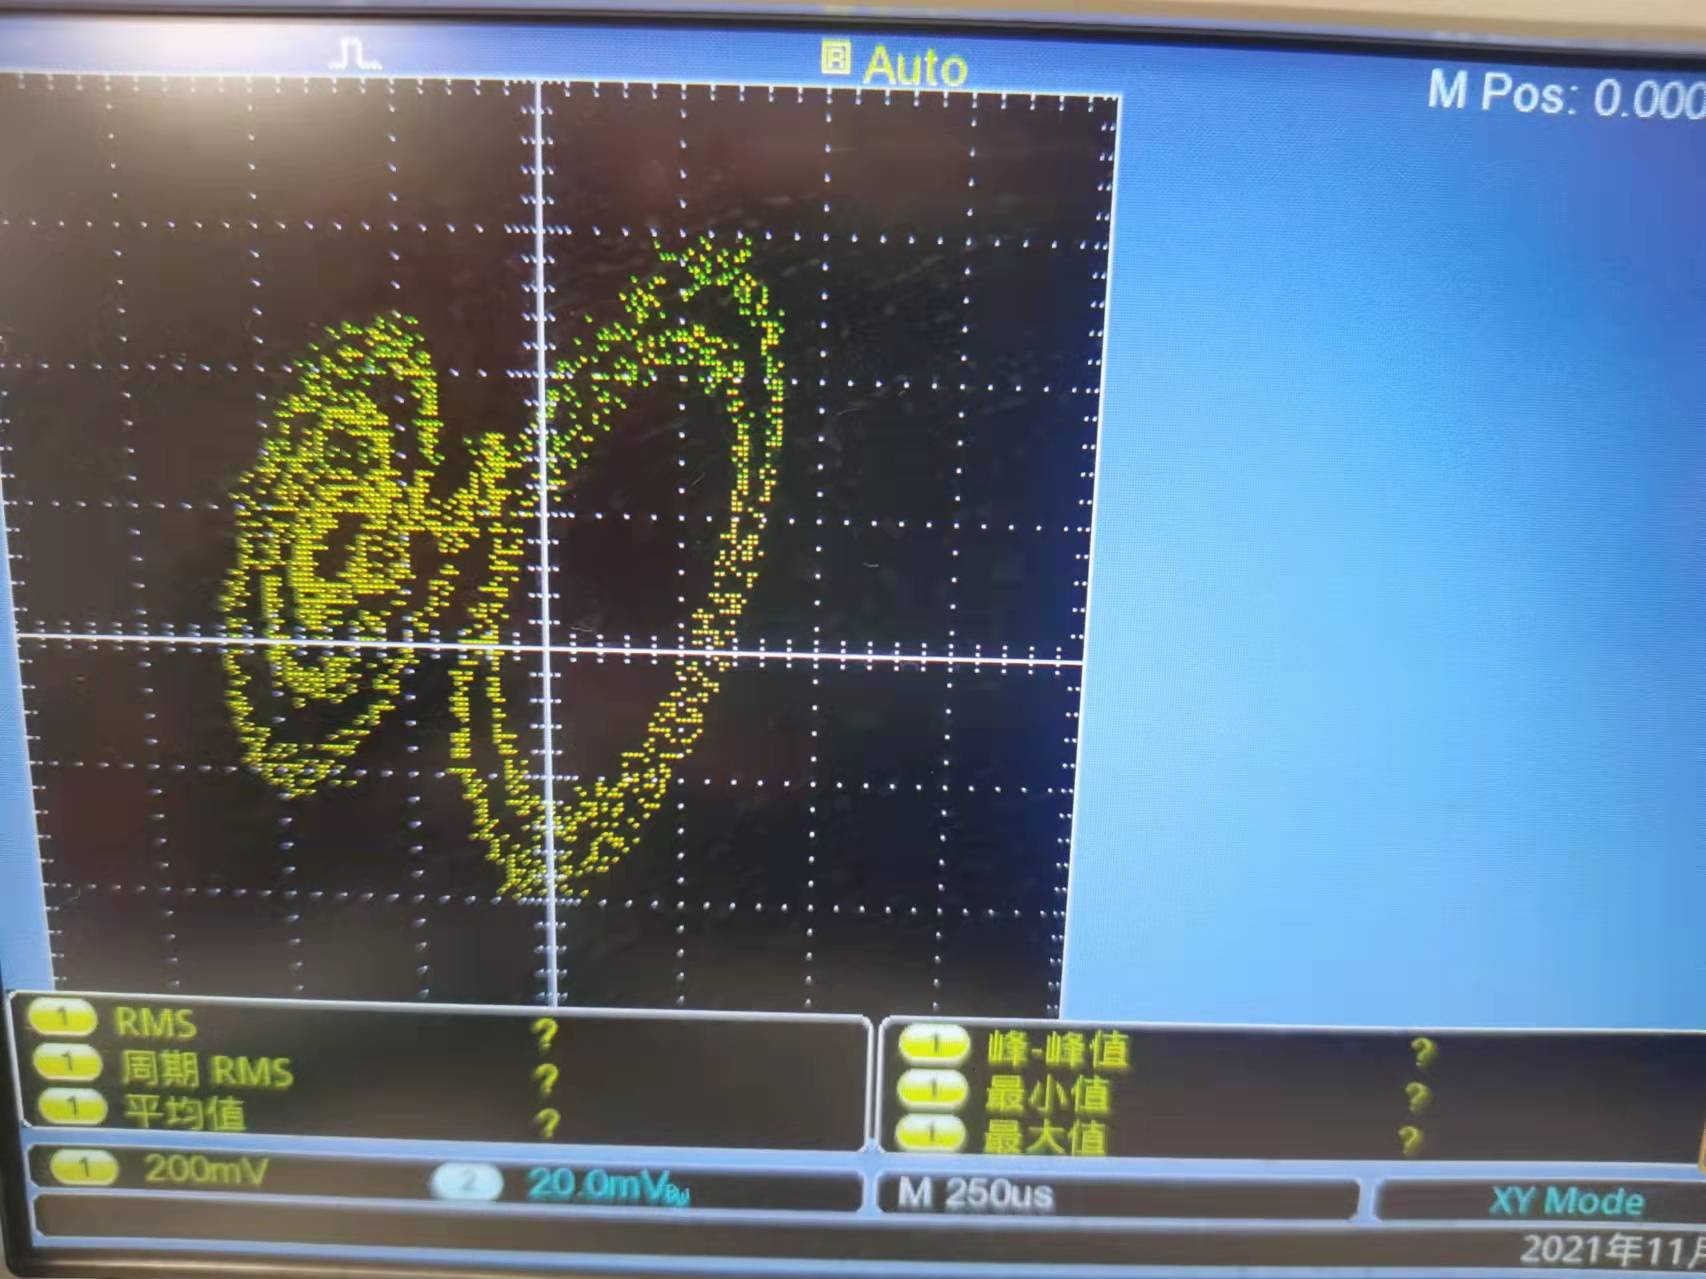
\includegraphics[width=2in]{1-3-30.5k-1-2-r.jpg}
      \caption{$v_{1} - v_{2}$}
      \end{minipage}%
    }%
  \end{figure}

 $R_5 = 31k \Omega$:

\begin{figure}[H]
  \centering
    \subfigure{
    \begin{minipage}[t]{0.33\linewidth}
    \centering
    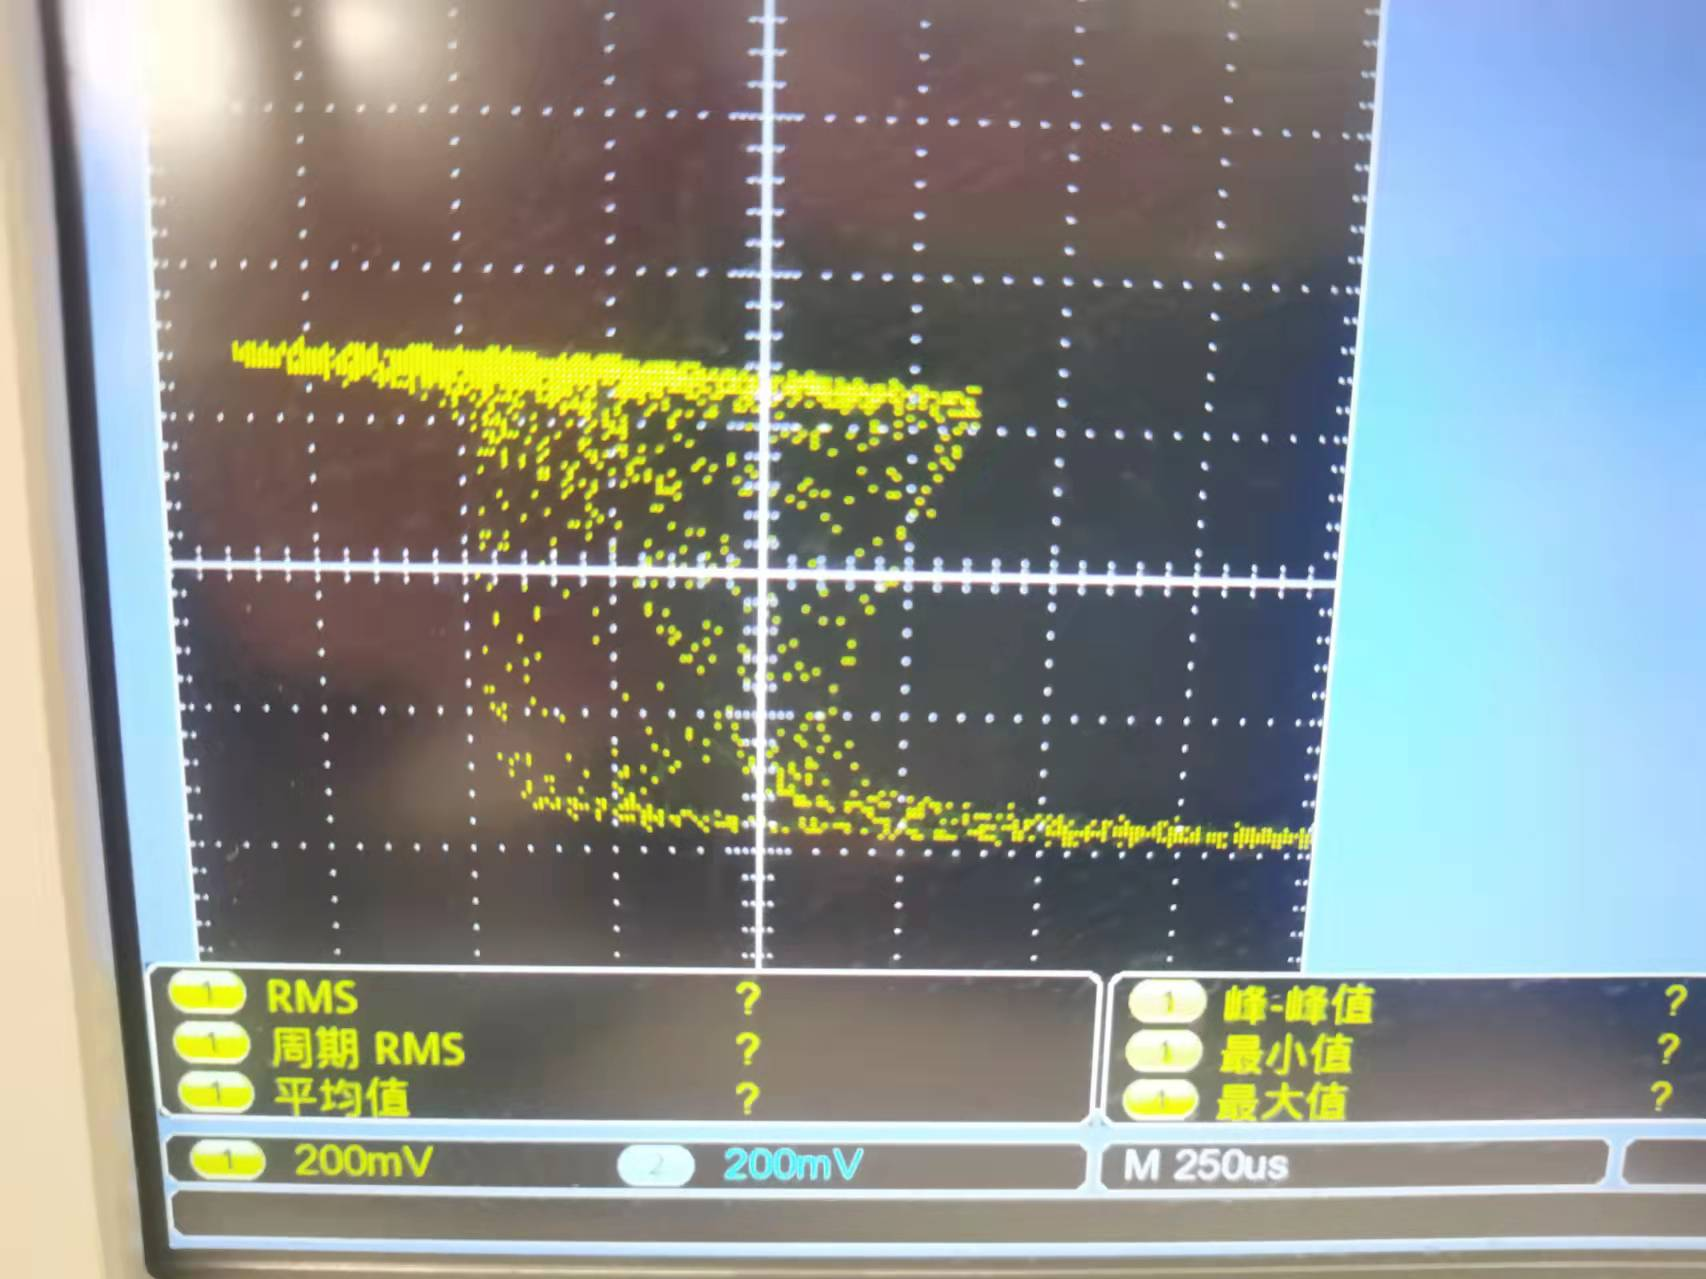
\includegraphics[width=2in]{1-3-31k-ce1ce2-r.jpg}
    \caption{$v_{CE1} - v_{CE2}$}
    \end{minipage}%
  }%
  \subfigure{
    \begin{minipage}[t]{0.33\linewidth}
    \centering
    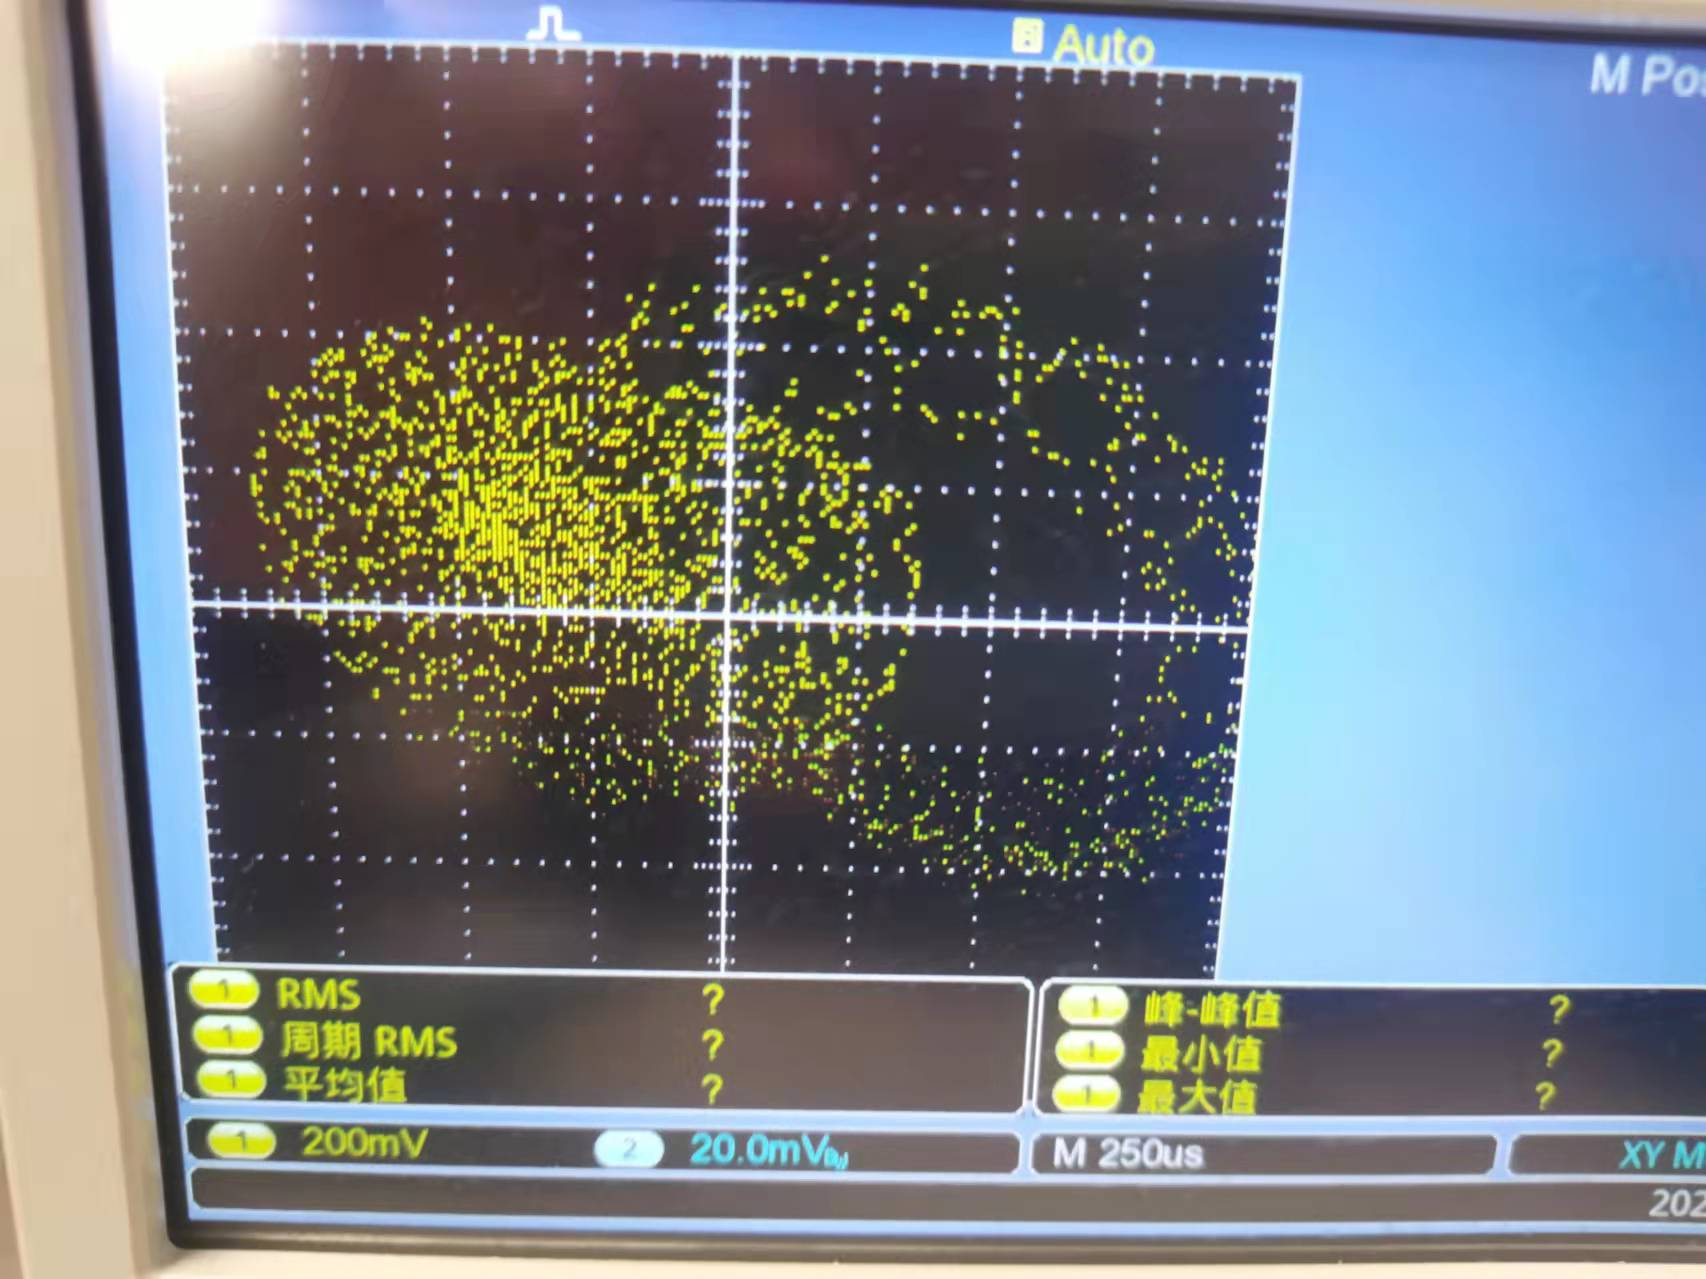
\includegraphics[width=2in]{1-3-31k-ce1-2-r.jpg}
    \caption{$v_{CE1} - v_{2}$}
    \end{minipage}%
  }%
  \subfigure{
    \begin{minipage}[t]{0.33\linewidth}
    \centering
    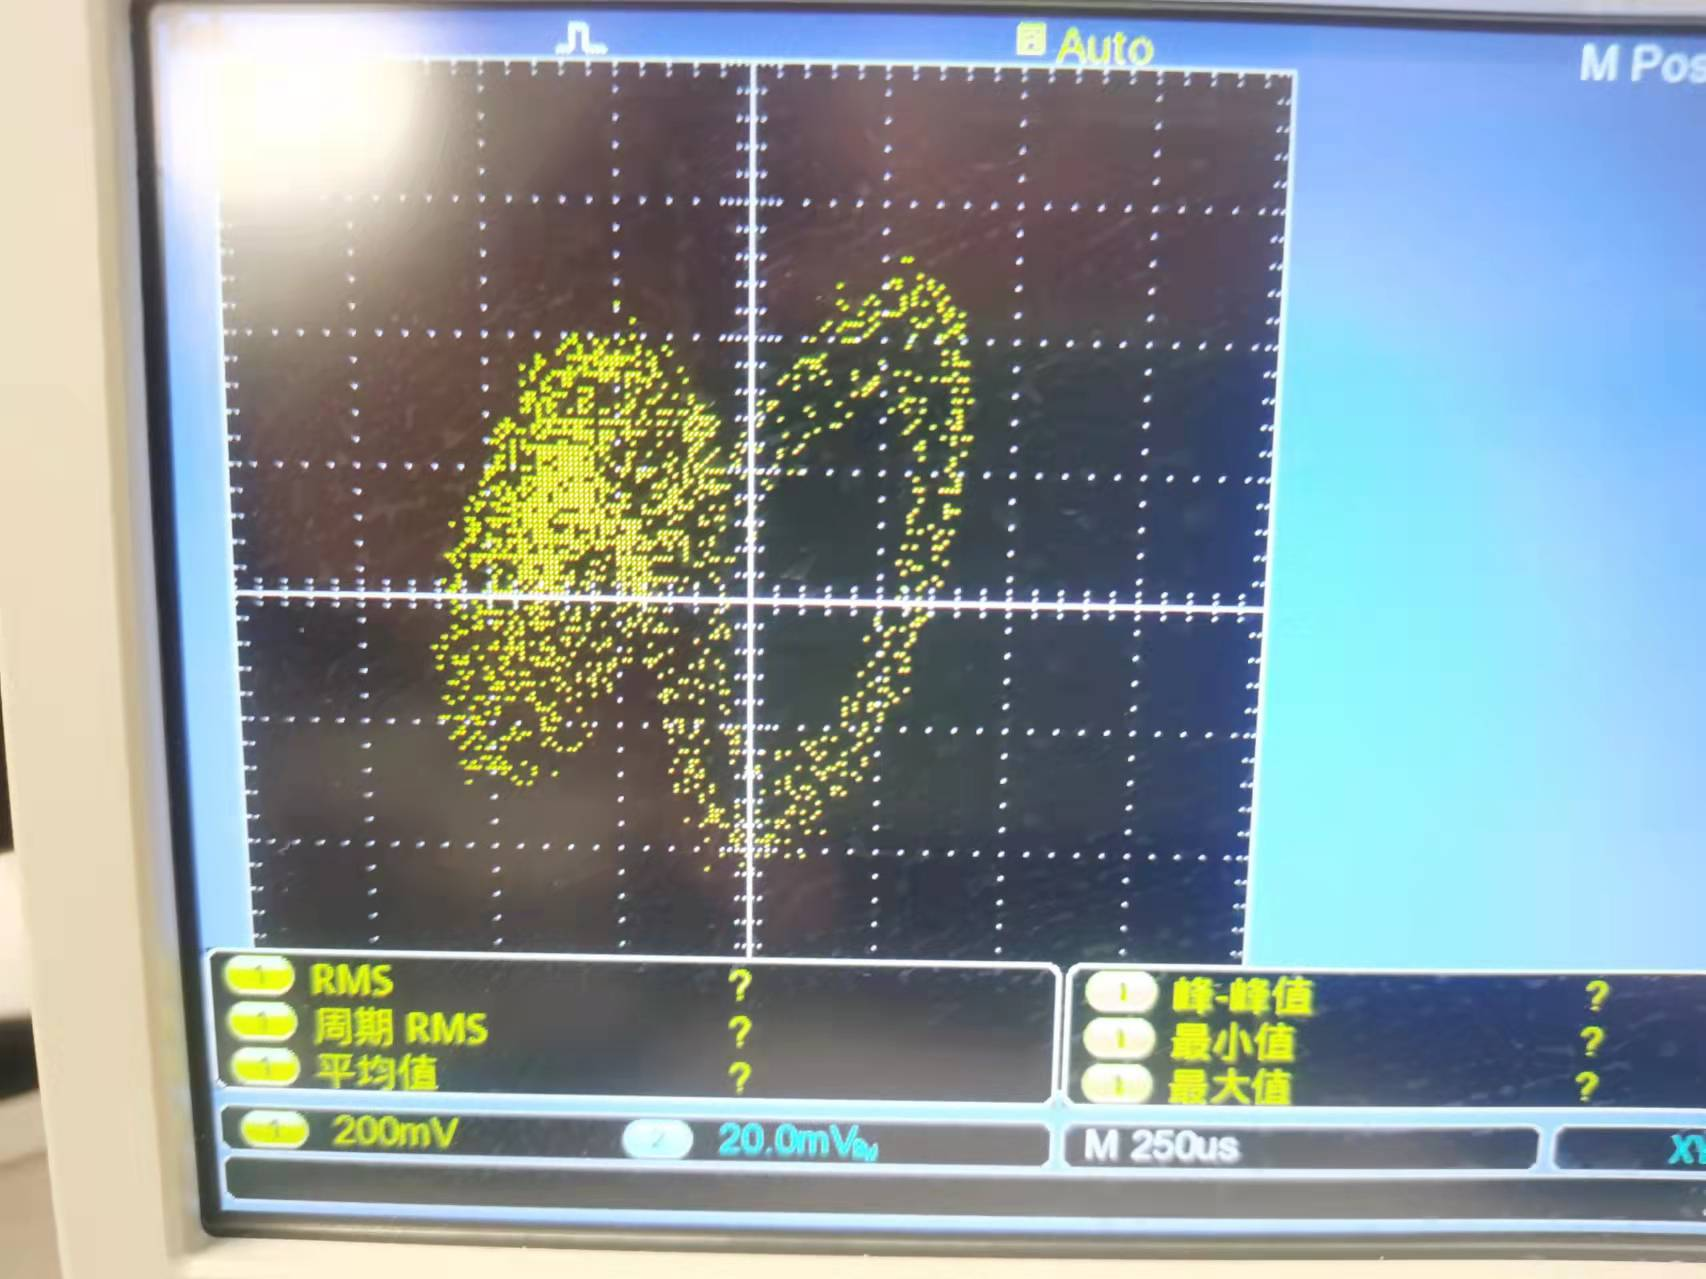
\includegraphics[width=2in]{1-3-31k-1-2-r.jpg}
    \caption{$v_{1} - v_{2}$}
    \end{minipage}%
  }%
\end{figure}
  $R_5 = 31.5k \Omega$:

  \begin{figure}[H]
    \centering
      \subfigure{
      \begin{minipage}[t]{0.33\linewidth}
      \centering
      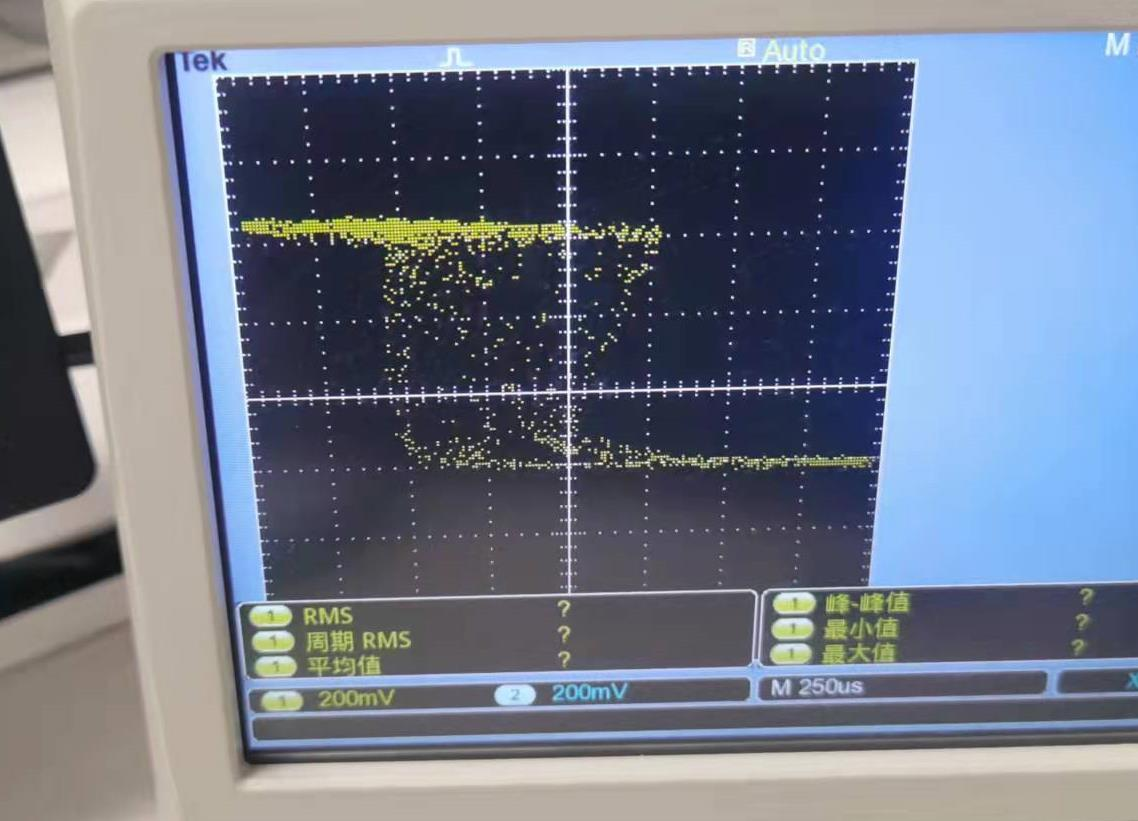
\includegraphics[width=2in]{1-3-31.5k-ce1ce2-r.jpg}
      \caption{$v_{CE1} - v_{CE2}$}
      \end{minipage}%
    }%
    \subfigure{
      \begin{minipage}[t]{0.33\linewidth}
      \centering
      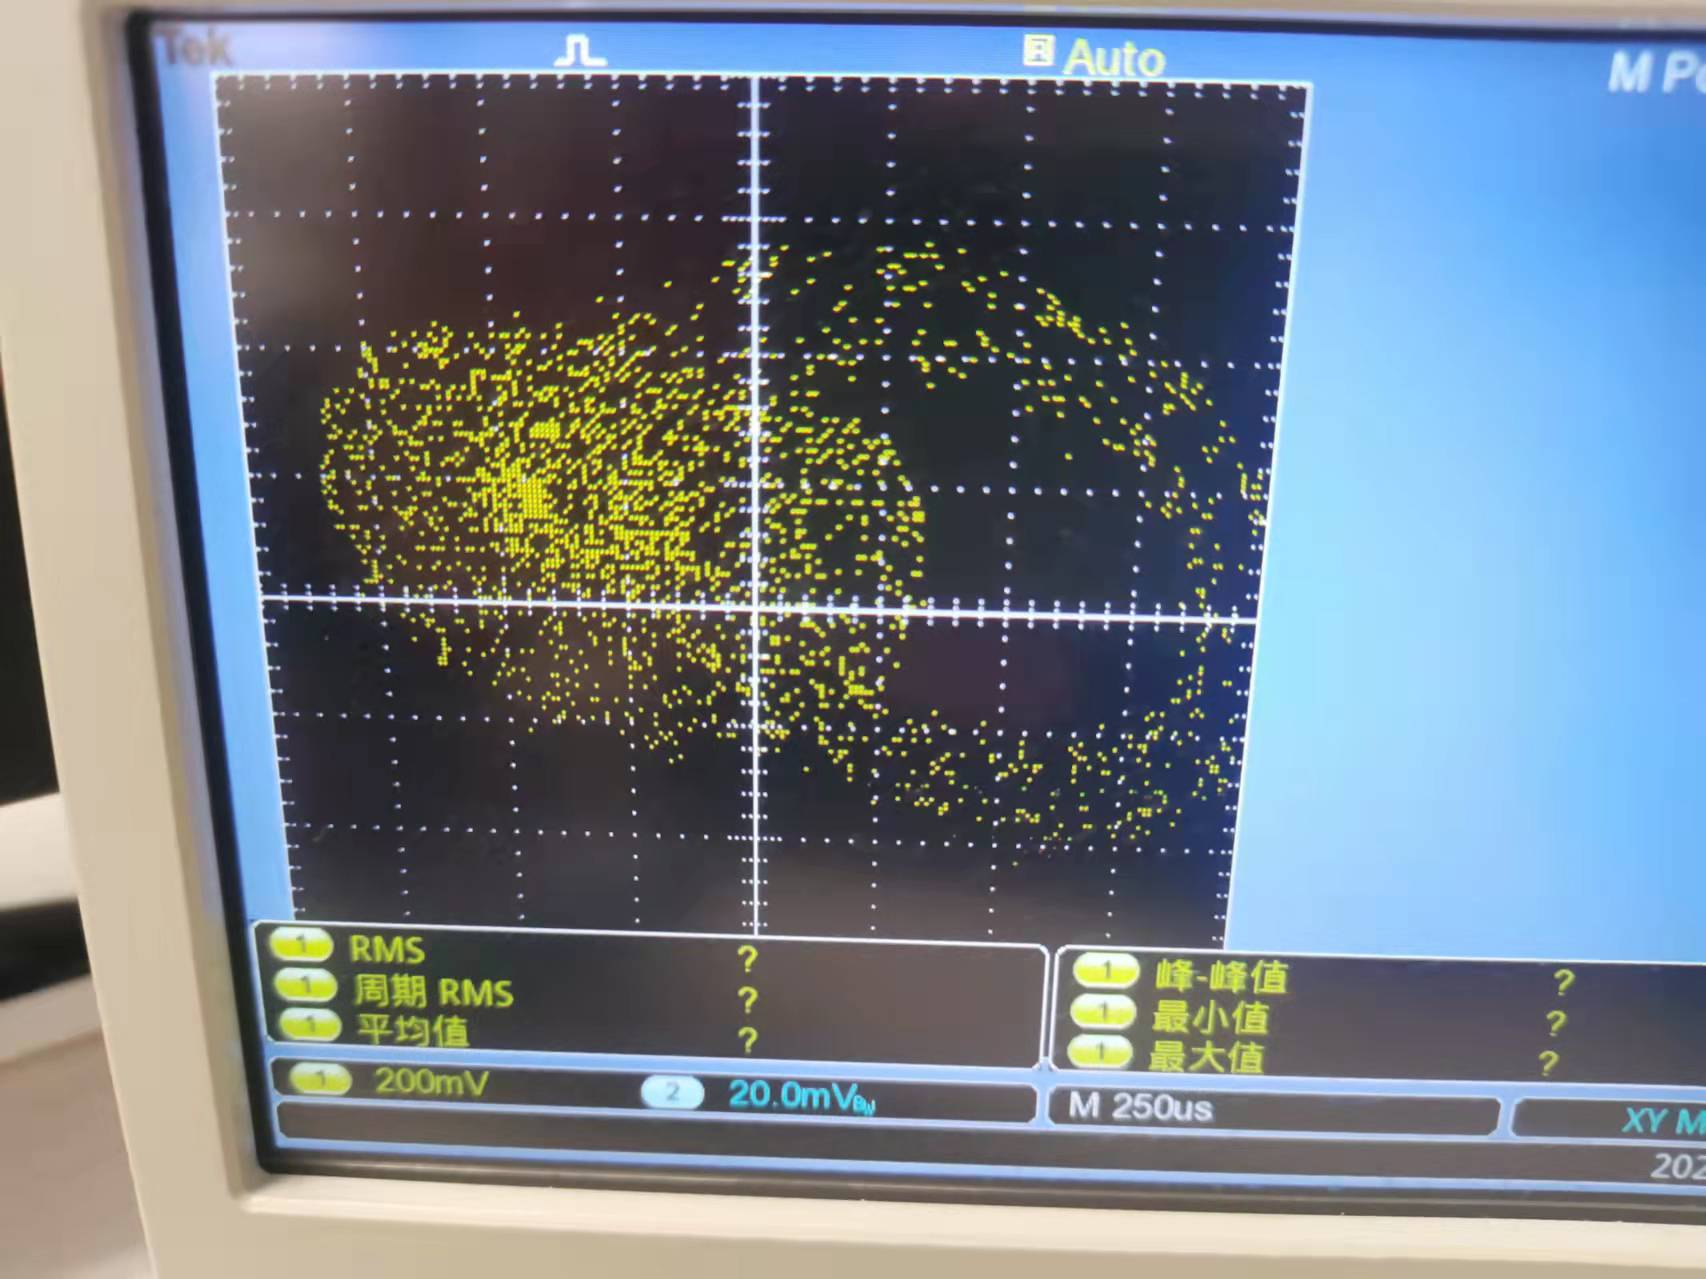
\includegraphics[width=2in]{1-3-31.5k-ce1-2-r.jpg}
      \caption{$v_{CE1} - v_{2}$}
      \end{minipage}%
    }%
    \subfigure{
      \begin{minipage}[t]{0.33\linewidth}
      \centering
      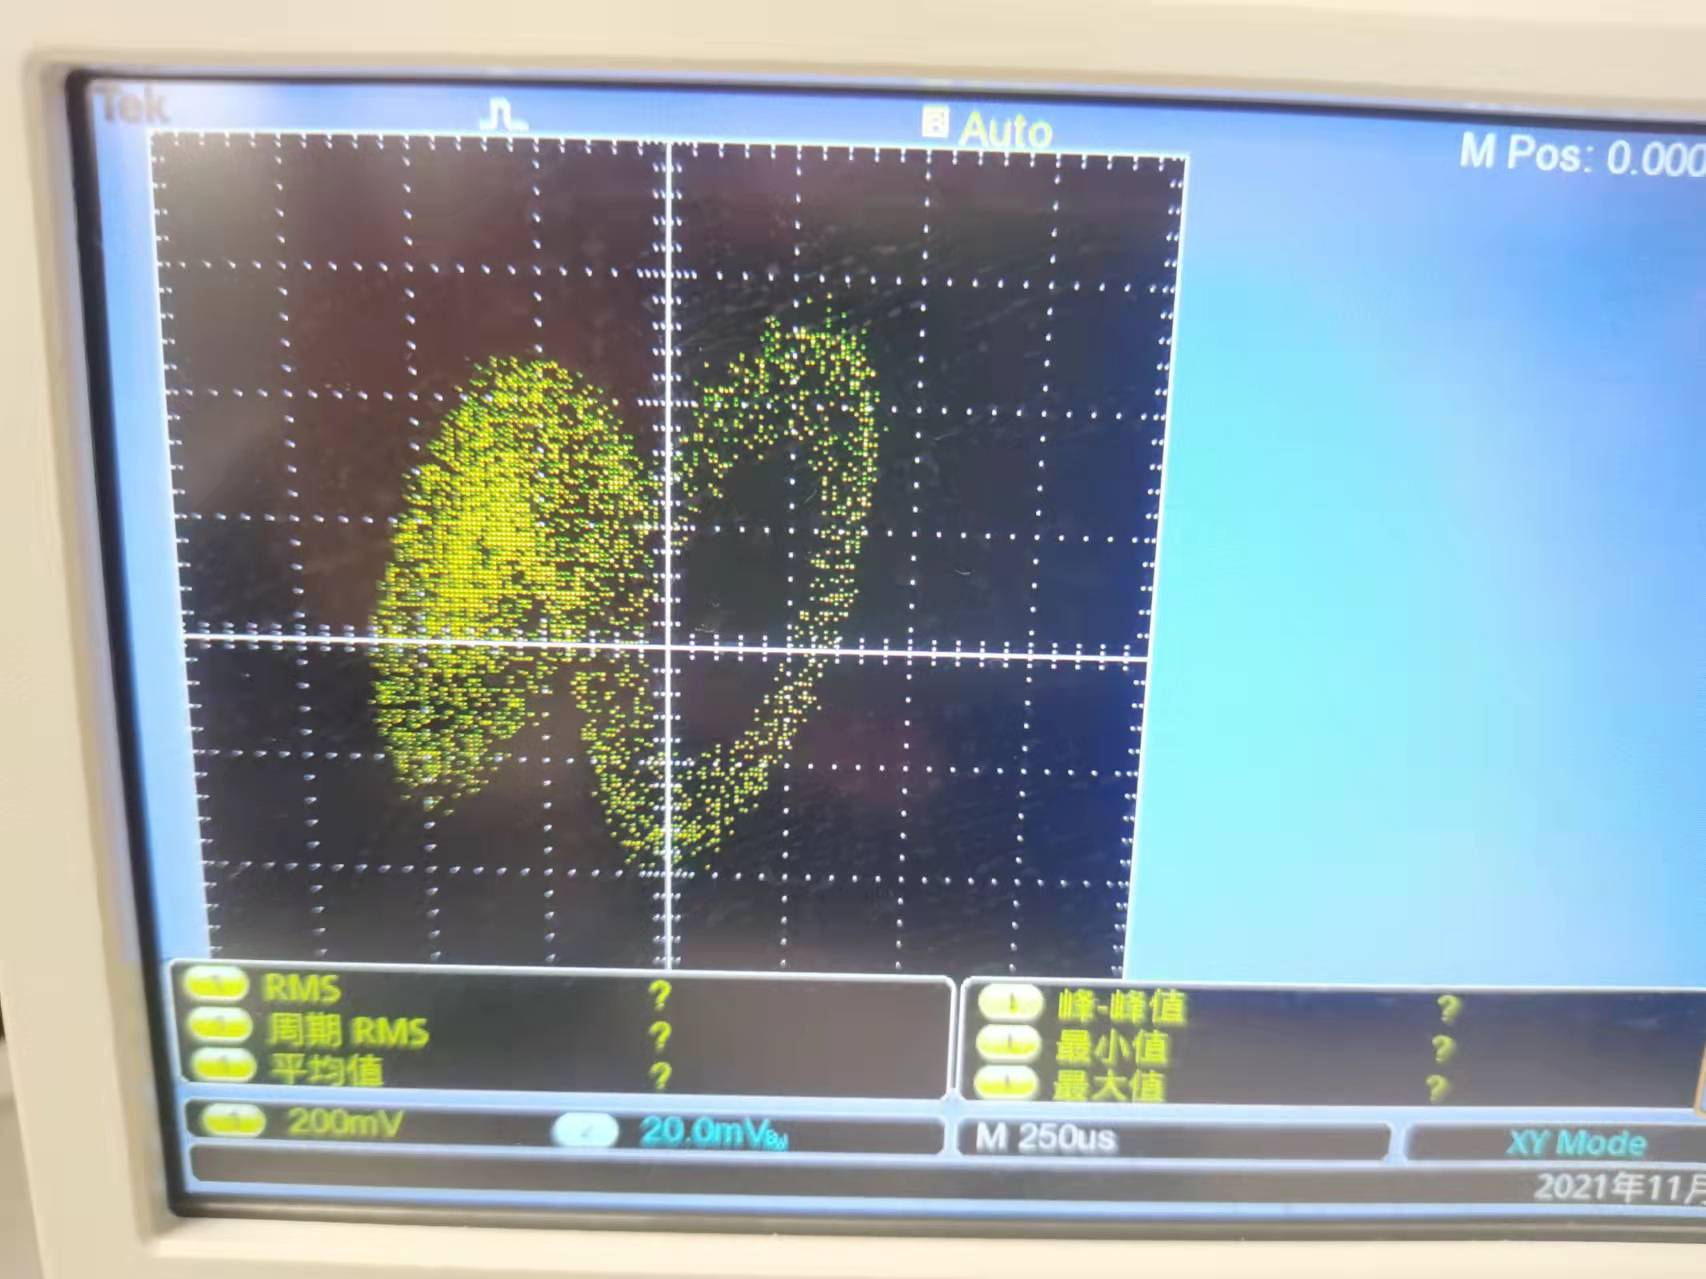
\includegraphics[width=2in]{1-3-31.5k-1-2-r.jpg}
      \caption{$v_{1} - v_{2}$}
      \end{minipage}%
    }%
  \end{figure}
    $R_5 = 32k \Omega$:

    \begin{figure}[H]
      \centering
        \subfigure{
        \begin{minipage}[t]{0.33\linewidth}
        \centering
        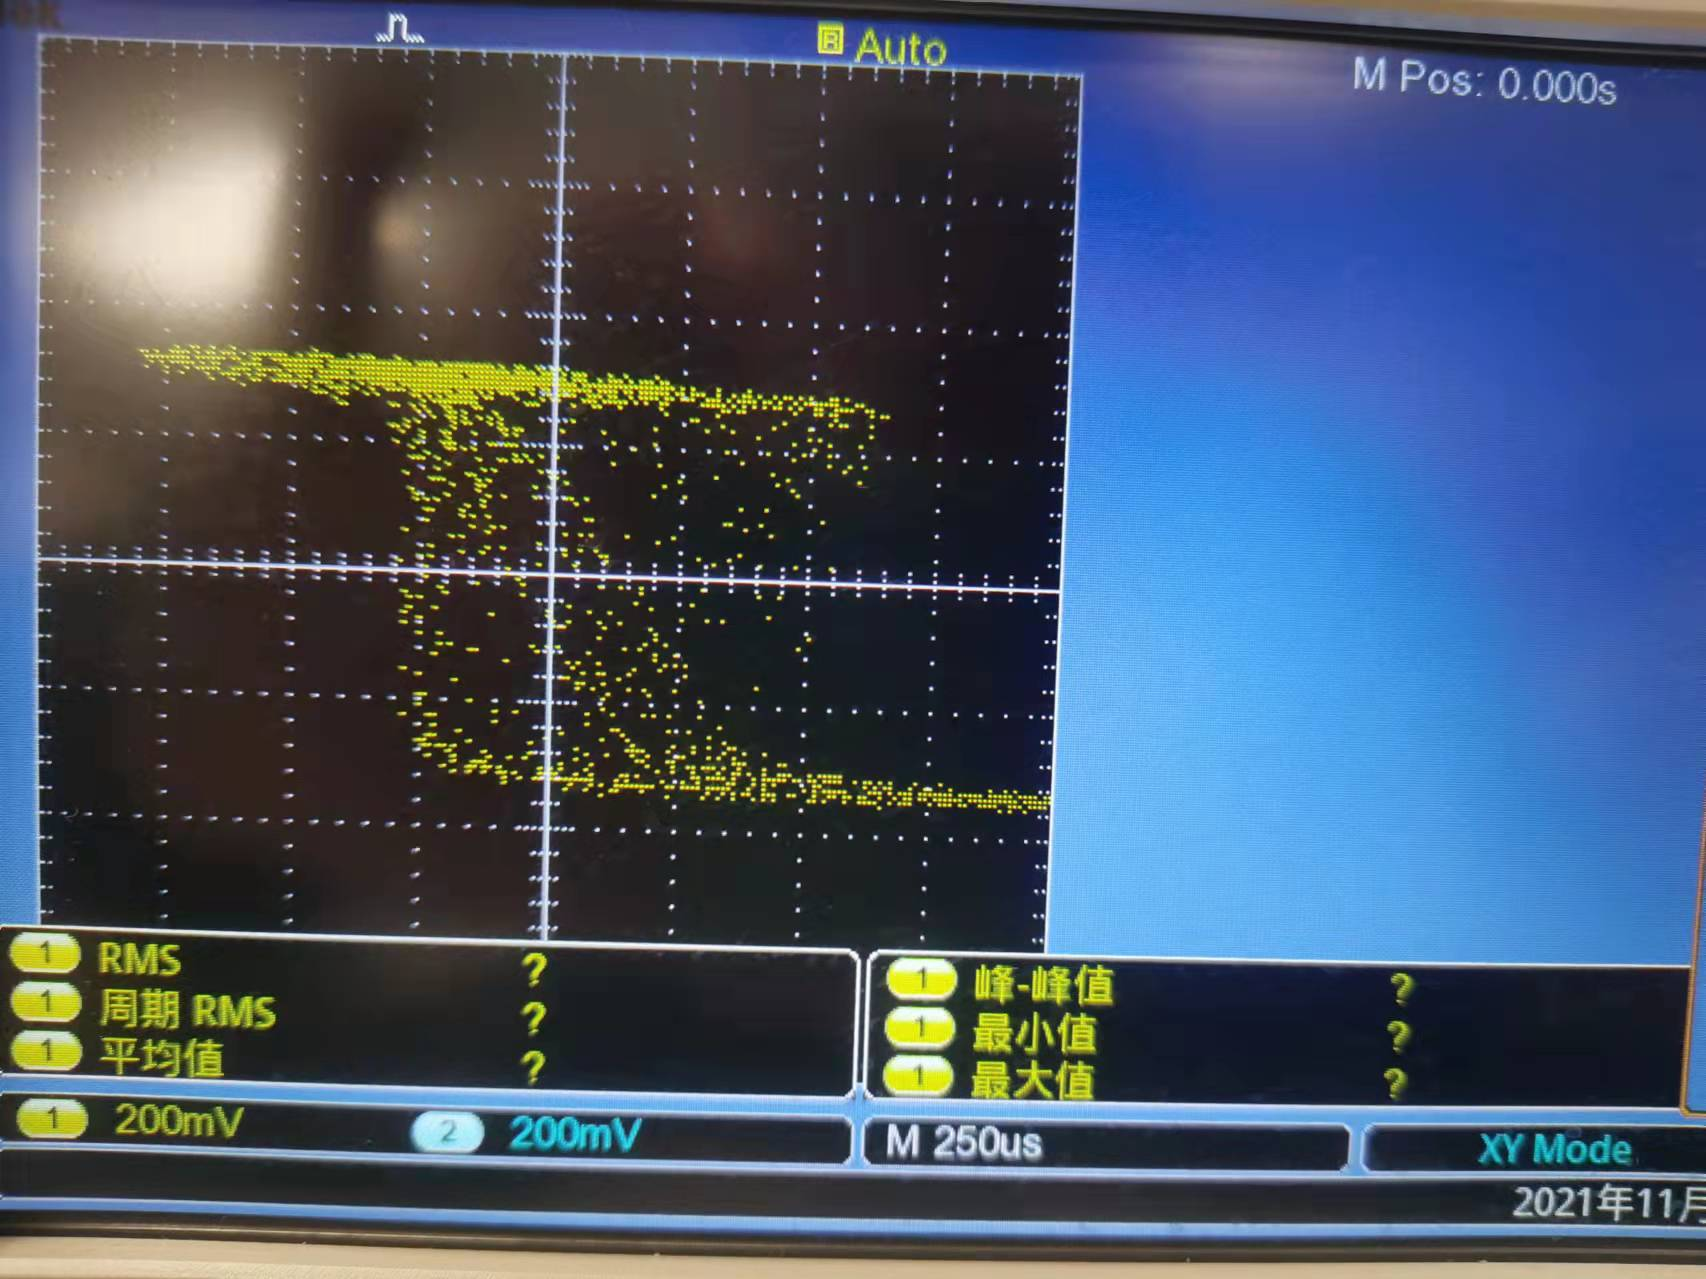
\includegraphics[width=2in]{1-3-32k-ce1ce2-r.jpg}
        \caption{$v_{CE1} - v_{CE2}$}
        \end{minipage}%
      }%
      \subfigure{
        \begin{minipage}[t]{0.33\linewidth}
        \centering
        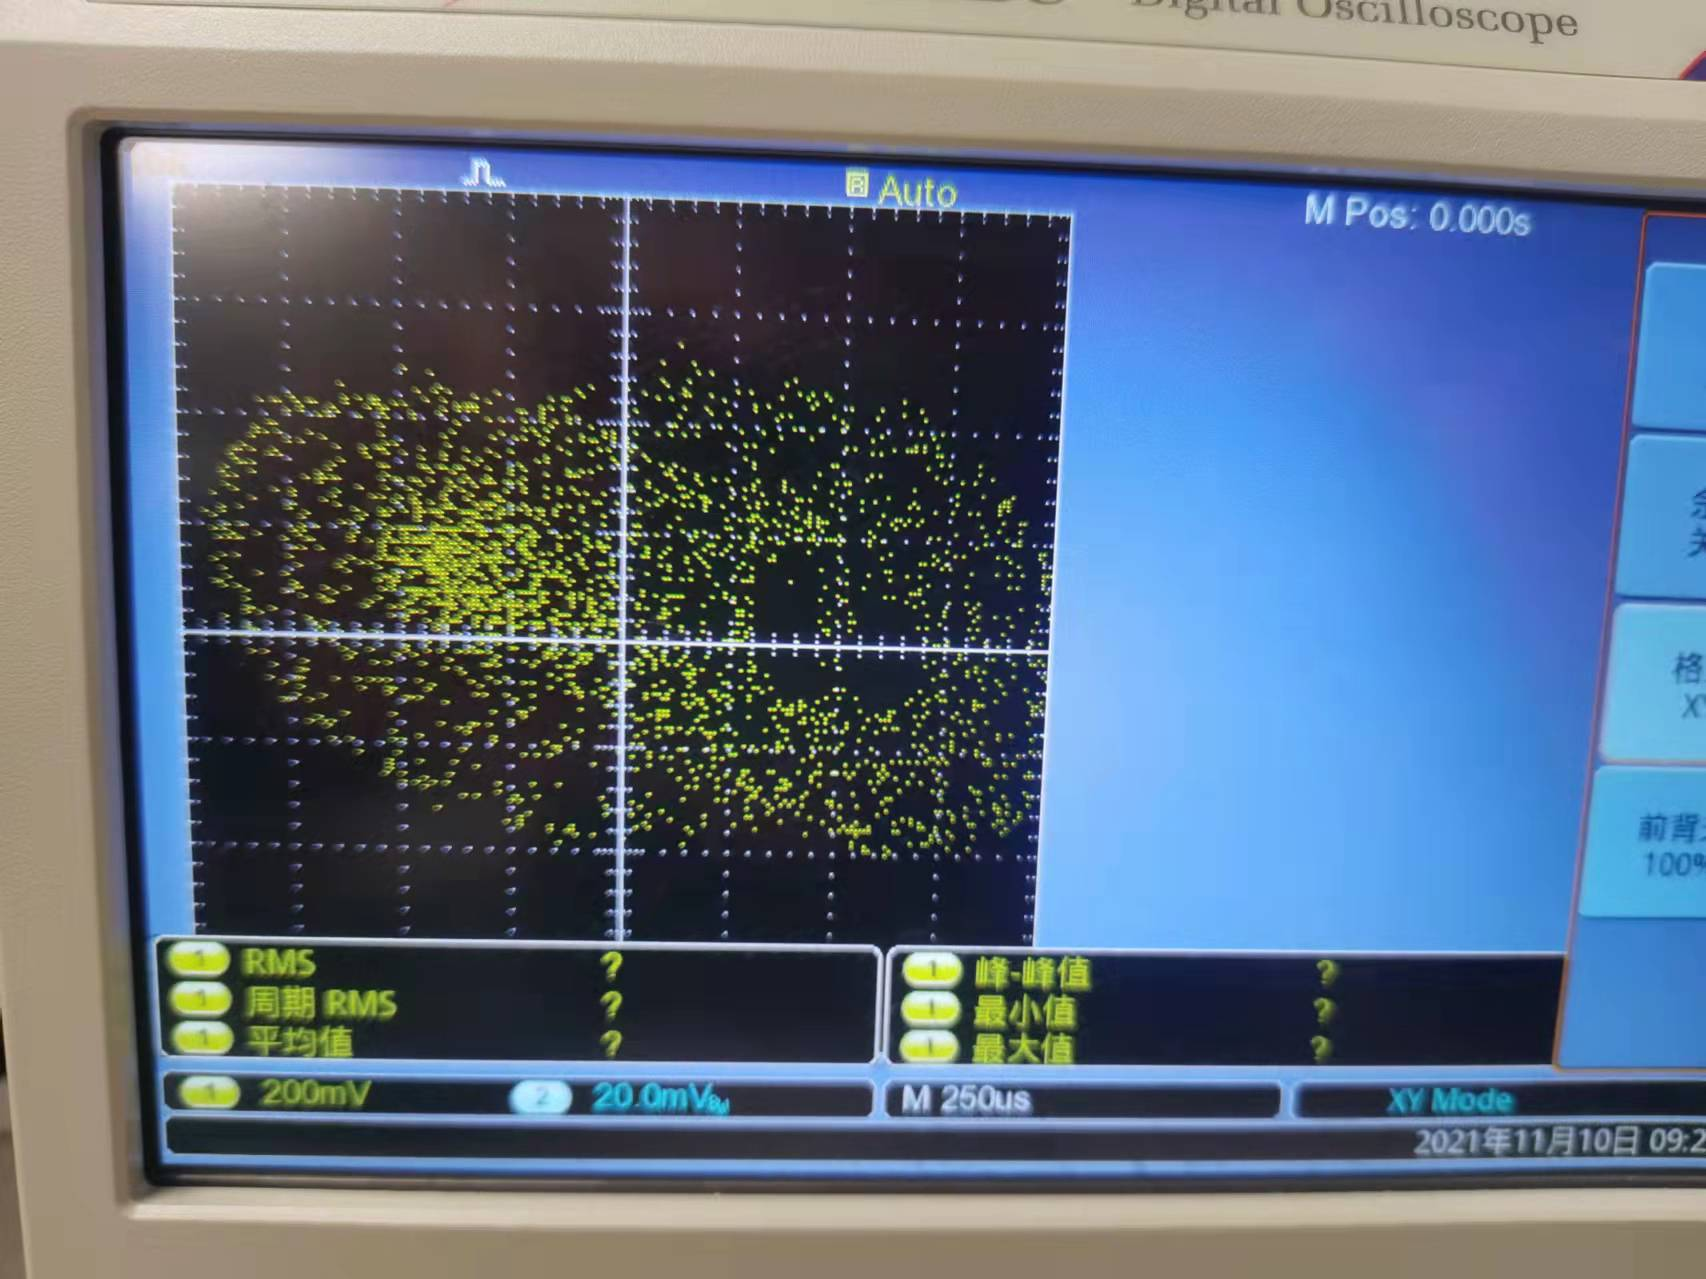
\includegraphics[width=2in]{1-3-32k-ce1-2-r.jpg}
        \caption{$v_{CE1} - v_{2}$}
        \end{minipage}%
      }%
      \subfigure{
        \begin{minipage}[t]{0.33\linewidth}
        \centering
        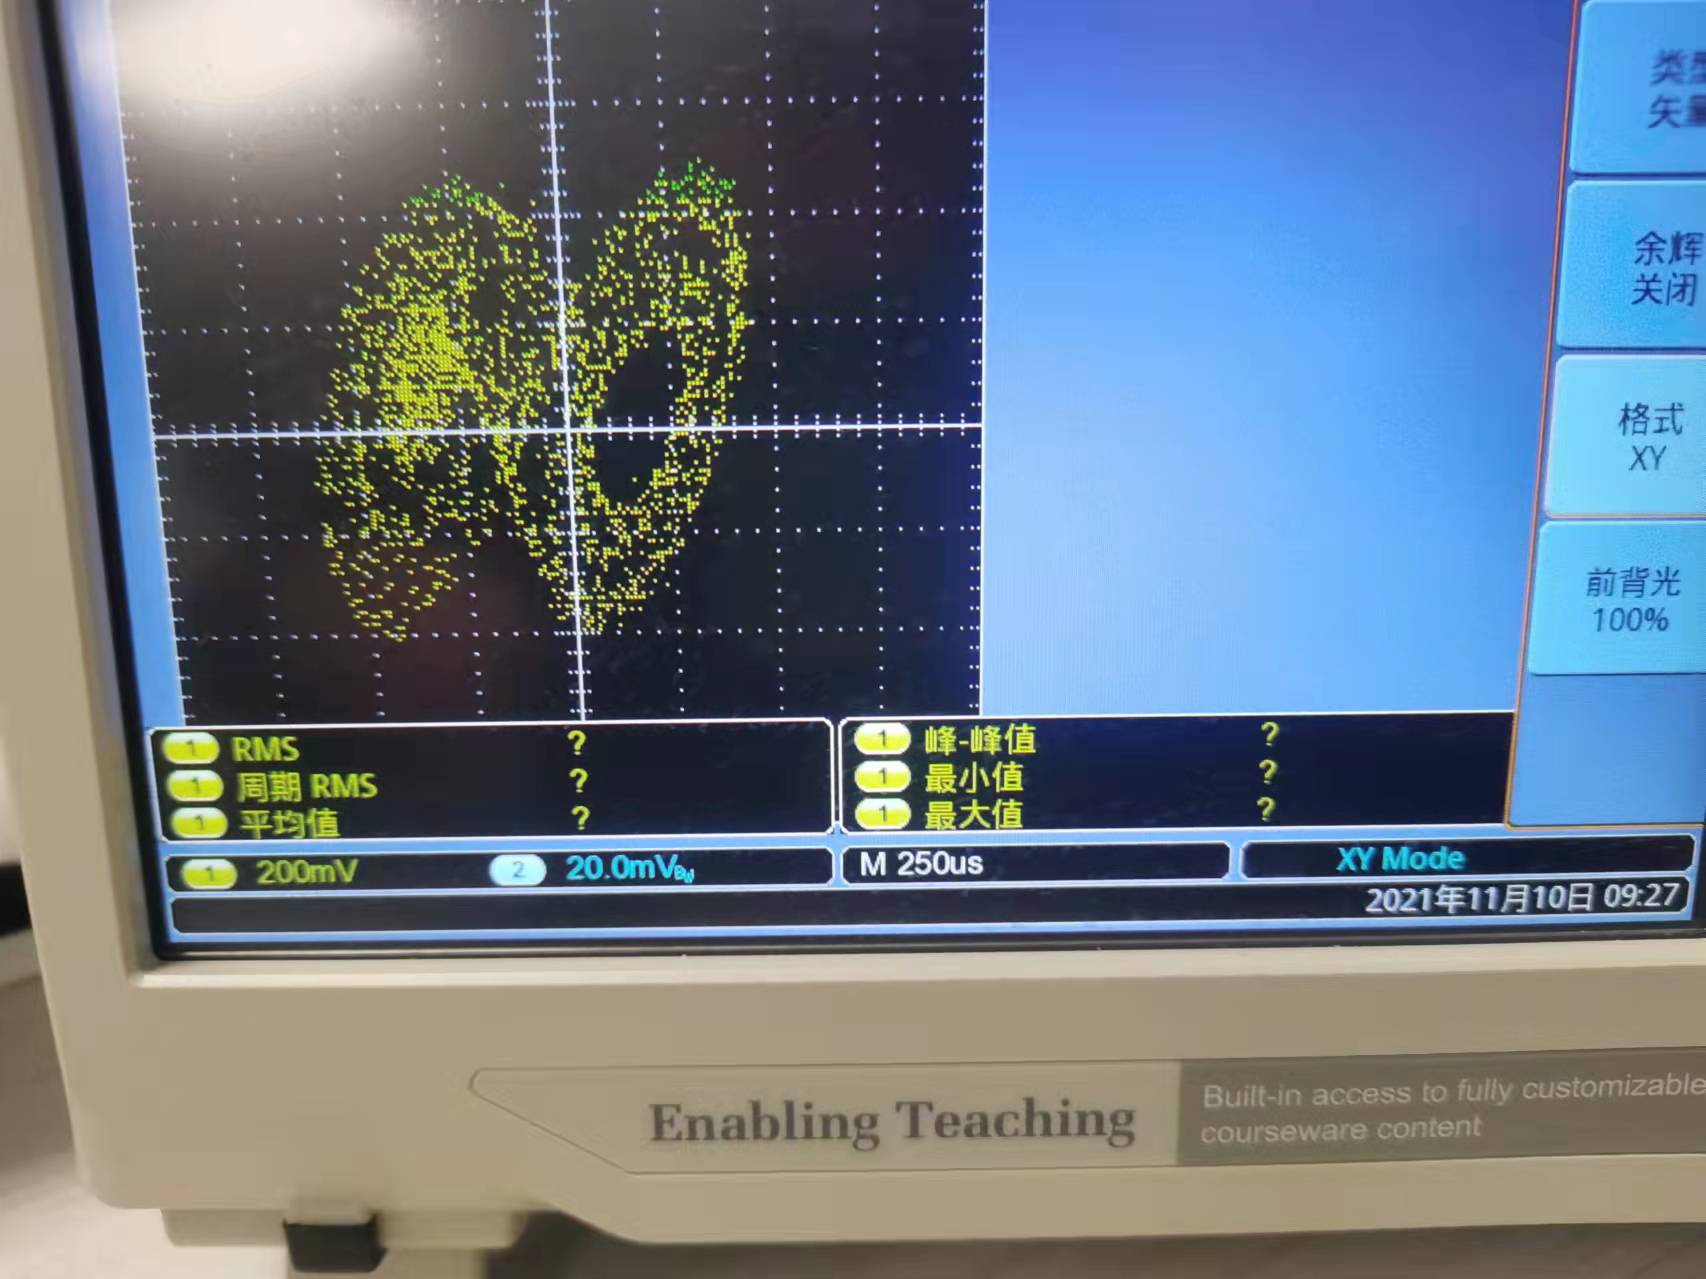
\includegraphics[width=2in]{1-3-32k-1-2-r.jpg}
        \caption{$v_{1} - v_{2}$}
        \end{minipage}%
      }%
  
\end{figure}

波形与仿真结果相近。

\section*{思考}

\subsection*{1.电路输出波形的振荡频率由什么决定?}

电路输出波形的振荡频率由选频电路的幅频特性决定。

\subsection*{2.R2 为什么取 5kΩ 而不是 10kΩ?}

$R_2$取$10k \Omega$的时候,下方电路起到开关作用,导致无法发生混沌。

\subsection*{3.改变 R5 值的作用是什么?}

观察$R_5$变化的情况下电路波形的图像变化,可以找到混沌电路发生条件下$R_5$的大致范围。

\subsection*{4.T2 工作在什么状态?}

$T2$交替工作在线性放大区和截止区。

\subsection*{5.虚线框中电路的作用。}

虚线中的电路起到了开关的作用,当$T2$处于开的状态,即$u_{C2}>0$,
上部振荡电路开始起振。而$T_2$处于关的状态时,即$T_2$截止,上方电路振荡达到稳定。
而上方电路的电压变化会反过来引起下方开关的开闭,两者互相作用,形成混沌系统。

\end{document}